\documentclass[11pt]{article}

\usepackage[margin=1in]{geometry}
\usepackage[T1]{fontenc}
\usepackage{lmodern}
\usepackage{microtype}
\usepackage{amsmath,amssymb,mathtools}
\usepackage{graphicx}
\usepackage[section]{placeins}
\usepackage{booktabs,array}
\usepackage{enumitem}
\usepackage[most]{tcolorbox}
\usepackage[colorlinks=true,linkcolor=blue!50!black,citecolor=blue!50!black,urlcolor=blue!50!black]{hyperref}
\usepackage[capitalise,nameinlink]{cleveref}

\graphicspath{{figures/}}
\setlist{nosep,leftmargin=*}
\numberwithin{equation}{section}

% --- notation -----------------------------------------------------------------
\newcommand{\dd}{\mathrm{d}}
\newcommand{\avg}[1]{\langle #1\rangle}
\newcommand{\given}{\,|\,}
\newcommand{\nodd}{\sum_{n\ \mathrm{odd}}}
% Equation numbers in Gardiner, Handbook of Stochastic Methods, 2nd ed.
\newcommand{\G}[1]{[G~(#1)]}
\newcommand{\Gs}[1]{[G~\S#1]}

% "Setup and key results" box at the top of each example.
\newtcolorbox{keyresults}[1][]{enhanced, colback=black!3, colframe=black!35,
  boxrule=0.4pt, arc=1pt, left=6pt, right=6pt, top=4pt, bottom=4pt,
  colbacktitle=black!10, coltitle=black, fonttitle=\bfseries\small,
  title={Setup and key results}, #1}

\title{Fokker--Planck equation: worked examples}
\author{Sean Ericson}
\renewcommand{\today}{\number\day\space\ifcase\month\or January\or February\or March\or April\or May\or June\or
  July\or August\or September\or October\or November\or December\fi\space\number\year}
\date{Started 26 October 2026 \quad$\cdot$\quad compiled \today}

\begin{document}
\maketitle

\noindent
A running log of exactly solvable one-dimensional Fokker--Planck problems: setup, spectrum,
propagator, long-time behaviour, first-passage quantities and figures. Notation follows Gardiner's
\emph{Handbook of Stochastic Methods}, 2nd ed.~\cite{gardiner}; \G{5.2.100} means equation (5.2.100)
there. The figures are made by \texttt{scripts/make\_figures.py}, which also checks every boxed formula
numerically (\cref{app:checks}). The same examples can be run interactively in \texttt{sde-explorer}.

\begin{table}[h]
\centering
\footnotesize
\renewcommand{\arraystretch}{1.3}
\setlength{\tabcolsep}{4pt}
\begin{tabular}{@{}l l l l l@{}}
\toprule
\S & Domain, walls & $Q_\lambda$ (backward) & $\lambda$ & $t\to\infty$ \\
\midrule
\multicolumn{5}{@{}l}{\emph{Free diffusion, $A=0$, $B=D$}} \\
\ref{sec:line}          & $(-\infty,\infty)$     & $e^{ikx}$, $k\in\mathbb R$ & $Dk^2/2$ & Gaussian, width $\sqrt{Dt}$ \\
\ref{sec:hl-reflecting} & $(0,\infty)$, refl.\ 0 & $\cos kx$, $k\ge0$ & $Dk^2/2$ & half-Gaussian, width $\sqrt{Dt}$ \\
\ref{sec:hl-absorbing}  & $(0,\infty)$, abs.\ 0  & $\sin kx$, $k>0$   & $Dk^2/2$ & $S\sim t^{-1/2}$; no QSD \\
\ref{sec:reflecting} & $(0,L)$, reflecting & $\cos(n\pi x/L)$, $n\ge0$ & $n^2\pi^2D/2L^2$ & $p_s=1/L$ \\
\ref{sec:absorbing}  & $(0,L)$, absorbing  & $\sin(n\pi x/L)$, $n\ge1$ & $n^2\pi^2D/2L^2$ & QSD $\propto\sin(\pi x/L)$ \\
\ref{sec:mixed}      & $(0,L)$, refl.\ 0, abs.\ $L$ & $\cos\frac{(2n+1)\pi x}{2L}$, $n\ge0$ & $(2n+1)^2\pi^2D/8L^2$ & QSD $\propto\cos(\pi x/2L)$ \\
\ref{sec:circle}        & circle $\mathbb R/L\mathbb Z$ & $e^{\pm iq_mx}$, $q_m=2\pi m/L$ & $Dq_m^2/2$, doublets & $p_s=1/L$ \\
\midrule
\multicolumn{5}{@{}l}{\emph{Constant drift, $A=v$, $B=D$; $\alpha=v/D$, $Q_\lambda=e^{-\alpha x}u_n$}} \\
\ref{sec:drift-line}          & $(-\infty,\infty)$     & $u=e^{ikx}$ & $\frac{v^2}{2D}+\frac{Dk^2}{2}$ & $g(x-x_0-vt)$ \\
\ref{sec:drift-hl-reflecting} & $(0,\infty)$, refl.\ 0 & $u=\cos kx+\frac\alpha k\sin kx$ & $\{0\}\cup[\frac{v^2}{2D},\infty)$ if $v<0$ & $p_s\propto e^{-2|v|x/D}$ if $v<0$ \\
\ref{sec:drift-hl-absorbing}  & $(0,\infty)$, abs.\ 0  & $u=\sin kx$ & $\frac{v^2}{2D}+\frac{Dk^2}{2}$ & $v<0$: QSD continuum \\
\ref{sec:drift-reflecting} & $(0,L)$, reflecting & $u_n=\cos k_nx+\frac{\alpha}{k_n}\sin k_nx$ & $\frac{v^2}{2D}+\frac{n^2\pi^2D}{2L^2}$, and $0$ & $p_s\propto e^{2vx/D}$ \\
\ref{sec:drift-absorbing} & $(0,L)$, absorbing & $u_n=\sin k_nx$ & $\frac{v^2}{2D}+\frac{n^2\pi^2D}{2L^2}$ & QSD $\propto e^{\alpha x}\sin k_1x$ \\
\ref{sec:drift-mixed} & $(0,L)$, refl.\ 0, abs.\ $L$ & $\cos k_nx+\frac{\alpha}{k_n}\sin k_nx$ & $\frac{v^2}{2D}+\frac{Dk_n^2}{2}$, $\tan k_nL=-\frac{k_n}{\alpha}$ & QSD; Arrhenius \\
\ref{sec:drift-circle}        & circle                 & $e^{iq_mx}$, $m\in\mathbb Z$ (no gauge) & $\frac{Dq_m^2}{2}+ivq_m$ & $p_s=1/L$, $J_s=v/L$ \\
\midrule
\multicolumn{5}{@{}l}{\emph{Ornstein--Uhlenbeck, $A=-kx$, $B=D$; $\ell=\sqrt{D/k}$, $\xi=x/\ell$, walls measured from the bottom}} \\
\ref{sec:ou-line}          & $(-\infty,\infty)$     & $H_n(\xi)$ & $nk$ & $p_s\propto e^{-\xi^2}$, gap $k$ \\
\ref{sec:ou-hl-reflecting} & $(0,\infty)$, refl.\ 0 & even $H_n$ & $2mk$ & half-Gaussian, gap $2k$ \\
\ref{sec:ou-hl-absorbing}  & $(0,\infty)$, abs.\ 0  & odd $H_n$  & $(2m+1)k$ & QSDs $\lambda\in(0,k]$; Rayleigh \\
\ref{sec:ou-reflecting}    & $(0,L)$, reflecting    & $M(-\frac\nu2,\frac12,\xi^2)$ & $\nu_nk$ & truncated half-Gaussian \\
\ref{sec:ou-absorbing}     & $(0,L)$, absorbing     & $\xi M(\frac{1-\nu}2,\frac32,\xi^2)$ & $\nu_nk$ & QSD: sine $\to$ Rayleigh \\
\ref{sec:ou-mixed}         & $(0,L)$, refl.\ 0, abs.\ $L$ & $M(-\frac\nu2,\frac12,\xi^2)$ & $\nu_nk$ & Kramers escape \\
\ref{sec:ou-circle}        & circle, sawtooth $A$   & sectors of \S\ref{sec:ou-reflecting}, \S\ref{sec:ou-absorbing} & $\nu^{\rm A}_nk$, $(\nu^{\rm A}_n+1)k$ & cusp; Lifson--Jackson \\
\ref{sec:cos-circle}       & circle, $U\propto-\cos\frac xR$ & Fourier recurrence & doublets, $\frac{m^2k}\kappa\to nk$ & von Mises; tilt: NESS \\
\midrule
\multicolumn{5}{@{}l}{\emph{More solvable potentials, $A=-U'$, $B=D$ (\cref{tab:solvable}); arbitrary potentials}} \\
\ref{sec:radial}       & $x>0$, $\frac12kx^2-c\ln x$ & Laguerre $L_n^{(d/2-1)}$ & $2nk$ & chi; $d=2$ Rayleigh \\
\ref{sec:lncosh}       & line, $a\ln\cosh\frac xw$ & Jacobi & $\frac{D}{2w^2}n(2s-n)$, $n<s$ & $\operatorname{sech}^{2s}$; continuum \\
\ref{sec:lncos}        & $|x|<\frac{\pi w}2$, $-a\ln\cos\frac xw$ & Gegenbauer & $nk+\frac{n^2\pi^2D}{2L^2}$ & $\cos^{2s}$ \\
\ref{sec:double-well}  & line, double well & numerical & $\lambda_1\simeq$ Kramers & bimodal; two-state \\
\midrule
\multicolumn{5}{@{}l}{\emph{Interfaces and singular boundaries}} \\
\ref{sec:interface} & line, $B$ jumps at $0$ & $\cos$ on each side & $\frac12D_\pm k^2$ & box: $p_s^+/p_s^-=K$ \\
\ref{sec:sqrt}      & $y>0$, $B=4Dy$ & Laguerre & $2nk$; $(2n+2-d)k$ & gamma; exit if $d\le0$ \\
\ref{sec:qif}       & line, $A=x^2+I$ & $Q_0=1$ only & --- & current through $\infty$ \\
\bottomrule
\end{tabular}
\caption{The examples in these notes, in section order. The third column gives Gardiner's backward eigenfunctions
$Q_\lambda$, up to normalisation; the forward ones are $P_\lambda=p_sQ_\lambda$, except on the circle with a current
and through infinity. Each section's box gives both, normalised (\cref{sec:eigen}).}
\label{tab:overview}
\end{table}

\tableofcontents

% ==============================================================================
\section{Conventions and toolkit}
\label{sec:conventions}

\subsection{Equation, current, boundary conditions}

The forward equation and probability current are
\begin{equation}
  \partial_t p(x,t) = -\partial_x\bigl[A(x)\,p\bigr] + \tfrac12\,\partial_x^2\bigl[B(x)\,p\bigr]
  = -\partial_x J,
  \qquad
  J(x,t) = A\,p - \tfrac12\,\partial_x(B\,p),
  \label{eq:fpe}
\end{equation}
corresponding to the It\^o SDE $\dd x = A\,\dd t + \sqrt{B}\,\dd W$ \G{5.2.1}, \G{5.2.8}. At a wall
$x=a$ \Gs{5.2.1}:
\begin{itemize}
  \item \textbf{reflecting:} $J(a,t)=0$ \G{5.2.13} (for $A=0$, $B$ constant: $\partial_x p=0$);
  \item \textbf{absorbing:} $p(a,t)=0$ \G{5.2.14};
  \item \textbf{at infinity:} $J(\pm\infty,t)=0$ \G{5.2.32}, or $J(+\infty,t)=J(-\infty,t)$ \G{5.2.33} when what
        leaves at one end comes back at the other (\cref{sec:qif});
  \item \textbf{periodic:} not a boundary condition in these notes. The domain is a circle, which has no
        boundary (\cref{sec:circle-toolkit});
  \item \textbf{at an interface} where $A$ or $B$ jumps: $J$ continuous, and $p$ continuous \G{5.2.15}--\G{5.2.16}.
        For a jump in $B$ the second depends on where the noise comes from (\cref{sec:interface});
  \item \textbf{where $B$ vanishes or $A$ diverges} the equation may decide by itself whether any condition is
        allowed: Feller's classification \Gs{5.2.1e} (\cref{sec:sqrt,sec:feller}).
\end{itemize}
The backward equation, in the initial point, is \G{5.2.143}
\begin{equation}
  \partial_t p(x',t\given x,0) = A(x)\,\partial_x p + \tfrac12 B(x)\,\partial_x^2 p .
  \label{eq:backward}
\end{equation}
On the backward side the walls become $p=0$ (absorbing, \G{5.2.67}) and $\partial_xp=0$ (reflecting,
\G{5.2.69}) in the initial point.

\paragraph{Factor of two.} With $A=0$, $B=D$ the equation is $\partial_t p=\tfrac12D\,\partial_x^2p$, so free
motion has $\avg{(\Delta x)^2}=Dt$. Many references (and \texttt{qsd-context.md}) write
$\partial_tp=D'\partial_x^2p$; then $D'=D/2$, and every rate below has $D/2\to D'$. In
\texttt{sde-explorer}, $D=\sigma^2$ where $\sigma$ is the noise amplitude $b$.

\paragraph{Units.} For an interval of length $L$ the natural time is $L^2/D$. The figures use $L=D=1$, so
axes read $x/L$ and $Dt/L^2$. Parts~II and~III use the scales set by the drift instead
(\cref{eq:drift-scales,eq:ou-scales}).

\subsection{Where the equation comes from: overdamped Brownian motion}
\label{sec:physical}

\paragraph{The physical model.} A Brownian particle of mass $m$ in a potential $\mathcal U(x)$, with friction coefficient
$\gamma$ and a heat bath at temperature $T$, obeys Langevin's equations
\begin{equation}
  \dd x=v\,\dd t,\qquad m\,\dd v=-\gamma v\,\dd t-\mathcal U'(x)\,\dd t+\sqrt{2\gamma k_BT}\,\dd W
  \label{eq:langevin}
\end{equation}
\G{5.3.90}--\G{5.3.91}; Gardiner's $\beta$ is our $\gamma$. The strength of the noise is fixed by the
fluctuation--dissipation relation: it is the value for which the Maxwell--Boltzmann density
$\propto e^{-(mv^2/2+\mathcal U)/k_BT}$ is stationary. The Fokker--Planck equation for $p(x,v,t)$ is Kramers' equation
\G{5.3.92}, \G{5.3.97}, in two variables. The one-variable equation of these notes is its high-friction limit.

\paragraph{Eliminating the velocity \Gs{6.4}.} The velocity forgets its past in the time $m/\gamma$ \G{6.4.4}. If
that is shorter than every time on which the position changes, $v$ is slaved to $x$. Setting $m\,\dd v\approx0$
gives $\gamma\,\dd x=-\mathcal U'\,\dd t+\sqrt{2\gamma k_BT}\,\dd W$ \G{6.4.16}--\G{6.4.17}, whose Fokker--Planck
equation is Smoluchowski's \G{6.4.18}. That is \cref{eq:fpe} with
\begin{equation}
  A=-\frac{\mathcal U'}{\gamma},\qquad B=D=\frac{2k_BT}{\gamma},\qquad\text{so}\qquad U=\frac{\mathcal U}{\gamma}
  \quad\text{and}\quad e^{-2U/D}=e^{-\mathcal U/k_BT}.
  \label{eq:dictionary}
\end{equation}
\begin{itemize}
  \item The potential $U$ of these notes is the physical potential divided by the friction. $D/2=k_BT/\gamma$ is
        Einstein's diffusion coefficient: that is the factor of two above. When the notes say that $D/2$ plays the
        role of $k_BT$, they mean $k_BT/\gamma$, in units where $\gamma=1$. The stationary density is the
        Boltzmann factor.
  \item The examples translate as follows:
        \begin{itemize}
          \item Part~II is a constant force $F$, for instance gravity minus buoyancy in Smoluchowski's
                sedimentation problem (\cref{sec:drift-hl-reflecting}): $v=F/\gamma$, and the barometric profile
                $e^{-2x/\ell}$ is $e^{-|F|x/k_BT}$.
          \item Part~III is a harmonic trap of stiffness $\mathcal K$, such as an optical tweezer:
                $k=\mathcal K/\gamma$ (as $U=\mathcal U/\gamma$), $\tau=\gamma/\mathcal K$, and the stationary
                variance $\ell^2/2=k_BT/\mathcal K$ is equipartition.
          \item Kramers' factor $e^{2\Delta U/D}$ is Arrhenius' $e^{\Delta\mathcal U/k_BT}$.
          \item The tilted cosine of \cref{sec:cos-circle} is the overdamped pendulum driven by a torque, or a
                current-biased Josephson junction.
        \end{itemize}
  \item Walls survive the reduction. A reflecting wall for the full motion becomes $J=0$ for the Smoluchowski
        equation \G{6.4.84}--\G{6.4.89}.
\end{itemize}

\paragraph{When it holds: overdamped, not critically damped.} Take $\mathcal U=\tfrac12\mathcal Kx^2$. The full model is then
the damped oscillator, with natural frequency $\omega=\sqrt{\mathcal K/m}$ and damping ratio
$\zeta=\gamma/2\sqrt{m\mathcal K}$. By the regression theorem its stationary position correlation obeys the
deterministic equation $C''+(\gamma/m)C'+\omega^2C=0$, so it is known exactly. The Smoluchowski equation predicts
instead the OU form $(k_BT/\mathcal K)e^{-\mathcal Kt/\gamma}$ of \cref{sec:ou-line} (\cref{fig:overdamped}).
\begin{itemize}
  \item Underdamped ($\zeta<1$): $C$ oscillates, and no one-variable Markov description exists.
  \item Critically damped ($\zeta=1$): the oscillation is gone, but inertia is not. $C\propto(1+\omega t)e^{-\omega t}$
        decays at $\omega$, twice the Smoluchowski rate $\mathcal K/\gamma=\omega/2$. Critical damping is where the
        oscillator's two rates merge, not where the overdamped description begins.
  \item Overdamped ($\zeta\gg1$): the slowest rate is $(\mathcal K/\gamma)(1+1/4\zeta^2+\dots)$, so Smoluchowski is
        right up to a relative error of order $m\mathcal K/\gamma^2$. The other rate, about $\gamma/m$, is the
        velocity relaxation that was eliminated. Gardiner's corrected Smoluchowski equation \G{6.4.108} multiplies
        the diffusion by $1+m\mathcal U''/\gamma^2$, which reproduces the $1/4\zeta^2$.
\end{itemize}
So the condition is $m|\mathcal U''|/\gamma^2\ll1$ wherever the particle goes, barrier tops included: a damping ratio
well above $1$ everywhere. The description then holds for $t\gg m/\gamma$.

For escape over a barrier, Kramers' full result at moderate and high friction is
\begin{equation*}
  r=\frac{\omega_a}{2\pi\omega_b}\Bigl[\sqrt{\gamma^2/4m^2+\omega_b^2}-\gamma/2m\Bigr]e^{-\Delta\mathcal U/k_BT},
  \qquad \omega^2=|\mathcal U''|/m .
\end{equation*}
It tends to the overdamped formula used throughout these notes when $\gamma\gg m\omega_b$. At low friction the rate
is limited by energy diffusion instead~\cite{hanggi}.

\paragraph{Walls and domains, physically.} With this dictionary every example in these notes is an overdamped
particle in a potential $\mathcal U$, and the walls are features of the landscape (\cref{fig:walls}).
\begin{itemize}
  \item A \textbf{reflecting wall} is a hard wall. $\mathcal U$ rises so steeply that the particle is turned back
        without loss: the floor of a container, or a membrane it cannot cross. Zero current says that nothing gets
        through.
  \item An \textbf{absorbing wall} is a cliff. $\mathcal U$ drops away so steeply that a particle reaching the edge
        falls off and never comes back. Any irreversible removal acts the same way: a perfectly reactive or sticky
        surface, a detector, an exit, a firing threshold, an extinction. The survival probability is the fraction
        not yet removed. A surface that removes arrivals only at a finite rate gives a mixed (Robin) condition
        instead, with the flux into the wall proportional to the density there; it is not treated here.
  \item A \textbf{wall at infinity} is a container much larger than every other length.
  \item A \textbf{circle} is a ring: a bead on a circular track, or an angle such as the orientation of a rotor or
        the phase of an oscillator.
  \item A \textbf{diverging potential} can make its own wall (\cref{sec:radial,sec:lncos}). A logarithmic one is
        often entropic, $-k_BT\ln(\text{number of available states})$.
  \item An \textbf{interface} between two media, or a finite step in $\mathcal U$, is a partial wall: it reflects
        part of the probability and lets the rest through (\cref{sec:interface}).
\end{itemize}
\Cref{tab:physical} lists the potential and a physical realisation of every example. Each section also has a
paragraph \emph{Physical picture}.

\begin{table}[p]
\centering
\footnotesize
\renewcommand{\arraystretch}{1.2}
\setlength{\tabcolsep}{3pt}
\begin{tabular}{@{}>{\raggedright}p{0.05\linewidth} >{\raggedright}p{0.36\linewidth} >{\raggedright\arraybackslash}p{0.56\linewidth}@{}}
\toprule
\S & Potential $\mathcal U(x)$ and walls & Physical realisation \\
\midrule
\multicolumn{3}{@{}l}{\emph{Part I: no force}} \\
\ref{sec:line} & $0$ & colloid or molecule in a bulk fluid; ink in still water; Perrin's measurement of $D$ \\
\ref{sec:hl-reflecting} & $0$; hard wall & neutrally buoyant bead above a container floor; molecule beside an impermeable membrane \\
\ref{sec:hl-absorbing} & $0$; cliff & walker falling off a plateau; molecule reaching a sticky surface; random-walk neuron firing at threshold \\
\ref{sec:reflecting} & $0$; two hard walls & particle in a closed box or channel; mixing time \\
\ref{sec:absorbing} & $0$; two cliffs & pore open at both ends; gambler's ruin \\
\ref{sec:mixed} & $0$; hard wall and cliff & escape from a dead-end tube or pore \\
\ref{sec:circle} & $0$ on a ring & bead on a circular track; planar rotational diffusion (Debye) \\
\multicolumn{3}{@{}l}{\emph{Part II: constant force, $\mathcal U=-Fx$, $v=F/\gamma$}} \\
\ref{sec:drift-line} & $-Fx$ & sedimenting colloid; ion in a field; pollutant in a river \\
\ref{sec:drift-hl-reflecting} & $-Fx$; floor & sedimentation equilibrium (Perrin, Avogadro's number); barometric formula \\
\ref{sec:drift-hl-absorbing} & $-Fx$; cliff & sedimentation onto a sticky floor; drifting neuron (Gerstein--Mandelbrot) \\
\ref{sec:drift-reflecting} & $-Fx$; floor and ceiling & sedimentation in a closed column; ultracentrifuge equilibrium \\
\ref{sec:drift-absorbing} & $-Fx$; two cliffs & biased gambler's ruin; driven translocation through a nanopore \\
\ref{sec:drift-mixed} & $-Fx$; floor and a rim at height $|F|L$ & activated escape over a linear barrier; ion crossing a membrane against a field \\
\ref{sec:drift-circle} & constant torque on a ring & colloid driven around a ring trap; paddle wheel in a viscous fluid \\
\multicolumn{3}{@{}l}{\emph{Part III: harmonic trap, $\mathcal U=\frac12\mathcal Kx^2$, $k=\mathcal K/\gamma$}} \\
\ref{sec:ou-line} & $\frac12\mathcal Kx^2$ & bead in an optical tweezer (calibration); velocity of a free Brownian particle \\
\ref{sec:ou-hl-reflecting} & trap; hard wall at the centre & tweezer focused on a coverslip \\
\ref{sec:ou-hl-absorbing} & trap; cliff at the centre & mean-reverting quantity stopped at its mean; leaky integrate-and-fire neuron \\
\ref{sec:ou-reflecting} & trap; two hard walls & trapped bead in a channel; box-to-trap crossover \\
\ref{sec:ou-absorbing} & trap; two cliffs & trapped bead in a channel with sticky ends \\
\ref{sec:ou-mixed} & trap; cliff at the rim & escape from a finite trap; thermal rupture of a harmonic bond \\
\ref{sec:ou-circle} & parabolic wells meeting at cusps, on a ring & row of touching optical traps; hopping between traps \\
\ref{sec:cos-circle} & $-\mathcal U_0\cos(x/R)-Fx$ on a ring & dipole in a field; overdamped pendulum; Josephson junction; corrugated ring trap \\
\multicolumn{3}{@{}l}{\emph{Part IV: other solvable potentials}} \\
\ref{sec:solvable} & $\mathcal U_0e^{-x/w}+|F|x$ (Morse) & colloid hovering above a charged surface (TIRM) \\
\ref{sec:solvable} & $|F|r-(d-1)k_BT\ln r$ & distance from a centre that pulls with a force of constant magnitude \\
\ref{sec:radial} & $-(d-1)k_BT\ln r$ $(+\frac12\mathcal Kr^2)$, entropic & distance from a target (Smoluchowski rate); amplitude of a noisy field (Rayleigh); CIR \\
\ref{sec:lncosh} & $2sk_BT\ln\cosh(x/w)$ & saturating restoring force; bead in a rounded V-groove \\
\ref{sec:lncos} & $-2sk_BT\ln\cos(x/w)$, walls by the potential & polar angle of 3D rotational diffusion ($s=\frac12$); Wright--Fisher allele frequency \\
\multicolumn{3}{@{}l}{\emph{Part V: any potential}} \\
\ref{sec:double-well} & $\Delta\mathcal U[(x/a)^2-1]^2$ & bistable optical trap; isomerisation; protein folding; bistable switch \\
\multicolumn{3}{@{}l}{\emph{Part VI: interfaces and singular boundaries}} \\
\ref{sec:interface} & $0$, with friction (or $\mathcal U$) stepping at an interface & tracer entering a more viscous medium; partitioning into a membrane; run-and-tumble bacteria \\
\ref{sec:sqrt} & $\frac12\mathcal Kr^2-(d-1)k_BT\ln r$, in $y=r^2$ & energy of a particle in a $d$-dimensional trap; population with demographic noise; CIR interest rate; counterion near a charged rod \\
\ref{sec:qif} & $-\gamma(x^3/3+Ix)$, reinjected at $-\infty$ & quadratic integrate-and-fire (theta) neuron; phase slips of a pendulum or Josephson junction near critical torque \\
\bottomrule
\end{tabular}
\caption{A physical realisation of every example: an overdamped particle in the potential $\mathcal U=\gamma U$, with
the walls of \cref{fig:walls}.}
\label{tab:physical}
\end{table}

\begin{figure}[tbp]
  \centering
  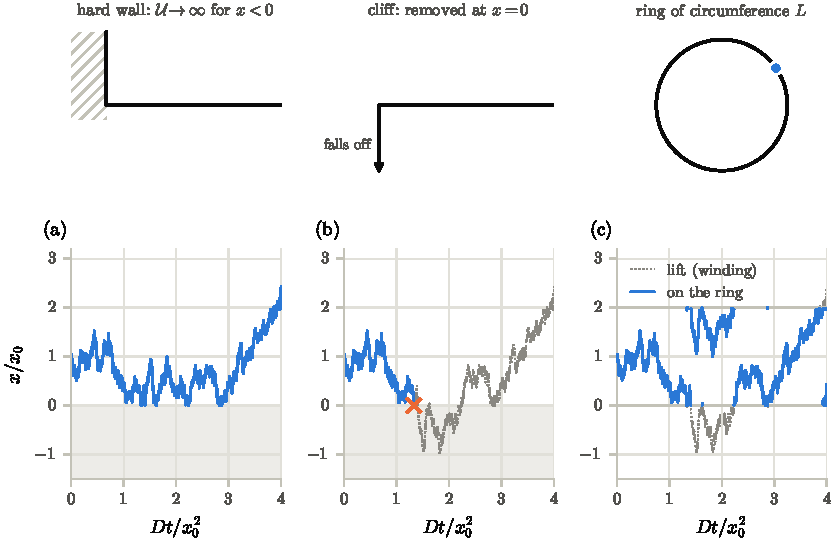
\includegraphics[width=\linewidth]{walls.pdf}
  \caption{Walls and domains as features of the landscape. Top: the potential. Bottom: one and the same Brownian
  path from $x_0$, treated three ways. (a)~A hard wall turns the path back; this is $|x|$, the image construction of
  \cref{sec:hl-reflecting}. (b)~At a cliff the path is removed at its first arrival (cross); the dotted
  continuation is what it would have done. (c)~On a ring of circumference $2x_0$ the path wraps around (solid);
  the dotted curve is its lift, which counts the windings (\cref{sec:circle-toolkit}).}
  \label{fig:walls}
\end{figure}

\begin{figure}[tbp]
  \centering
  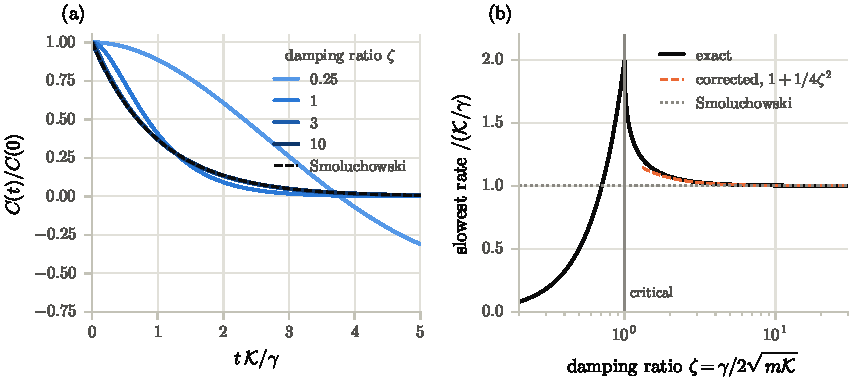
\includegraphics[width=\linewidth]{overdamped.pdf}
  \caption{A particle in a harmonic trap with inertia, against the overdamped (Smoluchowski, OU) description.
  (a)~Stationary position correlation for several damping ratios; dashed, the OU prediction $e^{-\mathcal Kt/\gamma}$.
  (b)~Long-time decay rate in units of the Smoluchowski rate $\mathcal K/\gamma$. It is largest, twice the Smoluchowski
  value, at critical damping. Dashed, Gardiner's corrected Smoluchowski equation \G{6.4.108}.}
  \label{fig:overdamped}
\end{figure}

\subsection{Stationary solution \texorpdfstring{\Gs{5.2.2}}{}}
\label{sec:stationary}

With zero current at both ends, the stationary equation integrates once to $J=0$ and once more to
Gardiner's potential solution \G{5.2.38}--\G{5.2.39},
\begin{equation}
  p_s(x)=\frac{\mathcal N}{B(x)}\exp\int^x\frac{2A(x')}{B(x')}\,\dd x'=\frac{\mathcal N\,\psi(x)}{B(x)},
  \label{eq:ps}
\end{equation}
with the same $\psi$ that appears in the first-passage formulas \G{5.2.44}, \G{5.2.157}. For the three drifts
of Parts I--III it gives a uniform density ($A=0$), the barometric $e^{2vx/D}$ ($A=v$), and the Gaussian
$e^{-kx^2/D}$ ($A=-kx$). A stationary state exists only if \cref{eq:ps} is normalisable \G{5.2.40}; on the
free half-line it is not.

\subsection{Eigenfunction expansion \texorpdfstring{\Gs{5.2.5}}{}}
\label{sec:eigen}

Gardiner's $P_\lambda(x)$ is an eigenfunction of the forward operator and $Q_\lambda(x)$ one of the backward
operator, with the same rate: $\mathcal LP_\lambda=-\lambda P_\lambda$ \G{5.2.75} and
$\mathcal L^\dagger Q_\lambda=-\lambda Q_\lambda$ \G{5.2.76} (the operators are \cref{eq:operators}). $P_\lambda$
is a density profile that decays as $e^{-\lambda t}$; $Q_\lambda$ is a function of the starting point. For a
time-independent problem with stationary solution $p_s$ (the reflecting one, even when the walls are absorbing
\G{5.2.91}), they are related by $P_\lambda = p_s\,Q_\lambda$ and normalised by
$\int P_\lambda Q_{\lambda'}\,\dd x=\int p_sQ_\lambda Q_{\lambda'}\,\dd x=\delta_{\lambda\lambda'}$
\G{5.2.79}--\G{5.2.80}, so that $P_0=p_s$ and $Q_0=1$ \G{5.2.82}--\G{5.2.83}. (The relation is \G{5.2.71} applied
to the solutions \G{5.2.73}--\G{5.2.74}.) Then
\begin{align}
  p(x,t\given x_0,0) &= \sum_\lambda P_\lambda(x)\,Q_\lambda(x_0)\,e^{-\lambda t}, && \G{5.2.88}\\
  \avg{x(t)x(0)}_s &= \sum_\lambda \Bigl[\int x\,P_\lambda(x)\,\dd x\Bigr]^2 e^{-\lambda t}. && \G{5.2.90}
\end{align}
With reflecting walls $\lambda=0$ is in the spectrum and $p\to p_s$; with absorbing walls it is not and
$p\to0$.

Every example's box names its $P_\lambda$ and $Q_\lambda$, normalised so that \G{5.2.88} holds as it stands.
Four situations go beyond Gardiner's \Gs{5.2.5}:
\begin{itemize}
  \item \textbf{Continuous spectrum.} On an unbounded domain the sum becomes an integral over a continuous label
        $k$, and $\delta_{\lambda\lambda'}$ becomes $\delta(k-k')$. Then $p_s$ is often not normalisable, and the
        weight in $P_\lambda=p_sQ_\lambda$ is the zero-current solution \cref{eq:ps}, fixed only up to a constant;
        the boxes say which constant.
  \item \textbf{Complex modes.} The pairing \G{5.2.79} is $\int P_\lambda Q_{\lambda'}$, with no complex
        conjugate, so a forward mode $e^{iqx}$ pairs with the backward mode $e^{-iqx}$.
  \item \textbf{A stationary current.} \G{5.2.71}--\G{5.2.72} need $J_s=0$. With a current (a circle with $\Phi\ne0$,
        or reinjection through infinity) $P_\lambda$ and $Q_\lambda$ have to be found separately. They are still
        biorthogonal \G{5.2.79}, but $P_\lambda\neq p_sQ_\lambda$.
  \item \textbf{Positive solutions off the spectrum.} Some QSDs solve the forward eigen-equation at a $\lambda$
        that is not in the spectrum: their partner $Q_\lambda=P_\lambda/p_s$ grows so fast that
        $\int P_\lambda Q_\lambda$ diverges (\cref{sec:drift-hl-absorbing,sec:ou-hl-absorbing,sec:sqrt}).
\end{itemize}

\subsection{Which operator, on which space}
\label{sec:operator}

Three things must be fixed before ``the spectrum'' means anything: the differential expression, the conditions
at the walls, and the space of functions it acts on. Change any one of them and the spectrum can change.

\paragraph{Two operators.} The forward (Fokker--Planck) operator acts on densities, and the backward operator on
functions of the starting point:
\begin{equation}
  \mathcal Lp=-\partial_x(Ap)+\tfrac12\partial_x^2(Bp)=-\partial_xJ,\qquad
  \mathcal L^\dagger f=A\,\partial_xf+\tfrac12B\,\partial_x^2f .
  \label{eq:operators}
\end{equation}
$\mathcal L^\dagger$ is what probabilists call the \emph{generator} of the process: the average $\avg{f(x(t))}$,
as a function of the start $x_0$, obeys $\partial_t\avg f=\mathcal L^\dagger\avg f$, as in \cref{eq:backward}.
The two operators are adjoint under the pairing $\int f\,p\,\dd x$, the average of $f$ over the density $p$.
Integrating by parts, as Gardiner does in \G{5.2.77},
\begin{equation}
  \int f\,\mathcal Lp\,\dd x-\int p\,\mathcal L^\dagger f\,\dd x
  =\Bigl[-f\,J-\tfrac12B\,p\,\partial_xf\Bigr]_{\text{walls}} ,
  \label{eq:green}
\end{equation}
where $J$ is the current of $p$.
\begin{itemize}
  \item \textbf{The walls are part of the operator.} The boundary terms vanish when the forward and backward
        conditions are paired: $J=0$ with $\partial_xf=0$ at a reflecting wall \G{5.2.69}, and $p=0$ with $f=0$
        at an absorbing one \G{5.2.67}. A circle has no walls, and no boundary terms. So the same differential
        expression with reflecting or with absorbing walls is a different operator, with a different spectrum
        (\cref{sec:reflecting,sec:absorbing}). In operator language, the wall conditions specify the
        \emph{domain}.
  \item \textbf{What the eigenvalues belong to.} Gardiner's eigen-equations \G{5.2.75}--\G{5.2.76} are
        $\mathcal LP_\lambda=-\lambda P_\lambda$ and $\mathcal L^\dagger Q_\lambda=-\lambda Q_\lambda$. Every
        $\lambda$ in these notes is an eigenvalue of $-\mathcal L$ and, with the paired walls, of
        $-\mathcal L^\dagger$. \Cref{eq:green} with $p=P_\lambda$ and $f=Q_{\lambda'}$ gives
        $(\lambda'-\lambda)\int P_\lambda Q_{\lambda'}\,\dd x=0$, the biorthogonality \G{5.2.79}.
  \item \textbf{Conservation.} With no absorbing wall, $f=1$ satisfies the backward condition and
        $\mathcal L^\dagger1=0$, so $Q_0=1$ \G{5.2.83} always exists. Its forward partner $P_0=p_s$ \G{5.2.82}
        exists only if it is normalisable. That is the question in the first item of
        \cref{sec:spectrum-states}.
\end{itemize}

\paragraph{Three spaces.} Each answers a different question (\cref{tab:spaces}).
\begin{table}[h]
\centering
\small
\renewcommand{\arraystretch}{1.3}
\begin{tabular}{@{}l l l l@{}}
\toprule
Space & Contains & Operator & Used for \\
\midrule
$L^1$ & densities, $\int|p|\,\dd x<\infty$ & $\mathcal L$ & probability; stationary states and QSDs \\
$L^2(1/p_s)$ & $\int p^2/p_s\,\dd x<\infty$ & $\mathcal L$, self-adjoint if $J_s=0$ & real spectra, gaps, expansions, bounds \\
$L^\infty$ & bounded observables $f(x_0)$ & $\mathcal L^\dagger$ & $S(t\given x_0)$, $T(x_0)$, $\pi_a$, $\pi_b$ \\
\bottomrule
\end{tabular}
\caption{The spaces on which the operators \cref{eq:operators} act.}
\label{tab:spaces}
\end{table}
\begin{itemize}
  \item \textbf{$L^1$ is where probability lives.} The forward evolution keeps densities positive and never
        increases $\int|p|$; with no absorption it conserves $\int p$. Stationary states and QSDs are, by
        definition, positive eigenfunctions in $L^1$.
  \item \textbf{$L^\infty$ is its dual,} where the backward evolution acts on observables. The survival
        probability is the backward evolution of $f=1$ with absorbing walls, and all the first-passage functions
        of \cref{sec:fpt-toolkit} are backward objects.
  \item \textbf{$L^2(1/p_s)$ is where the operator is self-adjoint.} It is the only one of the three with an inner
        product, so it is where orthogonality, eigenfunction expansions and variational bounds live. Gardiner's
        substitution $p=p_sq$ \G{5.2.71} turns the forward operator into the backward one,
        $\mathcal L(p_sq)=p_s\mathcal L^\dagger q$ \G{5.2.72}, whenever the stationary current vanishes. Then
        \cref{eq:green} becomes
        \begin{equation}
          \int\frac{g\,\mathcal Lp}{p_s}\,\dd x=\int\frac{p\,\mathcal Lg}{p_s}\,\dd x,\qquad
          -\int\frac{p\,\mathcal Lp}{p_s}\,\dd x=\tfrac12\int B\,p_s\Bigl[\partial_x\frac{p}{p_s}\Bigr]^2\dd x\;\ge0 .
          \label{eq:dirichlet}
        \end{equation}
        So $-\mathcal L$ is self-adjoint and non-negative: $\lambda$ is real and $\ge0$, the orthogonality
        relations \G{5.2.80}--\G{5.2.81} hold, and the right-hand side is the numerator of the Rayleigh quotient
        \cref{eq:rayleigh}. The weight need not be normalisable. It is the zero-current solution
        $p_s=\psi/B$ of \cref{eq:ps}, which exists on any interval or line: the free half-line uses $p_s=1$, and
        absorbing problems use the $p_s$ of the same problem with reflecting walls \G{5.2.91}.
\end{itemize}
On a bounded domain the eigenfunctions are smooth and bounded, so all three spaces give the same discrete
spectrum. On an unbounded domain they need not agree. The continua of QSDs in \cref{sec:spectrum-states} are
eigenvalues in $L^1$ that are not in the $L^2$ spectrum, and probability escaping to infinity is visible in $L^1$
but not in $L^2$.

\paragraph{Discrete and continuous spectrum.} $\lambda$ is an eigenvalue when its eigenfunction lies in the space.
On an unbounded domain there is also continuous spectrum, made of generalised eigenfunctions that are bounded
but not normalisable, such as $e^{ikx}$ on the line. The sum \G{5.2.88} then becomes an integral over $k$, as in
\cref{sec:line,sec:hl-reflecting,sec:hl-absorbing}.

\paragraph{The symmetrised form: a Schr\"odinger operator.} The weight can be absorbed into the function. With
$B=D$, write $p=\sqrt{p_s}\,\psi$, so that $\int p^2/p_s\,\dd x=\int\psi^2\,\dd x$. Then $\partial_tp=\mathcal Lp$
becomes
\begin{equation}
  \partial_t\psi=-H\psi,\qquad H=-\tfrac12D\,\partial_x^2+V(x),\qquad V=\frac{A^2}{2D}+\frac{A'}{2},
  \label{eq:schrodinger}
\end{equation}
a Schr\"odinger operator in plain $L^2$, with $D$ in the role of $\hbar^2/m$. Its spectrum is the
$L^2(1/p_s)$ spectrum of $-\mathcal L$, and its ground state at $\lambda=0$ is $\sqrt{p_s}$ when that is
normalisable. If $\psi_\lambda$ are its orthonormal eigenfunctions, Gardiner's are
\begin{equation}
  P_\lambda=\sqrt{p_s}\,\psi_\lambda,\qquad Q_\lambda=\psi_\lambda/\sqrt{p_s},
  \label{eq:PQ-psi}
\end{equation}
which satisfy $P_\lambda=p_sQ_\lambda$ and $\int P_\lambda Q_{\lambda'}=\int\psi_\lambda\psi_{\lambda'}=\delta_{\lambda\lambda'}$
at once; the constant in a non-normalisable $p_s$ cancels from every product $P_\lambda(x)Q_\lambda(x_0)$. The walls become
\begin{equation}
  \text{absorbing: }\psi=0,\qquad \text{reflecting: }\partial_x\psi=\frac{A}{D}\,\psi .
  \label{eq:schrodinger-walls}
\end{equation}
\begin{itemize}
  \item \textbf{Reading the spectrum off $V$.} A bounded domain, or $V\to\infty$ at infinity, gives a discrete
        spectrum. Otherwise the continuum starts at the limit of $V$ at infinity: that is where the edges of
        \cref{sec:gap} come from.
  \item \textbf{Part~I:} $V=0$, a free particle, with Dirichlet or Neumann walls.
  \item \textbf{Part~II:} $V=v^2/2D=1/2\tau$, a constant. The gauge \cref{eq:gauge} is exactly this
        symmetrisation, since $\sqrt{p_s}\propto e^{\alpha x}$. The constant potential is the shift $1/2\tau$
        of every rate, and the Robin condition $u'=\alpha u$ of \cref{sec:drift-gauge} is
        \cref{eq:schrodinger-walls} with $A=v$. On the half-line the continuum starts at
        $V(\infty)=1/2\tau$.
  \item \textbf{Part~III:} $V=\tfrac12k(\xi^2-1)$, a harmonic oscillator whose zero-point energy $k/2$ is
        cancelled, so $\lambda=nk$ with $\psi_n\propto H_n(\xi)e^{-\xi^2/2}$. A wall at the bottom keeps the even
        states (reflecting, $\psi'=0$) or the odd ones (absorbing, $\psi=0$) (\cref{fig:operators}a).
  \item \textbf{Circles.} Near an extremum of $U$, $A\approx0$ and $V\approx A'/2=-U''/2$, and the $A^2$ term
        grows away from it. So in a deep enough well both the bottom and the top of $U$ are wells of $V$.
        \begin{itemize}
          \item The smooth cosine well (\cref{sec:cos-circle}) has two wells in $V$, offset by $k$, and each
                nonzero level has one copy in each, of opposite parity (\cref{fig:operators}b). These are the
                doublets.
          \item The sawtooth (\cref{sec:ou-circle}) has a single harmonic well, plus a repulsive spike
                $\tfrac12kL\,\delta$ at the cusp, where $A'$ jumps. Its levels are single
                (\cref{fig:operators}c).
        \end{itemize}
  \item \textbf{With a current} (on a circle with nonzero circulation $\Phi=\oint2A/B$,
        \cref{sec:circle-toolkit}) there is no zero-current $p_s$ to symmetrise with. In
        plain $L^2$ the drift term $-v\partial_x$ is anti-self-adjoint, which is why the eigenvalues of
        \cref{sec:drift-circle} have imaginary parts $\pm vq_m$. The operator is still normal, with orthogonal
        Fourier modes, and biorthogonality \G{5.2.79} holds with $P_m=e^{iq_mx}/L$ and $Q_m=e^{-iq_mx}$.
\end{itemize}

\begin{figure}[tbp]
  \centering
  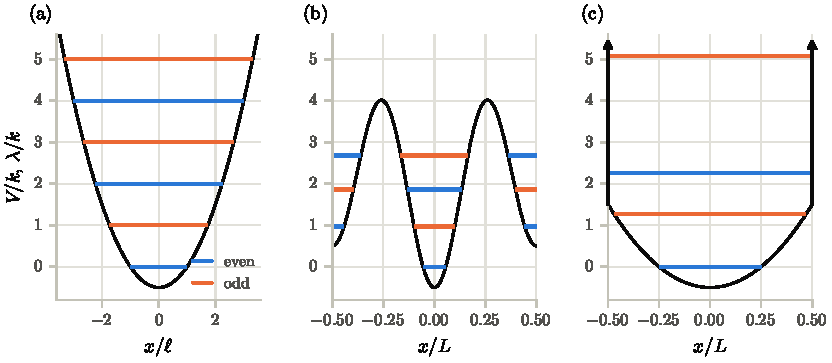
\includegraphics[width=\linewidth]{operators.pdf}
  \caption{Symmetrised potentials $V=A^2/2D+A'/2$ (black) and their levels, drawn where $V<\lambda$, in units
  of $k$. Blue levels are even under $x\to-x$, orange ones odd.
  (a)~OU on the line: a harmonic oscillator with levels $nk$. A wall at the bottom keeps one parity.
  (b)~The cosine well on a circle, $\kappa=16$: $V$ has a well at the bottom of $U$ ($x=0$) and one at its top
  ($x=\pm L/2$). Each nonzero level has a copy in each well, of opposite parity.
  (c)~The sawtooth on a circle, $L=4\ell$: one harmonic well and a $\delta$-function spike at the cusp (arrows).
  The levels are single, in pairs split by exactly $k$.}
  \label{fig:operators}
\end{figure}

\subsection{The spectral gap}
\label{sec:gap}

Most long-time statements in these notes come from one property of this expansion. Order the eigenvalues
$\lambda_{\min}<\lambda_{\text{next}}<\cdots$. With reflecting or absorbing walls, or on a circle without a
current, the operator is self-adjoint with respect to the weight $1/p_s$ (\Gs{5.2.5}; \cref{sec:operator}), so the
eigenvalues are real and non-negative and the eigenfunctions are complete. (Each section labels modes by their natural quantum number, so the lowest one
may be called $\lambda_0$ or $\lambda_1$. What matters is lowest and next-lowest.)

\paragraph{What the gap is.} Keep the two slowest terms of \G{5.2.88}:
\begin{equation}
  p(x,t\given x_0,0)=P_{\min}(x)\,Q_{\min}(x_0)\,e^{-\lambda_{\min}t}
  +P_{\text{next}}(x)\,Q_{\text{next}}(x_0)\,e^{-\lambda_{\text{next}}t}+\cdots
  \label{eq:gap-expansion}
\end{equation}
\begin{itemize}
  \item \textbf{Reflecting or confining problems} have $\lambda_{\min}=0$, with $P_{\min}=p_s$ and $Q_{\min}=1$.
        Then $p-p_s\approx P_{\text{next}}Q_{\text{next}}(x_0)\,e^{-\lambda_{\text{next}}t}$: the distance from
        equilibrium decays at $\lambda_{\text{next}}$. The \emph{spectral gap} is
        $\lambda_{\text{next}}-\lambda_{\min}=\lambda_{\text{next}}$, and its inverse is the relaxation time.
        Every expectation value, and every stationary correlation function
        $C(\tau)=\sum_nc_n^2e^{-\lambda_n\tau}$ \G{5.2.90}, ends up decaying at the gap.
  \item \textbf{Absorbing problems} have $\lambda_{\min}>0$. Then $\lambda_{\min}$ is the decay rate of the
        survival probability, $S\propto e^{-\lambda_{\min}t}$, and the conditioned density $q=p/S$ tends to the
        QSD $\propto P_{\min}$. The gap $\lambda_{\text{next}}-\lambda_{\min}$ sets how fast $q$ forgets where
        it started: $q-q_\infty\propto e^{-(\lambda_{\text{next}}-\lambda_{\min})t}$. On an unbounded domain
        this holds for localised starts; a heavy-tailed start can reach a different QSD
        (\cref{sec:spectrum-states}).
  \item \textbf{Selection by symmetry.} If an initial condition or observable has no overlap with the next
        mode, it relaxes at the next rate it does overlap. Examples: starting at the centre of a symmetric
        interval (\cref{sec:reflecting,sec:absorbing}), and $\avg{x^2}$ in the Ornstein--Uhlenbeck process
        (\cref{sec:ou-line}).
\end{itemize}

\paragraph{Why the gap has the size it does.} With zero-current walls, $\lambda_{\text{next}}$ is the minimum
of a Rayleigh quotient over functions with $\int p_sf=0$:
\begin{equation}
  \lambda_{\text{next}}=\min_f\frac{\tfrac12\int B\,p_s\,(f')^2\,\dd x}{\int p_s\,f^2\,\dd x}
  \qquad\text{(Poincar\'e inequality)}.
  \label{eq:rayleigh}
\end{equation}
A small gap needs a function that is not constant but costs little gradient, weighted by $p_s$:
\begin{itemize}
  \item a long domain lets $f$ vary slowly, at cost $\sim D/L^2$, so $\lambda\approx\pi^2D/2L^2$
        (\cref{sec:reflecting});
  \item a barrier lets $f$ be nearly $+1$ on one side and $-1$ on the other, changing only where $p_s$ is
        exponentially small, so the rate is exponentially small (Arrhenius, \cref{sec:drift-mixed,sec:ou-mixed});
  \item confinement works the other way. A restoring force concentrates $p_s$ and keeps the gap finite even
        on an infinite domain (the Ornstein--Uhlenbeck gap $k$, \cref{sec:ou-line}).
\end{itemize}

\paragraph{Discrete levels, continua, and no gap.}
\begin{itemize}
  \item Bounded domains, and confining forces, give discrete spectra: the gap is positive and relaxation is
        exponential.
  \item An unbounded domain without confinement gives a continuous spectrum down to $\lambda=0$: there is no
        gap, and relaxation is algebraic (the $t^{-1/2}$ of \cref{sec:hl-absorbing}).
  \item A continuum can start above zero, as with drift toward a wall on the half-line
        (\cref{sec:drift-hl-absorbing}). Its edge plays the role of the gap, but the approach carries an
        algebraic prefactor ($t^{-3/2}$).
  \item Isolated levels below a continuum (bound states) appear when a force pushes against a reflecting
        wall: the stationary state of \cref{sec:drift-hl-reflecting}, or the Arrhenius level of
        \cref{sec:drift-mixed}.
  \item Symmetry can make levels degenerate. On a circle the nonzero levels of a reflection-symmetric
        problem come in doublets (\cref{sec:circle}). With a circulating current they become complex-conjugate
        pairs and the density spirals as it relaxes; the gap is then $\operatorname{Re}\lambda$
        (\cref{sec:drift-circle}).
\end{itemize}
\Cref{fig:spectra} shows these cases side by side.

\paragraph{Caveat.} With drift, the operator is self-adjoint only with the weight. In ordinary distance the
slowest mode can take a transit time to dominate (\cref{sec:drift-gauge}). The gap gives the asymptotic rate,
not the length of the transient.

\begin{figure}[tbp]
  \centering
  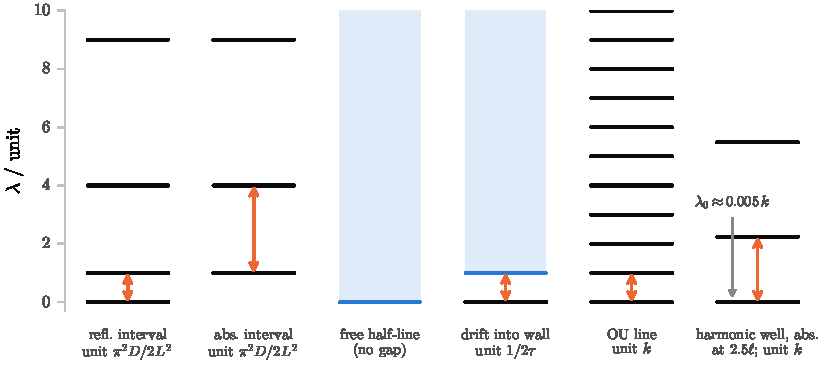
\includegraphics[width=\linewidth]{spectra.pdf}
  \caption{Spectra of six examples, each in its own natural rate. Ticks are discrete eigenvalues, shaded
  bands continua, and the arrow is the gap that controls the long-time behaviour. For the absorbing interval
  the lowest level is the decay rate of $S$, and the arrow is the rate of convergence to the QSD. The last
  column is the harmonic well with a reflecting wall at its bottom and an absorbing wall at $L=2.5\ell$
  (\cref{sec:ou-mixed}); its lowest level, $\approx0.005\,k$, is the Kramers escape rate.}
  \label{fig:spectra}
\end{figure}

\subsection{First passage \texorpdfstring{\Gs{5.2.7}--\Gs{5.2.8}}{}}
\label{sec:fpt-toolkit}

For walls $a<b$, both absorbing, and a start at $x_0$ (see also Redner~\cite{redner}, ch.~2):
\begin{itemize}
  \item \textbf{Survival} $S(t\given x_0)=\int_a^b p(x,t\given x_0,0)\,\dd x=\Pr(T>t)$; this is Gardiner's
        $G(x_0,t)$ \G{5.2.140}. It obeys the backward equation with $S(x_0,0)=1$, $S(a,t)=S(b,t)=0$.
  \item \textbf{Exit-time density} $f(t)=-\partial_tS = j_a(t)+j_b(t)$, with outward fluxes
        $j_a=-J(a,t)$, $j_b=J(b,t)$.
  \item \textbf{Moments} $T_k(x_0)=\avg{T^k}=k\int_0^\infty t^{k-1}S\,\dd t$ satisfy
        $A\,T_k'+\tfrac12B\,T_k''=-k\,T_{k-1}$, $T_0=1$, $T_k(a)=T_k(b)=0$ \G{5.2.154}, \G{5.2.156}.
        With $\psi(x)=\exp\int^x 2A/B$, $T_1$ is given in closed form by \G{5.2.157}--\G{5.2.158}.
  \item \textbf{Splitting probabilities} $\pi_a+\pi_b=1$, with $A\pi_a'+\tfrac12B\pi_a''=0$, $\pi_a(a)=1$,
        $\pi_a(b)=0$ \G{5.2.186}--\G{5.2.187}. The solution is
        $\pi_b(x)=\int_a^x\dd y/\psi(y)\big/\int_a^b\dd y/\psi(y)$, since $\pi'\propto1/\psi$.
        \textbf{Misprint:} \G{5.2.189}--\G{5.2.190} as printed in the 2nd edition have $\psi$ in place of
        $1/\psi$. That gives the wrong sign of the drift dependence; it only matters once $A\neq0$.
  \item \textbf{Conditional mean exit times} $T_a(x_0)=\avg{T\given\text{exit at }a}$ from
        $A(\pi_aT_a)'+\tfrac12B(\pi_aT_a)''=-\pi_a$, $\pi_aT_a=0$ at both walls \G{5.2.183}. Check:
        $\pi_aT_a+\pi_bT_b=T_1$.
  \item \textbf{Conditioned density} $q=p/S$ obeys $\partial_tq=\mathcal Lq+\kappa(t)q$ with exit rate
        $\kappa=-\dot S/S=f/S$. Its fixed points are the quasi-stationary distributions (QSDs). On a bounded
        domain there is exactly one, the positive ground state $\phi_1$ of $\mathcal L\phi=-\lambda\phi$ with
        absorbing walls, and $\kappa\to\lambda_1$ \cite{collet}. On an unbounded domain there can be none or
        a continuum (\cref{sec:spectrum-states}).
\end{itemize}

\subsection{Stationary states and QSDs from the spectrum}
\label{sec:spectrum-states}

A stationary state is a positive, integrable solution of $\mathcal L\phi=0$. A QSD is a positive, integrable
solution of $\mathcal L\phi=-\lambda\phi$ with $\lambda>0$ that vanishes at the absorbing walls~\cite{collet}.
Neither definition mentions the spectrum. How much does the spectrum used in these notes reveal? That is the
spectrum in $L^2(1/p_s)$, where the operator is self-adjoint (\cref{sec:operator}); in Part~II it is the
spectrum of the gauged problem.

\paragraph{Bounded domains: everything.} The spectrum is discrete, and the lowest eigenfunction is the only
positive one: every other eigenfunction is orthogonal to the positive ground state of the backward problem
(for a conservative problem, $\int P_n\,\dd x=0$), so it must change sign.
\begin{itemize}
  \item With no absorption the lowest eigenvalue is $0$, its eigenfunction is the unique stationary state, and
        every start converges to it at the gap. This includes the circle with a current
        (\cref{sec:drift-circle}), whose other eigenvalues are complex while $0$ stays isolated.
  \item With absorption the lowest eigenvalue $\lambda_{\min}>0$ is the decay rate of $S$, its eigenfunction
        is the unique QSD, and every start converges to it at rate $\lambda_{\rm next}-\lambda_{\min}$.
\end{itemize}

\paragraph{Stationary states never form a continuum.} On a connected domain with $B>0$ the process can get
from anywhere to anywhere, and then it has at most one stationary state. It exists exactly when the stationary
solution \cref{eq:ps} is normalisable \G{5.2.40} (\cref{eq:circle-ps} on a circle). The continua below are all
of QSDs.

\paragraph{Unbounded domains: three things to check.}
\begin{enumerate}
  \item \textbf{Eigenvalue, or edge of a continuum.} If the bottom of the spectrum is the edge of a continuum
        and not an eigenvalue, there is no stationary state or QSD in $L^2$, and the approach is algebraic. The
        free line and half-lines are examples (\cref{sec:line,sec:hl-reflecting,sec:hl-absorbing}): their
        would-be eigenfunctions $1$ and $x$ are not normalisable. Conversely, $0$ can be an eigenvalue at the
        bottom of a continuum. Then $p_s$ exists but relaxation is slower than exponential. That happens when
        $p_s$ has power-law tails, which none of the examples here do; in one dimension a gap needs tails of
        $p_s$ that decay at least exponentially.
  \item \textbf{$L^2$ sees only local decay.} The weighted norm does not notice probability running off to
        infinity.
        \begin{itemize}
          \item Drift away from a reflecting wall (\cref{sec:drift-hl-reflecting}, $v>0$): the spectrum is
                $[1/2\tau,\infty)$, with no $0$, although probability is conserved. $1/2\tau$ is the rate at
                which the density at a fixed $x$ drops as the bulk drifts away.
          \item An absorbing wall with the drift toward it or away from it (\cref{sec:drift-hl-absorbing}): the
                spectrum is $[1/2\tau,\infty)$ for both signs, since the shift $v^2/2D$ is even in $v$. Yet
                toward the wall $S\sim t^{-3/2}e^{-t/2\tau}$, and away from it $S\to1-e^{-2x_0/\ell}$.
        \end{itemize}
  \item \textbf{Positive solutions below the bottom.} For these one-dimensional problems, positive solutions of
        $\mathcal L\phi=-\lambda\phi$ satisfying the wall condition exist exactly for $\lambda$ up to the bottom
        $\lambda_{\rm b}$ of the $L^2$ spectrum (in Schr\"odinger language, the Allegretto--Piepenbrink
        theorem). Below $\lambda_{\rm b}$ they are not in $L^2$, but they can still be integrable, and then they
        are QSDs (\cref{tab:spectrum-states}).
\end{enumerate}

\begin{table}[h]
\centering
\small
\renewcommand{\arraystretch}{1.3}
\begin{tabular}{@{}l l l l@{}}
\toprule
Absorbing problem & Bottom $\lambda_{\rm b}$ of $L^2$ spectrum & Positive, integrable $\phi$ & QSDs \\
\midrule
interval, \cref{sec:absorbing}                          & $\pi^2D/2L^2$, isolated & only at $\lambda_{\rm b}$ & one \\
free half-line, \cref{sec:hl-absorbing}                 & $0$, edge               & none ($\phi=x$)           & none \\
drift toward the wall, \cref{sec:drift-hl-absorbing}    & $1/2\tau$, edge         & every $\lambda\in(0,1/2\tau]$ & a continuum \\
drift away from the wall, \cref{sec:drift-hl-absorbing} & $1/2\tau$, edge         & none ($\phi$ grows)       & none: escape \\
OU, wall at the bottom, \cref{sec:ou-hl-absorbing}      & $k$, isolated           & every $\lambda\in(0,k]$   & a continuum \\
\bottomrule
\end{tabular}
\caption{How many QSDs each absorbing problem has.}
\label{tab:spectrum-states}
\end{table}

The last row shows that a discrete spectrum with an isolated bottom does not make the QSD unique on an
unbounded domain.

\paragraph{Uniqueness.} A theorem of Cattiaux et al.~\cite{cattiaux} gives the sharp criterion: there is
exactly one QSD, and it attracts every initial condition, if and only if $+\infty$ is an \emph{entrance}
boundary, meaning the process comes down from infinity in finite mean time. Equivalently, the mean absorption
time $T(x_0)$ of \cref{sec:fpt-toolkit} stays bounded as $x_0\to\infty$.
\begin{itemize}
  \item Bounded domains pass trivially.
  \item On the half-line, $T=x_0/|v|$ for drift toward the wall and $T\simeq\tau\ln(2x_0/\ell)$ for OU
        (\cref{sec:ou-hl-absorbing}) both grow without bound, hence the continua.
  \item A drift such as $A=-kx^3$, for which $T$ stays bounded, would have a unique QSD.
\end{itemize}

\paragraph{Which QSD is reached.} With a continuum, the initial condition decides, through its tail
(\cref{fig:attraction}).
\begin{itemize}
  \item \textbf{Point starts}, and anything localised enough, reach the \emph{minimal} QSD, the one at
        $\lambda_{\rm b}$ (the Yaglom limit). Through the gauge (Part~II) or the map (Part~III) the problem
        becomes the free absorbing half-line, whose density at large $t$ is $\propto x$ near the wall
        (\cref{sec:hl-absorbing}). Transformed back, that $x$ becomes the minimal QSD.
  \item \textbf{Heavy tails} change the outcome. Particles that start far out keep arriving at the wall long
        after the bulk has been absorbed. If the initial tail delivers survivors more slowly than
        $e^{-\lambda_{\rm b}t}$, they dominate, and the conditioned density settles on the QSD with the same
        tail and a smaller $\lambda$. In the free variables, the far-out part of the start contributes a profile
        that does not spread and decays more slowly than the minimal one
        (\cref{sec:drift-hl-absorbing,sec:ou-hl-absorbing}).
  \item The thresholds are sharp.
        \begin{itemize}
          \item Drift toward the wall: an initial tail $e^{-\beta x}$ with $\beta<1/\ell$ selects
                $\lambda=\beta|v|-\tfrac12D\beta^2$.
          \item OU: a tail $x^{-1-\nu}$ with $0<\nu<1$ (infinite mean) selects $\lambda=\nu k$.
          \item Lighter tails give the minimal QSD.
          \item Tails heavier than every exponential (drift) or every power (OU) give $\lambda\to0$. There the
                family is not normalisable, and the conditioned density never settles.
        \end{itemize}
\end{itemize}

\begin{figure}[tbp]
  \centering
  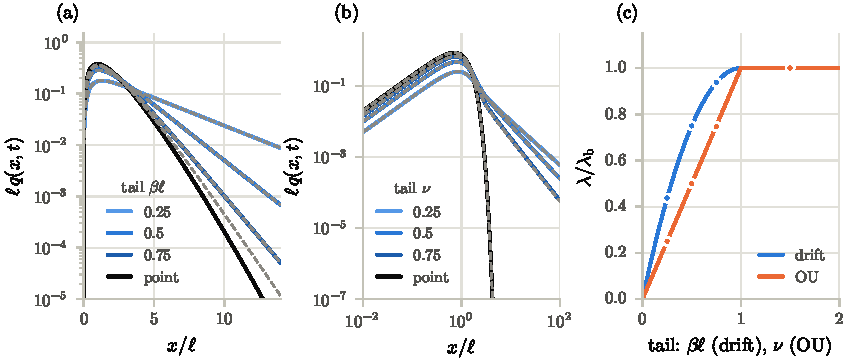
\includegraphics[width=\linewidth]{qsd_attraction.pdf}
  \caption{Which QSD a start reaches.
  (a)~Drift toward an absorbing wall: conditioned densities at $t=60\,\tau$ from exponential starts
  $\beta e^{-\beta x}$ and from a point start at $x_0=\ell$. Dashed, the QSDs with the same tails, and the edge
  QSD $xe^{-x/\ell}/\ell^2$, which the point start is still approaching, algebraically.
  (b)~OU with an absorbing wall at the bottom: conditioned densities at $t=12\,\tau$ from starts with tails
  $x^{-1-\nu}$, and from a point start at $x_0=2\ell$. Dashed, the QSDs $q_\nu$ and the Rayleigh density.
  (c)~Decay rate of $S$ selected by the initial tail, in units of $\lambda_{\rm b}$ ($1/2\tau$ for drift, $k$ for
  OU). Curves are the predictions; dots are measured from the exact evolution.}
  \label{fig:attraction}
\end{figure}

\subsection{Periodic boundaries: the circle}
\label{sec:circle-toolkit}

Gardiner treats periodic boundaries \Gs{5.2.1d} by taking an interval $[a,b]$, identifying its ends, and requiring
\begin{equation*}
  \lim_{x\to b^-}p=\lim_{x\to a^+}p\quad\G{5.2.17},\qquad \lim_{x\to b^-}J=\lim_{x\to a^+}J\quad\G{5.2.18}.
\end{equation*}
These are borrowed from his conditions at a discontinuity of the coefficients, \G{5.2.15}--\G{5.2.16}, so $A$
and $B$ are allowed to jump at the seam; that they do not, \G{5.2.19}, is presented as the most frequent case.
The stationary solution \G{5.2.41}--\G{5.2.47} is then written relative to the seam, through $p_s(a)$ and
integrals that start at $a$.

These notes take the topology at face value instead. The state space is the circle $S^1=\mathbb R/L\mathbb Z$,
of circumference $L$ and radius $R=L/2\pi$. A circle has no boundary, so there is nothing to impose and no
special point.
\begin{itemize}
  \item $A$, $B$ and $p$ are functions on the circle, that is, $L$-periodic functions on $\mathbb R$, with the
        same smoothness at every point. A coordinate needs a cut somewhere, but no result may depend on where
        the cut is, and every formula below is invariant under moving it.
  \item \G{5.2.17}--\G{5.2.18} are not boundary conditions. Continuity of $p$ and $J$ holds at every point,
        because $\partial_tp=-\partial_xJ$ needs it, and at the ``seam'' it holds for the same reason as
        anywhere else. A genuine discontinuity of $A$ or $B$ is a property of the coefficients at that point;
        \G{5.2.15}--\G{5.2.16} then apply there, wherever it is (\cref{sec:ou-circle}).
  \item Probability is conserved because the circle has no boundary,
        $\frac{\dd}{\dd t}\oint p\,\dd x=-\oint\partial_xJ\,\dd x=0$, not because two currents happen to match.
        The backward equation needs no condition either: the surface term \G{5.2.65}, which produces
        \G{5.2.67} and \G{5.2.69}, is absent.
  \item Observables must be functions on the circle too. The coordinate $x$ is not one, since it jumps at the
        cut, so $\avg x$ and the correlation function \G{5.2.90} depend on where the cut is. The natural
        observables are the Fourier modes $e^{iq_mx}$, $q_m=2\pi m/L$.
\end{itemize}

\paragraph{The universal cover.} The map $\mathbb R\to S^1$, $\tilde x\mapsto\tilde x\bmod L$, unwraps the
circle. A path on the circle lifts to a unique path $\tilde x(t)$ on $\mathbb R$ once its starting point is
lifted, and the lift obeys the same Fokker--Planck equation with the coefficients repeated periodically.
Summing over where the lift can end,
\begin{equation}
  p_{S^1}(x,t\given x_0,0)=\sum_{n\in\mathbb Z}p_{\mathbb R}(x+nL,t\given x_0,0).
  \label{eq:cover}
\end{equation}
This is the method of images for the group of translations by $L$, and every image enters with a plus sign.
A mirror imposes a condition, which is why images could change sign on the intervals; a translation imposes
nothing, it is just another way of arriving at the same point.

\paragraph{Winding.} The lift gives the circle an observable that no interval has: the unwrapped displacement
$\Delta\tilde x(t)=\tilde x(t)-\tilde x(0)$, the net distance travelled around the circle. It exists because
the circle contains a loop that cannot be shrunk to a point. Its long-time drift and spread,
\begin{equation}
  \avg{\Delta\tilde x}\simeq v_{\rm w}t,\qquad \operatorname{Var}\Delta\tilde x\simeq D_{\text{eff}}\,t,
  \label{eq:winding}
\end{equation}
are the transport coefficients of the circle: the winding velocity $v_{\rm w}$ and the effective diffusion
constant.
\begin{itemize}
  \item $v_{\rm w}=\oint J\,\dd x=LJ_s$: the stationary current is the winding rate.
  \item Let $T_{\rm w}(x_0)$ be the mean time for the lift to first get a full circumference from its start,
        either way: the exit time from $(x_0-L,x_0+L)$ on the cover, an absorbing-interval problem
        \G{5.2.158}. After each such event the process starts afresh at an equivalent point, so the windings
        form a random walk with steps $\pm L$. If $v_{\rm w}=0$, the renewal theorem gives $D_{\rm eff}=L^2/T_{\rm w}$;
        in particular $T_{\rm w}$ is then the same from every starting point.
  \item Both coefficients also follow from one eigenvalue. $\avg{e^{s\Delta\tilde x}}\sim e^{\Lambda(s)t}$,
        where $\Lambda(s)$ is the top eigenvalue of the generator with $\partial_x\to\partial_x-s$, acting on
        periodic functions; then $v_{\rm w}=\Lambda'(0)$ and $D_{\rm eff}=\Lambda''(0)$. The script computes both this
        way, by perturbation theory in $s$.
\end{itemize}

\paragraph{Stationary state and current.} Let $\varphi(x)=\int^x2A/B$ on the cover, so that $\psi=e^\varphi$
is Gardiner's \G{5.2.44}, and let
\begin{equation}
  \Phi=\oint\frac{2A}{B}\,\dd x=\varphi(x+L)-\varphi(x),
\end{equation}
which does not depend on $x$. Integrate $J={}$const as in \G{5.2.45}, but once around the loop from $x$ back to
itself rather than from a seam:
\begin{equation}
  p_s(x)=\frac{\mathcal N}{B(x)}\int_x^{x+L}e^{\varphi(x)-\varphi(y)}\,\dd y,\qquad
  J_s=\frac{\mathcal N}{2}\bigl(1-e^{-\Phi}\bigr),
  \label{eq:circle-ps}
\end{equation}
with $\mathcal N$ fixed by $\oint p_s=1$. This is \G{5.2.47}, rewritten so that the only point it refers to is
$x$ itself; the script checks that the two agree.
\begin{itemize}
  \item \textbf{Detailed balance is topological.} $J_s=0$ exactly when $\Phi=0$, that is, when $2A/B$ is the
        derivative of a function on the circle, a single-valued potential. Then $\psi$ is a function on the
        circle and \cref{eq:circle-ps} reduces to the potential solution \cref{eq:ps}. If $\Phi\neq0$ a current
        with the sign of $\Phi$ circulates forever: a non-equilibrium steady state (NESS). Adding a periodic
        potential to $A$ changes how large $J_s$ is, but never whether it vanishes.
  \item \textbf{Misprint.} \G{5.2.46} as printed reads
        $J=[B(b)/\psi(b)-B(a)/\psi(a)]\,p_s(a)\big/\!\int_a^b\dd x/\psi$. Setting $x=b$ in \G{5.2.45} and using
        $p_s(b)=p_s(a)$ gives instead $J=[B(a)/\psi(a)-B(b)/\psi(b)]\,p_s(a)\big/2\!\int_a^b\dd x/\psi$: the sign
        is reversed and a factor $\tfrac12$ is missing. For constant drift the printed form gives $J=-2v/L$
        instead of $v/L$ (\cref{sec:drift-circle}). \G{5.2.47} is correct.
\end{itemize}

\paragraph{Spectrum.} If $\Phi=0$ the operator is self-adjoint with weight $1/p_s$ and \Gs{5.2.5} applies
unchanged, with $Q$ periodic. If $\Phi\neq0$ no weight makes it self-adjoint, and eigenvalues can come in
complex-conjugate pairs: probability circulates while it relaxes. The gap is then the smallest nonzero
$\operatorname{Re}\lambda$.

\paragraph{Folding.} A reflection of the circle fixes two antipodal points, $c$ and $c+L/2$. If $B$ is even and
$A$ odd under it, the problem splits into an even sector and an odd sector. Even densities have $J=0$ at both
fixed points and odd ones have $p=0$ there, so the even sector is the interval $(c,c+L/2)$ with reflecting
walls and the odd sector the same interval with absorbing walls. This is how the circle connects to the
intervals.

\paragraph{First passage.} A point becomes special only when a question makes it special. To find when the
process first reaches a target $c$, cut the circle there. It becomes the interval $(c,c+L)$ with both ends
absorbing, the two ends being the target approached from either side, and the splitting probabilities say
which way round the particle arrived. The first full winding, likewise, is the absorbing interval
$(x_0-L,x_0+L)$ on the cover.

\subsection{How the notes are built}
\label{sec:roadmap}

Parts I--III each treat one drift in the same seven geometries, ordered so that each section mostly uses earlier
ones:
\begin{enumerate}
  \item the whole line, which gives that part's free propagator;
  \item the half-line, reflecting at $0$: one image of the same sign as the source;
  \item the half-line, absorbing at $0$: one image of opposite sign;
  \item the interval, both walls reflecting: the image of 2 repeated at both walls, or equivalently the modes
        of 2 quantised by the second wall;
  \item the interval, both walls absorbing: the same with 3;
  \item the interval, reflecting at $0$ and absorbing at $L$: unfolded at the mirror into 5 on an interval of
        length $2L$;
  \item the circle, with no walls at all: 1 wrapped up, every image of the same sign. Cut at a target it
        becomes 5; folded by a reflection it becomes 4 and 5 on half its length.
\end{enumerate}
The three parts then build on each other:
\begin{itemize}
  \item \textbf{Part I ($A=0$)} builds everything from the Gaussian by images.
  \item \textbf{Part II ($A=v$)} maps each Part~I result through one transformation, \cref{eq:gauge}.
        Absorbing walls carry over unchanged; reflecting walls need one new ingredient, a Robin condition. On
        the circle the transformation is unavailable, for a topological reason, and a Galilean boost
        replaces it.
  \item \textbf{Part III ($A=-kx$)} maps walls at the bottom of the potential onto Part~I through Gardiner's
        substitution $y=xe^{kt}$. A wall elsewhere needs Kummer functions, and the results cross over from
        Part~I (small $L$) to the half-line (large $L$). OU fits on a circle only with a special point; a smooth
        periodic well, with and without a tilt, closes the part.
  \item \textbf{Part IV} changes the potential instead of the geometry. The factorisation of the symmetrised
        operator explains why Parts I--III are solvable and finds the other solvable potentials; the logarithm,
        $\ln\cosh$ and $-\ln\cos$ are worked out, each joining two earlier cases.
  \item \textbf{Part V} collects what holds for any potential (exact quadratures, bounds, small-noise
        asymptotics, numerics) and applies it to the double well.
  \item \textbf{Part VI} works the boundary types of Gardiner's \Gs{5.2.1} that the walls of Parts I--V do not
        cover: an interface where $B$ jumps, a boundary where $B$ vanishes, and a current through infinity. It ends by
        sorting every boundary in the notes into Feller's four types (\cref{tab:feller}).
  \item \textbf{Part VII} summarises all the reductions in one table and one diagram, with a procedure for new
        problems (\cref{sec:reductions}).
\end{itemize}
Where the equation itself comes from, a Brownian particle in the overdamped limit, is in \cref{sec:physical}.
Each section opens with a box of key results, which names Gardiner's eigenfunctions $P_\lambda$ and $Q_\lambda$
(\cref{sec:eigen}). A paragraph \emph{Physical picture} then names a system the
example describes, and a paragraph \emph{From Gardiner} says which equations of the book produce the results.
Derivations, a figure, and pointers to the numerical checks follow. A
blank template for new sections is at the end of the \texttt{.tex} source.

% ==============================================================================
\part{Free diffusion: \texorpdfstring{$A=0$, $B=D$}{A=0, B=D}}
\label{part:free}

\section{Free diffusion on the whole line}
\label{sec:line}

\begin{keyresults}
$A=0$, $B=D$ on $(-\infty,\infty)$, no walls: the Wiener process $\dd x=\sqrt D\,\dd W$ \Gs{3.8.1}.
\begin{align}
  P_k(x) &= \frac{e^{ikx}}{2\pi},\ \ Q_k(x)=e^{-ikx},\ \ \lambda=\tfrac12Dk^2,\ \ k\in\mathbb R
  \ \ \text{(continuous; $\pm k$ degenerate)} \\
  p(x,t\given x_0,0) &= g(x-x_0,t)=\frac{1}{\sqrt{2\pi Dt}}\,e^{-(x-x_0)^2/2Dt},\qquad
  \avg{e^{ikx(t)}}=e^{ikx_0-Dk^2t/2} \\
  \avg{x(t)} &= x_0,\qquad \operatorname{Var}x(t)=Dt,\qquad
  \avg{x(t)x(s)}-x_0^2=D\min(t,s) \\
  \tilde g(y,s) &\equiv \int_0^\infty e^{-st}g(y,t)\,\dd t=\frac{e^{-k\lvert y\rvert}}{Dk},\qquad k=\sqrt{2s/D}
  \label{eq:L-resolvent}
\end{align}
First passage to a level $a$ is \cref{sec:hl-absorbing} with $x_0\to\lvert x_0-a\rvert$.
\end{keyresults}

\paragraph{Physical picture.} No force and no walls: a colloidal bead or a molecule diffusing in a fluid far from
any surface, Brown's pollen grains, or ink spreading in still water. Here $\mathcal U=0$, and $D/2=k_BT/\gamma$ is
the Einstein diffusion coefficient that Perrin measured from exactly this spreading~\cite{perrin}. It is also the
continuum limit of a random walker: steps of $\pm\delta$ every $\Delta t$ give $D=\delta^2/\Delta t$ \Gs{3.8.2}.

\paragraph{From Gardiner.} \Gs{3.8.1} solves this case with $B=1$ by the characteristic function
$\phi(s,t)=\avg{e^{isx}}$. It obeys $\partial_t\phi=-\tfrac12s^2\phi$ \G{3.8.4}, so
$\phi=\exp(isx_0-\tfrac12s^2t)$ \G{3.8.6}, and inverting gives the Gaussian \G{3.8.7} with mean and variance
\G{3.8.8}--\G{3.8.9}. With $B=D$ the only change is $s^2\to Ds^2$. The two-time function follows from
independent increments, and the resolvent from a Laplace transform; neither is in the book.

\subsection{The building block}

Every propagator in Part~I is a signed sum of copies of $g$, one per image (\cref{fig:free-summary}a,b):
\begin{itemize}
  \item a reflecting wall adds an image of the same sign, an absorbing wall one of opposite sign
        (\cref{sec:hl-reflecting,sec:hl-absorbing});
  \item two walls give an image lattice of period $2L$ (\cref{sec:reflecting,sec:absorbing}); mixed walls
        alternate the sign, which doubles the period to $4L$ (\cref{sec:mixed});
  \item on a circle every translate by $L$ enters with a plus sign, since there is nothing to reflect
        (\cref{sec:circle}).
\end{itemize}
In Fourier space $\partial_t\hat p=-\tfrac12Dk^2\hat p$. In Gardiner's notation the modes are $P_k=e^{ikx}/2\pi$ and
$Q_k=e^{-ikx}$, with $\int P_kQ_{k'}\,\dd x=\delta(k-k')$, and \G{5.2.88} with $\sum\to\int\dd k$ is the Fourier
integral of $g$. The weight is the uniform zero-current solution: $P_k=p_s\overline{Q_k}$ with $p_s=1/2\pi$, or,
with the real pair $Q_k=\cos kx$, $\sin kx$ ($k>0$), $P_k=Q_k/\pi$. The walls select which combinations of
$e^{\pm ikx}$ are allowed ($\cos$, $\sin$) and, on an interval, which $k$. The spectrum here is continuous down to
$\lambda=0$: no gap (\cref{sec:gap}).

\subsection{Recurrence and correlations}

\begin{itemize}
  \item As $s\to0$, $\tilde g(0,s)=1/\sqrt{2Ds}$ diverges, so the expected time spent near the starting
        point, $\int_0^\infty g(0,t)\,\dd t$, is infinite. One-dimensional Brownian motion is recurrent: it
        returns to every level infinitely often. That is why the half-line walls of
        \cref{sec:hl-reflecting,sec:hl-absorbing} are always reached.
  \item The increments are independent, so $\avg{x(t)x(s)}=x_0^2+D\min(t,s)$. There is no stationary state
        and so no stationary correlation function.
\end{itemize}

% ==============================================================================
\section{Free diffusion on the half-line, reflecting at 0}
\label{sec:hl-reflecting}

\begin{keyresults}
$A=0$, $B=D$ on $(0,\infty)$, $\partial_xp=0$ at $x=0$. The process is reflected Brownian motion,
$x(t)=\lvert x_0+\sqrt D\,W(t)\rvert$. Lengths in the figures are in units of $x_0$, times in $x_0^2/D$.
\begin{align}
  P_k(x) &= \frac2\pi\cos kx,\quad Q_k(x)=\cos kx,\quad \lambda=\tfrac12Dk^2,\quad k\ge0
  \quad\text{(no stationary state)} \\
  p(x,t\given x_0,0) &= g(x-x_0,t)+g(x+x_0,t)
  = \frac2\pi\int_0^\infty\cos kx\,\cos kx_0\,e^{-Dk^2t/2}\,\dd k \label{eq:HR-prop}\\
  \avg{x(t)} &= x_0\operatorname{erf}\frac{x_0}{\sqrt{2Dt}}+\sqrt{\frac{2Dt}{\pi}}\,e^{-x_0^2/2Dt}
  \;\xrightarrow{\;t\to\infty\;}\;\sqrt{\frac{2Dt}{\pi}} \\
  \avg{x^2(t)} &= x_0^2+Dt \quad\text{(exact)},\qquad
  \sigma_x^2\to\Bigl(1-\frac2\pi\Bigr)Dt \\
  p(x,t\given x_0,0) &\simeq \sqrt{\frac{2}{\pi Dt}}\,e^{-x^2/2Dt}\quad (Dt\gg x_0^2)\quad\text{(half-Gaussian)}
\end{align}
\end{keyresults}

\paragraph{Physical picture.} A hard wall (\cref{fig:walls}a): a neutrally buoyant bead above the floor of its
container, or a molecule beside a membrane it cannot cross. $\mathcal U=0$ for $x>0$ and $\mathcal U\to\infty$ for
$x<0$. Nothing holds the particle near the wall, so it wanders away and never settles.

\paragraph{From Gardiner.} The reflecting condition \G{5.2.13}, $J=0$, reduces to $\partial_xp=0$ when $A=0$
and $B$ is constant. The book does not use images. It reaches the same propagator through the cosine
eigenfunctions of \Gs{5.2.6b}; the integral form of \cref{eq:HR-prop} is the $L\to\infty$ limit of
\G{5.2.107}, which reappears in \cref{sec:reflecting}.

\subsection{Images and spectrum}

A reflecting wall is a mirror. Add to the free Gaussian of \cref{sec:line} a copy centred at the mirror point
$-x_0$. The sum is even in $x$, so $\partial_xp=0$ at the wall, and it solves the free equation, so it is the
answer \cref{eq:HR-prop}. In Fourier language the wall keeps only the even combination $\cos kx$ of the line's
modes $e^{\pm ikx}$. It satisfies both reflecting conditions, $J=0$ forward and $Q'=0$ backward \G{5.2.69}, so
$P_k$ and $Q_k$ are both cosines; $\int_0^\infty\cos kx\cos k'x\,\dd x=\frac\pi2\delta(k-k')$ fixes the factor
$2/\pi$, which plays the role of the constant, non-normalisable $p_s$. The spectrum is still continuous down to
$\lambda=0$; a second wall will quantise $k$ and open a gap (\cref{sec:reflecting}).

With no gap there is no exponential relaxation (\cref{sec:gap}). The would-be stationary state, a uniform density, cannot be
normalised. Instead $p$ spreads self-similarly: at fixed $x$, $p\sim(2/\pi Dt)^{1/2}$ decays as $t^{-1/2}$,
and the memory of $x_0$ fades as $p=2g(x,t)\,[1+O(xx_0/Dt)]$.

\subsection{Moments}

Since $x=\lvert y\rvert$ with $y=x_0+\sqrt D\,W$ Gaussian, the moments are those of a folded normal.
\begin{itemize}
  \item $\avg{x^2}=\avg{y^2}=x_0^2+Dt$ exactly. The wall does not change the second moment, because the
        current through $x=0$ vanishes and $x^2$ is even.
  \item $\avg{x}$ grows from $x_0$ to $\sqrt{2Dt/\pi}$; the wall pushes the mean outward.
  \item $\sigma_x\approx\sqrt{Dt}$ while the wall is not yet felt, and $\sigma_x\to\sqrt{(1-2/\pi)Dt}
        \approx0.60\sqrt{Dt}$ once it is (\cref{fig:hl-reflecting}b).
\end{itemize}

\paragraph{Passage to a level.} The time to first reach $x=L>x_0$ is the exit time of \cref{sec:mixed}:
$\avg{T}=(L^2-x_0^2)/D$, finite because of the wall. Compare \cref{sec:hl-absorbing}, where the mean
first-passage time to $0$ is infinite.

\begin{figure}[tbp]
  \centering
  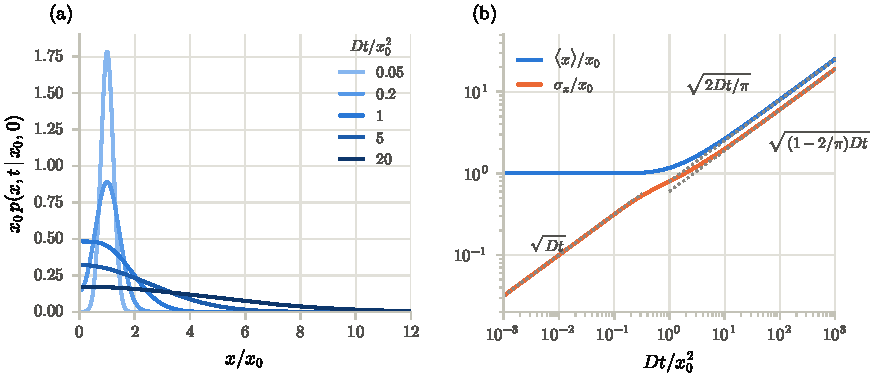
\includegraphics[width=\linewidth]{halfline_reflecting.pdf}
  \caption{Half-line, reflecting at $0$. Lengths are in units of $x_0$.
  (a)~Density snapshots. The density spreads without limit and develops zero slope at the wall.
  (b)~Mean and standard deviation, with their short- and long-time asymptotes (dotted).}
  \label{fig:hl-reflecting}
\end{figure}

% ==============================================================================
\section{Free diffusion on the half-line, absorbing at 0}
\label{sec:hl-absorbing}

\begin{keyresults}
$A=0$, $B=D$ on $(0,\infty)$, $p=0$ at $x=0$. Brownian motion killed on first reaching $0$; equivalently,
the first passage of free Brownian motion to a level a distance $x_0$ away.
\begin{align}
  P_k(x) &= \frac2\pi\sin kx,\quad Q_k(x)=\sin kx,\quad \lambda=\tfrac12Dk^2,\quad k>0
  \quad\text{(continuous; no QSD)} \\
  p(x,t\given x_0,0) &= g(x-x_0,t)-g(x+x_0,t)
  = \frac2\pi\int_0^\infty\sin kx\,\sin kx_0\,e^{-Dk^2t/2}\,\dd k \\
  S(t\given x_0) &= \operatorname{erf}\frac{x_0}{\sqrt{2Dt}}
  \;\xrightarrow{\;t\to\infty\;}\; x_0\sqrt{\frac{2}{\pi Dt}} \label{eq:HA-surv}\\
  f(t\given x_0) &= \frac{x_0}{\sqrt{2\pi Dt^3}}\,e^{-x_0^2/2Dt},\qquad
  \tilde f(s)=e^{-x_0\sqrt{2s/D}} \quad\text{(L\'evy--Smirnov)} \label{eq:HA-flux}\\
  \Pr(T<\infty) &= 1,\qquad \avg{T}=\infty,\qquad
  t_{\text{mode}}=\frac{x_0^2}{3D},\qquad t_{\text{median}}\approx2.20\,\frac{x_0^2}{D} \\
  q(x,t) &\to \frac{x}{Dt}\,e^{-x^2/2Dt}\quad\text{(Rayleigh)},\qquad \kappa(t)\to\frac{1}{2t}
\end{align}
\end{keyresults}

\paragraph{Physical picture.} A cliff (\cref{fig:walls}b): a random walker on a plateau whose edge is at $x=0$;
whoever reaches the edge falls off and is gone. Physically, a perfectly sticky or reactive surface, a detector, or
an exit. It is also the simplest random-walk neuron: the membrane potential wanders and the cell fires when it
first reaches threshold~\cite{gerstein}. Without drift the time to fire is the L\'evy--Smirnov first-passage time,
with an infinite mean.

\paragraph{From Gardiner.} The wall is \G{5.2.14}. The survival probability is Gardiner's $G(x_0,t)$
\G{5.2.140}, which obeys the backward equation \G{5.2.144} with $G(x_0,0)=1$ and $G(0,t)=0$
\G{5.2.145}--\G{5.2.146}; $\operatorname{erf}(x_0/\sqrt{2Dt})$ is that solution. The mean exit time for
``$b$ reflecting, $a$ absorbing'' \G{5.2.161} with $\psi=1$ gives $T=\frac2D\int_0^{x_0}(b-y)\,\dd y$, which
diverges as the reflecting wall $b$ moves to infinity: that is the $\avg T=\infty$ in the box.

\subsection{Images and first passage}

The absorbing wall needs $p=0$ at $x=0$, so the copy of $g$ at $-x_0$ now enters with a minus sign: the image
of \cref{sec:hl-reflecting} with the opposite sign. Integrating over $x>0$ gives $S$, and $f=-\partial_tS$ is
the L\'evy--Smirnov density \cref{eq:HA-flux}. The spectrum keeps only $\sin kx$, which vanishes at the wall as
both $P$ and $Q$ must \G{5.2.91}; the weight $2/\pi$ is the same as with the reflecting wall.

Because the line is recurrent (\cref{sec:line}), every path is eventually absorbed. But $S\sim t^{-1/2}$ goes
to zero too slowly for $\int S\,\dd t=\avg{T}$ to converge. The typical time is finite: the density $f$ peaks at $x_0^2/3D$, and half of all paths are absorbed by
$2.20\,x_0^2/D$, where $\operatorname{erf}(x_0/\sqrt{2Dt})=\tfrac12$.

The same function answers a question about free motion on the line (reflection principle). The probability
that a free path from $x_0$ has hit a level $a$ by time $t$ is
$\Pr(\min_{s\le t}x(s)\le a)=\operatorname{erfc}\bigl((x_0-a)/\sqrt{2Dt}\bigr)=1-S$.

\subsection{Conditioned on survival: no QSD}

For $Dt\gg x_0^2$, $g(x-x_0)-g(x+x_0)\simeq2g(x,t)\,xx_0/Dt$. Dividing by $S$ gives
\begin{equation}
  q(x,t)\simeq\frac{x}{Dt}\,e^{-x^2/2Dt},
\end{equation}
a Rayleigh density with scale $\sqrt{Dt}$ and mean $\sqrt{\pi Dt/2}$. It keeps spreading, so there is no
quasi-stationary state (\cref{fig:hl-absorbing}b). This is the result in \texttt{qsd-context.md} with
$D'=D/2$. The exit rate $\kappa=f/S\to1/2t$ goes to zero.
\begin{itemize}
  \item Why no QSD: the spectrum starts at $\lambda=0$ with no gap, and no $\sin kx$ is positive. The
        $k\to0$ limit of the eigenfunctions, $P_k/k\to2x/\pi$, is positive but not normalisable. The
        Rayleigh profile is that $x$ times a spreading Gaussian envelope.
  \item With a drift toward the wall a continuum of QSDs appears; that comes in Part~II.
  \item Conditioning on never being absorbed is the Doob transform with $h=x$. It adds the drift $D/x$, which
        gives the three-dimensional Bessel process. The same transform reappears in \cref{sec:absorbing}, for
        paths conditioned to leave through the far wall.
  \item A confining force freezes the Rayleigh profile into a QSD, the one a point start reaches: see the
        Ornstein--Uhlenbeck version, which also has heavier-tailed QSDs,
        \cref{sec:ou-hl-absorbing}.
\end{itemize}

\begin{figure}[tbp]
  \centering
  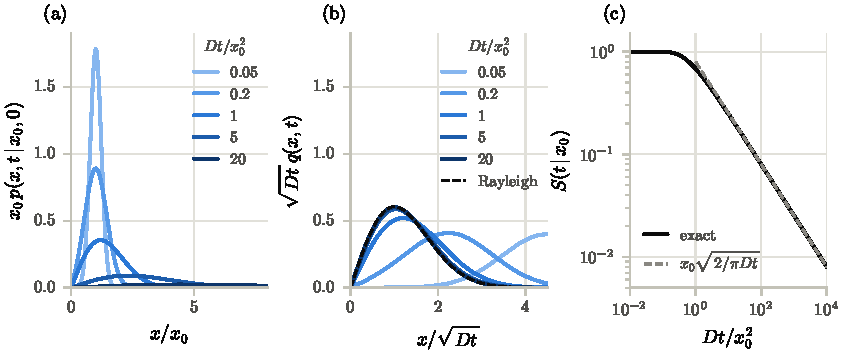
\includegraphics[width=\linewidth]{halfline_absorbing.pdf}
  \caption{Half-line, absorbing at $0$; lengths in units of $x_0$.
  (a)~Density snapshots: mass leaks out at the wall and the remainder spreads.
  (b)~The conditioned density, rescaled by the diffusion length $\sqrt{Dt}$, collapses onto the Rayleigh
  profile $u\,e^{-u^2/2}$ for $Dt\gg x_0^2$; it does not settle in $x$.
  (c)~Survival decays algebraically, $S\sim x_0\sqrt{2/\pi Dt}$.}
  \label{fig:hl-absorbing}
\end{figure}

% ==============================================================================
\section{Free diffusion, reflecting walls}
\label{sec:reflecting}

\begin{keyresults}
$A=0$, $B=D$ on $(0,L)$, $\partial_xp=0$ at $x=0,L$. SDE $\dd x=\sqrt D\,\dd W$, reflected at the walls.
Gardiner \Gs{5.2.6b} does the case $L=D=1$.
\begin{align}
  \lambda_n &= \frac{n^2\pi^2D}{2L^2},\quad n=0,1,2,\dots \quad
  Q_0=1,\quad Q_n(x)=\sqrt2\cos\frac{n\pi x}{L},\quad P_n=\frac{Q_n}L \label{eq:R-spectrum}\\
  p(x,t\given x_0,0) &= \frac1L + \frac2L\sum_{n\ge1}\cos\frac{n\pi x}{L}\cos\frac{n\pi x_0}{L}\,e^{-\lambda_nt} \notag\\
  &= \sum_{m\in\mathbb Z}\bigl[g(x-x_0+2mL,t)+g(x+x_0+2mL,t)\bigr] \label{eq:R-prop}\\
  p_s &= 1/L, \qquad \text{relaxation time } 1/\lambda_1 = \frac{2L^2}{\pi^2D}\approx 0.203\,\frac{L^2}{D}\\
  C(\tau) &\equiv \avg{x(\tau)x(0)}_s-\avg{x}_s^2 = \frac{8L^2}{\pi^4}\nodd\frac{e^{-\lambda_n|\tau|}}{n^4},
  \qquad C(0)=\frac{L^2}{12}
\end{align}
with free kernel $g(y,t)=(2\pi Dt)^{-1/2}e^{-y^2/2Dt}$.
\end{keyresults}

\paragraph{Physical picture.} A particle in a closed box or channel of length $L$, with hard walls at both
ends: a bead in a sealed microfluidic chamber, or a protein in a cell compartment. $\mathcal U=0$ inside. The
relaxation time $2L^2/\pi^2D$ is the mixing time of the box.

\paragraph{From Gardiner.} \Gs{5.2.6b} does exactly this case for $L=D=1$. It gives the cosine series
\G{5.2.102}--\G{5.2.107}, the stationary autocorrelation \G{5.2.109}--\G{5.2.110}, and the identity \G{5.2.114}.
He does not name $P_n$ and $Q_n$ there, but \G{5.2.107} is \G{5.2.88} with $P_n=Q_n=\sqrt2\cos n\pi x$, since
$p_s=1$.
To restore $L$ and $D$, replace $n\pi x$ by $n\pi x/L$ and $\lambda_n=\tfrac12n^2\pi^2$ \G{5.2.106} by
$n^2\pi^2D/2L^2$. The stationary density $1/L$ is \cref{eq:ps} with $A=0$. The moments, $\tau_c$ and the image
form are additions.

\subsection{Spectrum and propagator}

Start from the half-line of \cref{sec:hl-reflecting}, whose modes are $\cos kx$ for every $k\ge0$. The second
wall at $L$ needs $Q'(L)=0$ as well, which allows only $k_n=n\pi/L$: \cref{eq:R-spectrum}. The continuum
becomes a ladder, and a gap $\lambda_1=\pi^2D/2L^2$ opens (\cref{sec:gap}). Now $p_s=1/L$ is normalisable, and
Gardiner's normalisation $\int p_sQ_n^2=1$ gives $Q_0=1$, $Q_n=\sqrt2\cos(n\pi x/L)$ and $P_n=p_sQ_n=Q_n/L$, which
is the mode sum in \cref{eq:R-prop}.

The image form says the same thing in position space. Mirror the source at $0$, as in
\cref{sec:hl-reflecting}; that pair must also be mirrored at $L$, which gives another pair, which must be
mirrored at $0$, and so on. The result is a lattice of image pairs with period $2L$. Mode sum and image sum
are the same function by Poisson summation. The image sum converges fast for $Dt\ll L^2$ (only the source and the
nearest images matter), the mode sum for $Dt\gtrsim L^2$. They agree to machine precision (\cref{app:checks}).

\subsection{Relaxation and moments}

Every mode but $n=0$ decays, so $p\to1/L$. The slowest rate is $\lambda_1$, unless the start is symmetric:
for $x_0=L/2$ all odd modes vanish, since $\cos(n\pi/2)=0$, and the relaxation goes at $\lambda_2=4\lambda_1$.

Using $\int_0^Lx\cos(n\pi x/L)\,\dd x=[(-1)^n-1]L^2/n^2\pi^2$ and
$\int_0^Lx^2\cos(n\pi x/L)\,\dd x=2(-1)^nL^3/n^2\pi^2$,
\begin{align}
  \avg{x(t)} &= \frac L2-\frac{4L}{\pi^2}\nodd\frac{1}{n^2}\cos\frac{n\pi x_0}{L}\,e^{-\lambda_nt}, \\
  \avg{x^2(t)} &= \frac{L^2}{3}+\frac{4L^2}{\pi^2}\sum_{n\ge1}\frac{(-1)^n}{n^2}\cos\frac{n\pi x_0}{L}\,e^{-\lambda_nt}.
\end{align}
At $t=0$ these reduce to $x_0$ and $x_0^2$, by the Fourier series of $\theta$ and $\theta^2$ on $(0,\pi)$.
For $Dt\ll\min(x_0,L-x_0)^2$ the walls are not felt and $\sigma_x^2\approx Dt$; for $Dt\gg L^2$,
$\avg x\to L/2$ and $\sigma_x^2\to L^2/12$ (\cref{fig:reflecting}b).

\subsection{Stationary autocorrelation}

Only odd modes have $\int x\,P_n\neq0$, which gives $C(\tau)$ in the box \G{5.2.110}. The identity
$\nodd n^{-4}=\pi^4/96$ \G{5.2.114} gives $C(0)=L^2/12$, the variance of the uniform distribution.
\begin{itemize}
  \item The slowest mode carries a fraction $96/\pi^4\approx0.986$ of the variance, so $C(\tau)$ is a
        single exponential to within 1.5\,\% (\cref{fig:reflecting}c).
  \item The integrated correlation time is exact: with $\nodd n^{-6}=\pi^6/960$,
        \begin{equation}
          \tau_c=\int_0^\infty\frac{C(\tau)}{C(0)}\,\dd\tau=\frac{L^2}{5D}
          \qquad\text{vs.}\qquad \frac1{\lambda_1}=\frac{2L^2}{\pi^2D}\approx\frac{L^2}{4.93\,D}.
        \end{equation}
  \item The initial slope is $C'(0^+)=-D/2$, since $C(0)-C(\tau)=\tfrac12\avg{[x(\tau)-x(0)]^2}\approx
        \tfrac12D\tau$. The one-mode approximation gives $-4D/\pi^2\approx-0.41\,D$ instead; the missing part
        sits in the fast modes.
\end{itemize}

\begin{figure}[tbp]
  \centering
  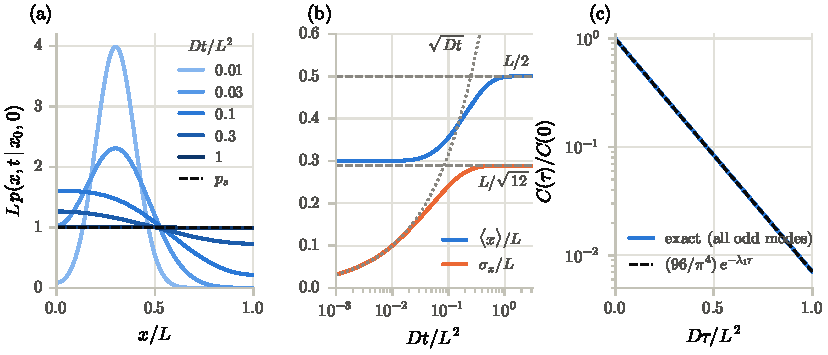
\includegraphics[width=\linewidth]{reflecting.pdf}
  \caption{Reflecting walls, $x_0=0.3L$.
  (a)~Density snapshots relaxing to $p_s=1/L$.
  (b)~Mean and standard deviation. At short times $\sigma_x\approx\sqrt{Dt}$ (dotted); both saturate on the
  time scale $1/\lambda_1\approx0.2\,L^2/D$. Here $x_0$ happens to lie close to $L/\sqrt{12}$, so $\avg x$
  starts near the lower dashed line.
  (c)~Normalised stationary autocorrelation. The exact series and the single slowest mode are
  indistinguishable on this scale.}
  \label{fig:reflecting}
\end{figure}

% ==============================================================================
\section{Free diffusion, absorbing walls}
\label{sec:absorbing}

\begin{keyresults}
$A=0$, $B=D$ on $(0,L)$, $p=0$ at $x=0,L$. SDE $\dd x=\sqrt D\,\dd W$, killed at the walls.
Gardiner \Gs{5.2.6a} does the propagator for $L=D=1$; first passage is \Gs{5.2.7}--\Gs{5.2.8}.
\begin{align}
  \lambda_n &= \frac{n^2\pi^2D}{2L^2},\quad n=1,2,\dots \quad Q_n(x)=\sqrt2\sin\frac{n\pi x}{L},\quad P_n=\frac{Q_n}L \\
  p(x,t\given x_0,0) &= \frac2L\sum_{n\ge1}\sin\frac{n\pi x}{L}\sin\frac{n\pi x_0}{L}\,e^{-\lambda_nt} \notag\\
  &= \sum_{m\in\mathbb Z}\bigl[g(x-x_0+2mL,t)-g(x+x_0+2mL,t)\bigr] \label{eq:A-prop}\\
  S(t\given x_0) &= \frac4\pi\nodd\frac1n\sin\frac{n\pi x_0}{L}\,e^{-\lambda_nt}
  \;\xrightarrow{\;t\to\infty\;}\; \frac4\pi\sin\frac{\pi x_0}{L}\,e^{-\lambda_1t} \label{eq:A-surv}\\
  \pi_0 &= 1-\frac{x_0}{L},\qquad \pi_L=\frac{x_0}{L} \\
  T(x_0) &= \frac{x_0(L-x_0)}{D},\qquad
  \operatorname{Var}T = \frac{x_0(L-x_0)\bigl[x_0^2+(L-x_0)^2\bigr]}{3D^2} \\
  T_0(x_0) &= \frac{x_0(2L-x_0)}{3D},\qquad T_L(x_0)=\frac{L^2-x_0^2}{3D} \\
  q_\infty(x) &= \frac{\pi}{2L}\sin\frac{\pi x}{L},\qquad \kappa(t)\to\lambda_1=\frac{\pi^2D}{2L^2}\approx4.93\,\frac{D}{L^2}
\end{align}
\end{keyresults}

\paragraph{Physical picture.} A plateau between two cliffs, or a pore open at both ends from which a molecule
escapes through either mouth. The classic discrete version is the gambler's ruin: a fortune of $x_0$ against
$L-x_0$, changed by fair bets until one player is broke, with $\pi_L=x_0/L$.

\paragraph{From Gardiner.} \Gs{5.2.6a} gives the sine series \G{5.2.92}--\G{5.2.100} for $L=D=1$, with the
absorbing-wall convention for $P_\lambda,Q_\lambda$ of \G{5.2.91}: \G{5.2.100} is \G{5.2.88} with
$P_n=Q_n=\sqrt2\sin n\pi x$. With $\psi=1$ the first-passage machinery
of \Gs{5.2.7}--\Gs{5.2.8} integrates in elementary functions:
\begin{itemize}
  \item $T$ from \G{5.2.154}, or directly from \G{5.2.158};
  \item $T_2$ from the hierarchy \G{5.2.156} with $n=2$;
  \item $\pi_0,\pi_L$ from \G{5.2.186}--\G{5.2.190};
  \item $T_0,T_L$ from \G{5.2.183} with \G{5.2.185}.
\end{itemize}
The QSD is not in the book; it is the $n=1$ term of \G{5.2.100}, normalised.

\subsection{Spectrum and propagator}

This is \cref{sec:hl-absorbing} with a second absorbing wall, exactly as \cref{sec:reflecting} was
\cref{sec:hl-reflecting} with a second mirror. The half-line's $\sin kx$ must also vanish at $L$, so
$k_n=n\pi/L$. The nonzero spectrum is identical to the reflecting interval, but $n=0$ is missing, so nothing
survives. Gardiner's convention takes $p_s=1/L$ from the reflecting problem \G{5.2.91}, so the normalisation is
the same as there: $Q_n=\sqrt2\sin(n\pi x/L)$, $P_n=Q_n/L$, both zero at the walls. In the image sum each image
is the negative mirror image of the one before, which makes $p$ vanish at both walls.

Letting $L\to\infty$ recovers \cref{sec:hl-absorbing}, and the interval results show how the half-line's
peculiarities arise:
\begin{itemize}
  \item $\pi_L=x_0/L\to0$: the path reaches $0$ with probability one (recurrence);
  \item $T=x_0(L-x_0)/D\to\infty$: it takes infinitely long on average;
  \item $\lambda_1=\pi^2D/2L^2\to0$: the gap closes and the decay of $S$ becomes algebraic.
\end{itemize}

\begin{figure}[tbp]
  \centering
  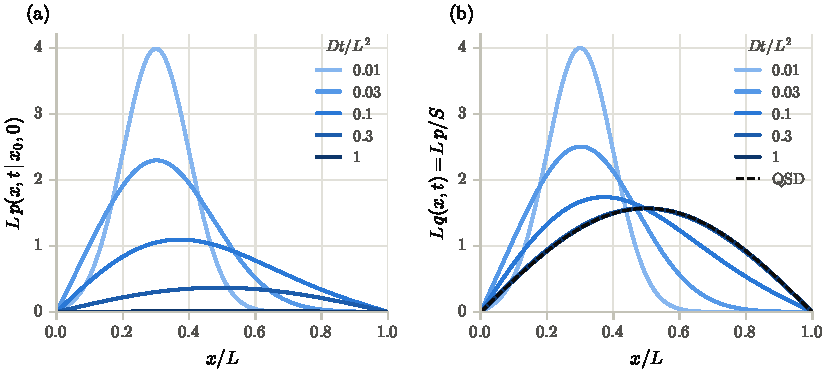
\includegraphics[width=\linewidth]{absorbing_density.pdf}
  \caption{Absorbing walls, $x_0=0.3L$.
  (a)~$p(x,t\given x_0,0)$ loses mass through both walls.
  (b)~The density conditioned on survival, $q=p/S$, converges to the QSD $\frac{\pi}{2L}\sin\frac{\pi x}{L}$
  (dashed) by $Dt/L^2\approx0.3$.}
  \label{fig:absorbing-density}
\end{figure}

\subsection{Survival, exit-time density, exit through each wall}

Integrating the mode sum gives \cref{eq:A-surv}. Only odd $n$ contribute, and $S(0)=1$ because
$\sum_{n\,\mathrm{odd}}\sin(n\theta)/n=\pi/4$ on $(0,\pi)$. The exit-time density and the outward fluxes
through each wall, $j_0=\tfrac12D\,\partial_xp|_{x=0}$ and $j_L=-\tfrac12D\,\partial_xp|_{x=L}$, are
\begin{align}
  f(t\given x_0) &= -\partial_tS = \frac{2\pi D}{L^2}\nodd n\sin\frac{n\pi x_0}{L}\,e^{-\lambda_nt}, \\
  j_0(t\given x_0) &= \frac{\pi D}{L^2}\sum_{n\ge1} n\sin\frac{n\pi x_0}{L}\,e^{-\lambda_nt}
  = \sum_{m\in\mathbb Z}\frac{x_0+2mL}{\sqrt{2\pi Dt^3}}\exp\!\Bigl[-\frac{(x_0+2mL)^2}{2Dt}\Bigr],
  \label{eq:A-flux}
\end{align}
and $j_L(t\given x_0)=j_0(t\given L-x_0)$. The image form is a sum of half-line L\'evy--Smirnov densities
\cref{eq:HA-flux}, one per image; the $m=0$ term is \cref{sec:hl-absorbing} itself. It dominates while
$Dt\ll x_0^2$. In that regime the walls act
independently:
$1-S\approx\operatorname{erfc}\bigl(x_0/\sqrt{2Dt}\bigr)+\operatorname{erfc}\bigl((L-x_0)/\sqrt{2Dt}\bigr)$.

\paragraph{Laplace transforms.} With $k=\sqrt{2s/D}$, solving $\tfrac12D\tilde f''=s\tilde f$ in $x_0$ with
the appropriate wall values gives
\begin{equation}
  \tilde j_0(s)=\frac{\sinh k(L-x_0)}{\sinh kL},\qquad
  \tilde j_L(s)=\frac{\sinh kx_0}{\sinh kL},\qquad
  \tilde f(s)=\frac{\cosh k(x_0-L/2)}{\cosh(kL/2)} .
\end{equation}
Expanding in $s$ gives all the moments below, e.g.\ $\tilde f=1-s\,x_0(L-x_0)/D+O(s^2)$.

\begin{figure}[tbp]
  \centering
  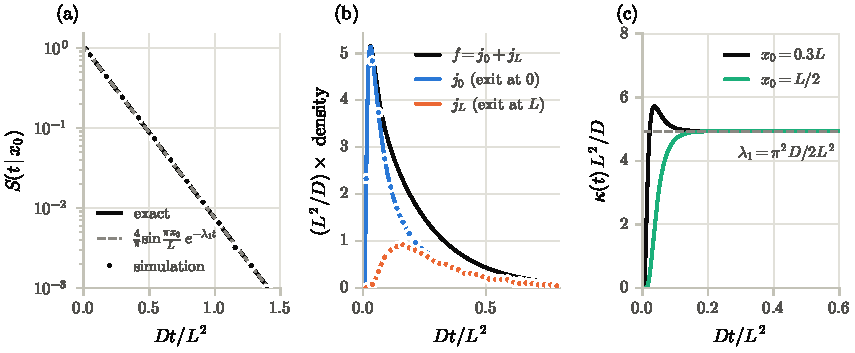
\includegraphics[width=\linewidth]{absorbing_exit.pdf}
  \caption{Absorbing walls, exit statistics.
  (a)~Survival from $x_0=0.3L$ against the one-mode asymptote, with simulation points.
  (b)~Exit-time density $f$ and its split into exits through each wall, \cref{eq:A-flux}; dots are
  histograms of $5\times10^4$ simulated paths.
  (c)~Exit rate $\kappa=f/S$ from two starting points. Both settle at $\lambda_1$; from $x_0=0.3L$ it
  overshoots first.}
  \label{fig:absorbing-exit}
\end{figure}

\subsection{Splitting probabilities and exit times}

With $A=0$, $\psi=1$ in \G{5.2.157}, and the backward equations of \cref{sec:fpt-toolkit} integrate directly.
\begin{itemize}
  \item $\pi_L=x_0/L$ \G{5.2.190}: the gambler's-ruin result.
  \item $T(x_0)=x_0(L-x_0)/D$, which follows from $\tfrac12DT''=-1$. Its maximum is $L^2/4D$ at the centre;
        averaged over a uniform start it is $L^2/6D$.
  \item The second moment is $T_2=x_0(L-x_0)(L^2+Lx_0-x_0^2)/3D^2$, which gives $\operatorname{Var}T$ in the
        box. At the centre $\sigma_T=L^2/\sqrt{24}\,D$, so the coefficient of variation is
        $\sqrt{2/3}\approx0.82$: the exit time is not sharply defined.
  \item Conditional exit times. Paths that start near $0$ but leave through $L$ take
        $T_L\to L^2/3D$. Conditioning on exit at $L$ is the Doob transform with $h=\pi_L=x/L$; it adds the
        drift $B\,\partial_x\ln h=D/x$, which makes the conditioned process a three-dimensional Bessel process.
\end{itemize}

\begin{figure}[tbp]
  \centering
  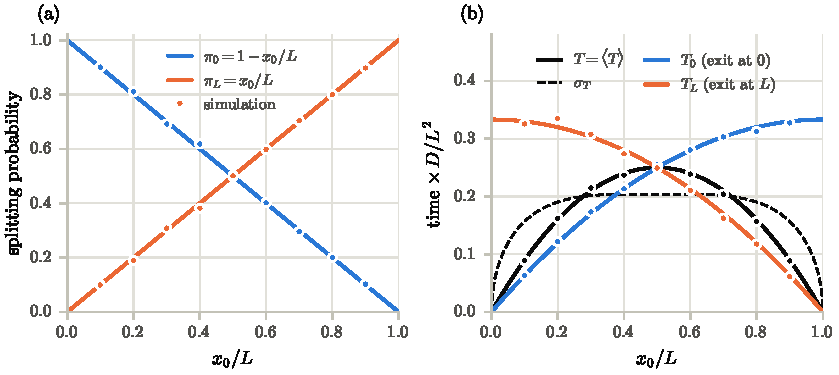
\includegraphics[width=\linewidth]{absorbing_exit_times.pdf}
  \caption{Absorbing walls, dependence on the starting point.
  (a)~Splitting probabilities.
  (b)~Mean exit time $T$, its standard deviation $\sigma_T$, and the conditional means $T_0$, $T_L$. Dots
  are simulation means over 4000 paths per starting point.
  At the centre $\sigma_T=0.204\,L^2/D$, close to but not equal to $1/\lambda_1=0.203\,L^2/D$.}
  \label{fig:absorbing-exit-times}
\end{figure}

\subsection{Long times: quasi-stationary distribution}

For $t\gg1/(\lambda_2-\lambda_1)$ only $n=1$ survives:
$p\simeq\frac2L\sin\frac{\pi x_0}{L}\sin\frac{\pi x}{L}e^{-\lambda_1t}$. Therefore
\begin{itemize}
  \item $q=p/S\to q_\infty=\frac{\pi}{2L}\sin\frac{\pi x}{L}$, independent of $x_0$ (\cref{fig:absorbing-density}b).
  \item $\kappa(t)\to\lambda_1$. The approach goes at $\lambda_2-\lambda_1=3\lambda_1$, or at
        $\lambda_3-\lambda_1=8\lambda_1$ for $x_0=L/2$, where the even modes vanish by symmetry
        (\cref{fig:absorbing-exit}c).
  \item Starting in $q_\infty$, $S=e^{-\lambda_1t}$ exactly and $T$ is exponential with mean
        $1/\lambda_1=2L^2/\pi^2D$. Consistency check:
        $\int_0^Lq_\infty(x_0)\,T(x_0)\,\dd x_0=1/\lambda_1$, using
        $\int_0^Lx(L-x)\sin(\pi x/L)\,\dd x=4L^3/\pi^3$.
  \item The QSD is the ground state $P_1$, normalised as a density: $q_\infty=P_1/\int P_1$.
  \item Conditioning on survival \emph{forever} (the $Q$-process) gives a different stationary density,
        $P_1Q_1=\frac2L\sin^2\frac{\pi x}{L}$, already normalised by \G{5.2.79}. The process is
        $\dd x=\frac{\pi D}{L}\cot\frac{\pi x}{L}\,\dd t+\sqrt D\,\dd W$.
\end{itemize}

\paragraph{Overshoot in $\kappa$.} For $x_0=0.3L$, $\kappa(t)$ rises above $\lambda_1$ before settling. Early on,
$q$ sits nearer the wall at $0$ than $q_\infty$ does, so it leaks faster than the QSD. From $x_0=L/2$ the
density is far from both walls and $\kappa$ rises monotonically.

\subsection{Reflecting vs.\ absorbing}

\begin{itemize}
  \item The spectra are the same, $\{n^2\pi^2D/2L^2\}$, except that only the reflecting case includes $n=0$.
  \item The reflecting decay rate $\lambda_1$ toward $p_s$ equals the absorbing decay rate of $S$. The
        absorbing $q$ relaxes faster, at $3\lambda_1$.
  \item The eigenfunctions are $\cos$ vs.\ $\sin$, and the image signs are $+$ vs.\ $-$.
\end{itemize}

% ==============================================================================
\section{Free diffusion, reflecting at 0, absorbing at \texorpdfstring{$L$}{L}}
\label{sec:mixed}

\begin{keyresults}
$A=0$, $B=D$ on $(0,L)$, $\partial_xp=0$ at $x=0$, $p=0$ at $x=L$. SDE $\dd x=\sqrt D\,\dd W$, reflected
at $0$ and killed at $L$. Every exit is through $L$. Gardiner gives $T$ in \G{5.2.160}. With $k_n=(2n+1)\pi/2L$:
\begin{align}
  \lambda_n &= \frac{(2n+1)^2\pi^2D}{8L^2},\quad n=0,1,2,\dots \qquad
  Q_n(x)=\sqrt2\cos k_nx,\quad P_n=\frac{Q_n}L \\
  p(x,t\given x_0,0) &= \frac2L\sum_{n\ge0}\cos k_nx\,\cos k_nx_0\,e^{-\lambda_nt} \notag\\
  &= \sum_{m\in\mathbb Z}(-1)^m\bigl[g(x-x_0+2mL,t)+g(x+x_0+2mL,t)\bigr] \label{eq:M-prop}\\
  S(t\given x_0) &= \frac4\pi\sum_{n\ge0}\frac{(-1)^n}{2n+1}\cos k_nx_0\,e^{-\lambda_nt}
  \;\xrightarrow{\;t\to\infty\;}\; \frac4\pi\cos\frac{\pi x_0}{2L}\,e^{-\lambda_0t} \\
  f(t\given x_0) &= \sum_{m\in\mathbb Z}(-1)^m\,\frac{(2m+1)L-x_0}{\sqrt{2\pi Dt^3}}
  \exp\!\Bigl[-\frac{((2m+1)L-x_0)^2}{2Dt}\Bigr],\qquad
  \tilde f(s)=\frac{\cosh kx_0}{\cosh kL} \label{eq:M-flux}\\
  T(x_0) &= \frac{L^2-x_0^2}{D},\qquad \operatorname{Var}T=\frac{2(L^4-x_0^4)}{3D^2} \\
  q_\infty(x) &= \frac{\pi}{2L}\cos\frac{\pi x}{2L},\qquad
  \kappa(t)\to\lambda_0=\frac{\pi^2D}{8L^2}\approx1.23\,\frac{D}{L^2}
\end{align}
\end{keyresults}

\paragraph{Physical picture.} A dead-end tube: a hard wall at one end and an open end, a cliff, at the other.
Examples are a molecule leaving a closed-ended pore, or a protein leaving a dendritic spine through its neck. The
mean time to get out from the closed end, $L^2/D$, is four times that from the middle of a tube of the same
length open at both ends.

\paragraph{From Gardiner.} This is the case ``$a$ reflecting, $b$ absorbing'' of \Gs{5.2.7b}. Its backward
boundary conditions \G{5.2.159} lead to the closed form \G{5.2.160}, which with $\psi=1$ is
$T=\frac2D\int_{x_0}^L y\,\dd y$. The $Q_n$ obey the reflecting backward condition \G{5.2.69} at $0$
and the absorbing one \G{5.2.67} at $L$, so they are cosines with $\cos k_nL=0$; $P_n=p_sQ_n$ with $p_s=1/L$ from
the reflecting interval \G{5.2.91}. Everything else follows by unfolding into \cref{sec:absorbing}.

\subsection{Unfolding into an interval of length \texorpdfstring{$2L$}{2L}}

A reflecting wall is a mirror, as in \cref{sec:hl-reflecting}. Extend $p$ evenly to $(-L,L)$: the extension solves the free equation with
$p=0$ at $\pm L$, started from $\tfrac12[\delta(x-x_0)+\delta(x+x_0)]$. So this problem is the absorbing
interval of \cref{sec:absorbing} with $L\to2L$, restricted to initial data symmetric about the centre.
\begin{itemize}
  \item The spectrum of the length-$2L$ interval is $n'^2\pi^2D/8L^2$. The symmetric modes are those with
        odd $n'=2n+1$; they are the $\cos k_nx$ above. The antisymmetric (even $n'$) modes are never excited.
  \item The ground state is $4\times$ slower than with both walls absorbing:
        $\lambda_0=\pi^2D/8L^2$ vs.\ $\pi^2D/2L^2$. The gap is $\lambda_1-\lambda_0=8\lambda_0$.
  \item In the image sum \cref{eq:M-prop} each image pair repeats with period $2L$ and alternating sign, so the
        full pattern has period $4L$.
  \item Every result for the starting point $x_0=0$ here equals the result for the centre of an absorbing
        interval of length $2L$. For example $T(0)=L^2/D=(2L)^2/4D$.
\end{itemize}
The other orientation, absorbing at $0$ and reflecting at $L$, follows from $x\to L-x$.

\subsection{Survival and exit time}

With $\int_0^L\cos k_nx\,\dd x=(-1)^n/k_n$, the mode sum gives $S$; $S(0)=1$ because
$\sum_{n\ge0}(-1)^n\cos((2n+1)\theta)/(2n+1)=\pi/4$ for $|\theta|<\pi/2$. The image form of $f$ in
\cref{eq:M-flux} is the absorbing-interval flux \cref{eq:A-flux} on $(-L,L)$, summed over both walls. Its
$m=0$ term is the L\'evy--Smirnov density for the distance $L-x_0$.

The backward equation $\tfrac12D\tilde f''=s\tilde f$ with $\tilde f'(0)=0$ and $\tilde f(L)=1$ gives
$\tilde f=\cosh kx_0/\cosh kL$, with $k=\sqrt{2s/D}$. Its expansion gives the moments.
\begin{itemize}
  \item $T=(L^2-x_0^2)/D$. This is \G{5.2.160} with $\psi=1$:
        $T=2\int_{x_0}^L\dd y\int_0^y\dd z/D$. The largest value is $L^2/D$, at the reflecting wall.
  \item $T_2=(5L^4-6L^2x_0^2+x_0^4)/3D^2$, so $\operatorname{Var}T=2(L^4-x_0^4)/3D^2$. At $x_0=0$ the
        coefficient of variation is $\sqrt{2/3}$, the same as at the centre of the absorbing interval, as the
        unfolding requires.
  \item Starting from the QSD, $T$ is exponential with mean $1/\lambda_0=8L^2/\pi^2D\approx0.81\,L^2/D$.
        Check: $\int_0^Lq_\infty(x_0)\,T(x_0)\,\dd x_0=1/\lambda_0$.
\end{itemize}

\subsection{Long times}

The ground state dominates once $t\gg1/8\lambda_0$:
\begin{itemize}
  \item $q\to q_\infty=\frac{\pi}{2L}\cos\frac{\pi x}{2L}$. The QSD is flat at the reflecting wall and
        vanishes linearly at the absorbing one.
  \item $\kappa\to\lambda_0$.
  \item The $Q$-process has stationary density $P_0Q_0=\frac2L\cos^2\frac{\pi x}{2L}$, from the SDE
        $\dd x=-\frac{\pi D}{2L}\tan\frac{\pi x}{2L}\,\dd t+\sqrt D\,\dd W$.
\end{itemize}

\begin{figure}[tbp]
  \centering
  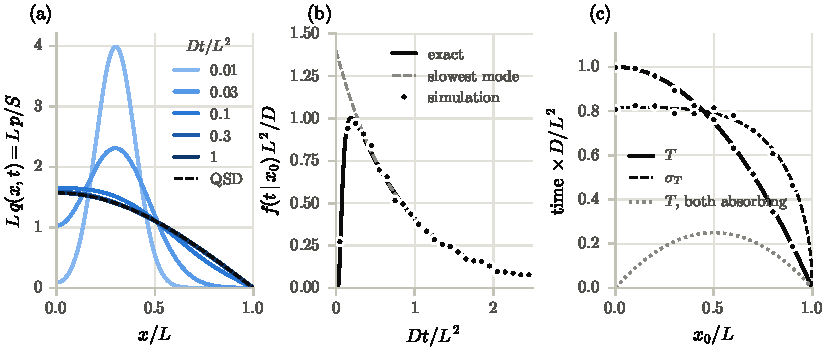
\includegraphics[width=\linewidth]{mixed.pdf}
  \caption{Reflecting at $0$, absorbing at $L$.
  (a)~From $x_0=0.3L$, $q=p/S$ converges to the QSD $\frac{\pi}{2L}\cos\frac{\pi x}{2L}$ (dashed).
  (b)~The exit-time density \cref{eq:M-flux} from $x_0=0.3L$, against the slowest mode alone and a histogram
  of $2\times10^4$ simulated paths.
  (c)~Mean and standard deviation of the exit time; dots are means over 4000 paths. The dotted curve is
  $T$ with both walls absorbing, for comparison.}
  \label{fig:mixed}
\end{figure}

% ==============================================================================
\section{Free diffusion on the circle}
\label{sec:circle}

\begin{keyresults}
$A=0$, $B=D$ on the circle $S^1=\mathbb R/L\mathbb Z$ (\cref{sec:circle-toolkit}): no walls and no special
point. With $R=L/2\pi$ and angle $\theta=x/R$ this is the rotational diffusion of a planar rotor. With
$q_m=2\pi m/L$:
\begin{align}
  p(x,t\given x_0,0) &= \sum_{n\in\mathbb Z}g(x-x_0+nL,t)
  =\frac1L+\frac2L\sum_{m\ge1}\cos q_m(x-x_0)\,e^{-\lambda_mt} \label{eq:C-prop}\\
  \lambda_m &= \tfrac12Dq_m^2=\frac{2\pi^2m^2D}{L^2},\quad P_m=\frac{e^{iq_mx}}L,\quad Q_m=e^{-iq_mx},\quad
  m\in\mathbb Z \\
  p_s &= \frac1L,\qquad J_s=0,\qquad \text{relaxation time }\frac1{\lambda_1}=\frac{L^2}{2\pi^2D}\approx0.051\,\frac{L^2}{D} \\
  \avg{e^{iq_m[x(t)-x(0)]}} &= e^{-\lambda_m|t|},\qquad\text{e.g. }\avg{\cos\Delta\theta(t)}=e^{-Dt/2R^2} \\
  \Delta\tilde x &\ \text{Gaussian, mean }0,\ \text{variance }Dt\ \text{exactly}:\qquad v_{\rm w}=0,\quad D_{\text{eff}}=D \\
  T(d) &= \frac{d(L-d)}{D},\qquad \Pr(\text{arrive moving in the }{+x}\text{ direction})=\frac dL,\qquad T_{\rm w}=\frac{L^2}D
\end{align}
Here $T(d)$ is the mean time to reach a target from a distance $d$ above it (measured in the $+x$ direction),
and $T_{\rm w}$ the mean time to the first full winding.
\end{keyresults}

\paragraph{Physical picture.} A bead on a circular track with no force along it (\cref{fig:walls}c): a colloid in
a ring-shaped optical trap of uniform intensity, or the orientation of a rod rotating in a plane. For the rotor,
$x/R$ is the angle, $D/2R^2$ the rotational diffusion coefficient, and $\avg{\cos\Delta\theta}=e^{-Dt/2R^2}$ Debye's
orientational relaxation in two dimensions.

\paragraph{From Gardiner.} The book's periodic results are \G{5.2.17}--\G{5.2.19} and the stationary solution
\G{5.2.41}--\G{5.2.47}. With $A=0$, $\psi=1$, so \G{5.2.46} gives $J=0$ and \G{5.2.47} a uniform $p_s$. The
propagator comes from the Wiener process of \Gs{3.8.1} in two ways:
\begin{itemize}
  \item summing the Gaussian \G{3.8.7} over the lifts \cref{eq:cover} gives the image form;
  \item for a variable that lives on a circle, only the values $s=q_m$ of the characteristic function
        \G{3.8.6} are defined, since $e^{isx}$ is a function on the circle only for those $s$. They are exactly
        the Fourier coefficients of $p$, and $\phi(q_m,t)=e^{iq_mx_0-Dq_m^2t/2}$ gives the mode sum.
\end{itemize}
\Gs{5.2.5} is written for reflecting and absorbing walls; with periodic $Q$ its boundary terms are simply
absent. With $p_s=1/L$, the real form of each doublet is $Q_m=\sqrt2\cos q_mx$, $\sqrt2\sin q_mx$ with
$P_m=p_sQ_m=Q_m/L$, exactly as on the reflecting interval; the complex pair in the box is the same doublet.

\subsection{From the line}

\Cref{eq:cover} applied to the Gaussian of \cref{sec:line} gives the image form of \cref{eq:C-prop}: the free
Gaussian, wrapped around the circle (\cref{fig:circle}b). Poisson summation turns it into the mode sum. As on the
intervals, the image sum converges fast for $Dt\ll L^2$ and the mode sum for $Dt\gtrsim L^2$, and they agree to
$10^{-15}$. Compare the reflecting interval \cref{eq:R-prop}, where the images come in mirror pairs with period
$2L$. Here there is one image per lattice point, with period $L$ and no mirrors.

\subsection{Folding: the circle is two intervals}

$A=0$ is odd under every reflection, so the folding of \cref{sec:circle-toolkit} works about any point. Fold
about the start $x_0$, which fixes $x_0$ and its antipode $x_0+L/2$:
\begin{itemize}
  \item The even sector is the reflecting interval of length $L/2$ (\cref{sec:reflecting}), with levels
        $n^2\pi^2D/2(L/2)^2=2\pi^2n^2D/L^2$, $n\ge0$. The odd sector is the absorbing interval of length $L/2$
        (\cref{sec:absorbing}), with the same nonzero levels. Together they give each $\lambda_m$ twice: the
        doublet $\cos q_m(x-x_0)$, $\sin q_m(x-x_0)$ (\cref{fig:circle}c).
  \item A point start is even about itself, so only the even sector is excited. The propagator on the circle
        is exactly half the reflecting propagator on $(0,L/2)$ started at a wall:
        $p(x,t\given x_0,0)=\tfrac12p_{\rm R}(|x-x_0|,t\given0,0)$.
  \item The gap $2\pi^2D/L^2$ is four times that of the reflecting interval of length $L$: on the circle the
        farthest point is only $L/2$ away.
\end{itemize}

\subsection{Observables and relaxation}

\begin{itemize}
  \item $\avg{x(t)}$ has no meaning here: $x$ jumps at the cut, so the answer depends on where the cut is.
        The Fourier modes are good observables, and each is a single eigenfunction:
        $\avg{e^{iq_mx(t)}}=e^{iq_mx_0-\lambda_mt}$ exactly, with no admixture of other rates. For the rotor,
        $\lambda_1=D/2R^2$ and this is Debye's $\avg{\cos\Delta\theta}=e^{-Dt/2R^2}$.
  \item The density relaxes to $1/L$ at $\lambda_1$, in a time $\approx0.05\,L^2/D$ (\cref{fig:circle}a).
\end{itemize}

\subsection{Winding and first passage}

\begin{itemize}
  \item The lift is exactly free motion on the line: $\Delta\tilde x$ is Gaussian with variance $Dt$ at all
        times, so $v_{\rm w}=0$ and $D_{\rm eff}=D$. The circle changes where the particle is, not how far it has
        gone.
  \item The first full winding is the absorbing interval $(x_0-L,x_0+L)$ on the cover, started at its centre:
        $T_{\rm w}=(2L)^2/4D=L^2/D$ by \cref{sec:absorbing}. Then $L^2/T_{\rm w}=D=D_{\rm eff}$, as the renewal
        argument of \cref{sec:circle-toolkit} requires.
  \item First passage to a target: cut there, and the circle becomes the absorbing interval of length $L$ of
        \cref{sec:absorbing}, with $x_0\to d$. The mean time is longest, $L^2/4D$, from the antipode. The
        particle arrives by the shorter way round with probability $\max(d,L-d)/L$.
\end{itemize}

\begin{figure}[tbp]
  \centering
  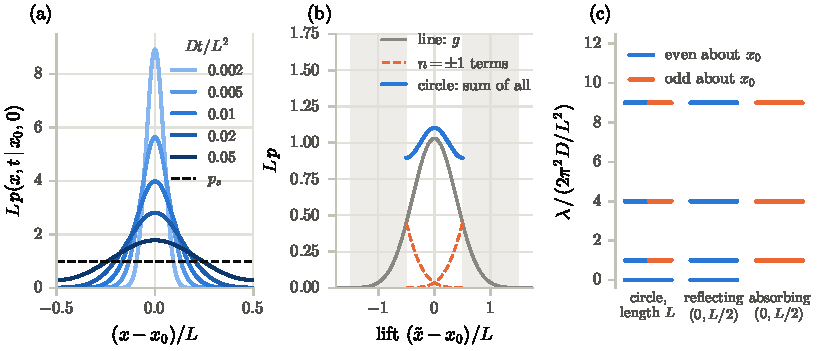
\includegraphics[width=\linewidth]{circle.pdf}
  \caption{Free diffusion on the circle, centred on the starting point (the only distinguished point).
  (a)~Density snapshots relaxing to $1/L$ by $Dt/L^2\approx0.05$.
  (b)~The universal cover at $Dt/L^2=0.15$: the free Gaussian on the line (grey), its translates by $\pm L$
  folded into one period (dashed), and their sum, the density on the circle (blue). Shading marks the
  neighbouring copies of the circle.
  (c)~Spectrum in units of $2\pi^2D/L^2$. Each nonzero level of the circle is a doublet: one level from the
  reflecting interval of length $L/2$ (even about $x_0$) and one from the absorbing one (odd).}
  \label{fig:circle}
\end{figure}

% ==============================================================================
\section{Summary of free diffusion}
\label{sec:free-summary}

\begin{table}[h]
\centering
\small
\renewcommand{\arraystretch}{1.3}
\begin{tabular}{@{}l l l l@{}}
\toprule
Walls & Slowest rate & Long-time law & Mean exit time $T(x_0)$ \\
\midrule
reflecting $0$, $L$   & $\pi^2D/2L^2$ & $p\to1/L$                               & --- \\
absorbing $0$, $L$    & $\pi^2D/2L^2$ & $S\propto e^{-\pi^2Dt/2L^2}$            & $x_0(L-x_0)/D$ \\
refl.\ $0$, abs.\ $L$ & $\pi^2D/8L^2$ & $S\propto e^{-\pi^2Dt/8L^2}$            & $(L^2-x_0^2)/D$ \\
reflecting $0$ only   & $0$ (no gap)  & $p\simeq\sqrt{2/\pi Dt}\,e^{-x^2/2Dt}$  & --- \\
absorbing $0$ only    & $0$ (no gap)  & $S\simeq x_0\sqrt{2/\pi Dt}$           & $\infty$ \\
none                  & $0$ (no gap)  & $p=g(x-x_0,t)$                          & --- \\
circle                & $2\pi^2D/L^2$ (doublet) & $p\to1/L$                     & to a target: $d(L-d)/D$ \\
\bottomrule
\end{tabular}
\caption{Free diffusion, $\partial_tp=\tfrac12D\,\partial_x^2p$, in every geometry.}
\label{tab:free-summary}
\end{table}

\begin{itemize}
  \item A bounded domain has a discrete spectrum with a gap, so relaxation and decay are exponential. An
        unbounded domain has a continuous spectrum reaching $\lambda=0$, so everything is algebraic in $t$.
  \item With absorption on a bounded domain the conditioned density goes to a QSD, the positive ground state.
        Without a bound it spreads (Rayleigh) and there is no QSD.
  \item The slowest rate depends on the walls, not just the size. A reflecting wall is a mirror and doubles
        the effective length, so the rate drops by $4$ (\cref{fig:free-summary}c).
  \item The two reflecting cases differ only near the far wall at $L$ (\cref{fig:free-summary}a). The
        absorbing ones differ everywhere, because each absorbing wall pins $p$ to $0$
        (\cref{fig:free-summary}b).
  \item The circle has no walls. Folded about the start it is a reflecting interval of half its length, so it
        relaxes four times faster than the reflecting interval of the same length. Its winding is exactly
        free motion on the line.
\end{itemize}

\begin{figure}[tbp]
  \centering
  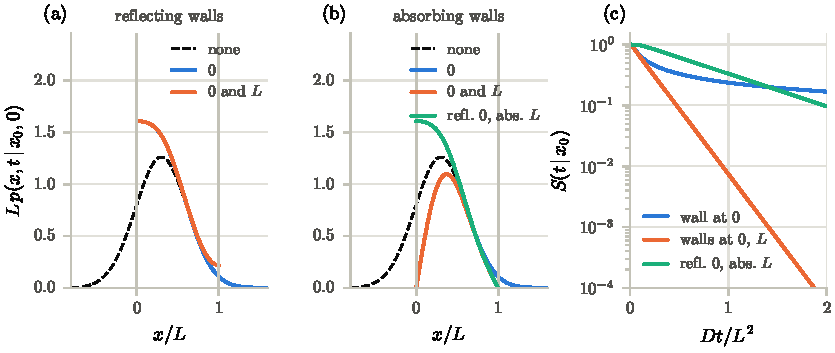
\includegraphics[width=\linewidth]{free_summary.pdf}
  \caption{Free diffusion in every geometry, all from $x_0=0.3L$.
  (a,b)~Densities at $Dt/L^2=0.1$; grey vertical lines mark $x=0$ and $x=L$, and the dashed curve is the
  free Gaussian. A wall ``at $0$'' alone is the half-line.
  (c)~Survival for the three absorbing geometries: $e^{-\pi^2Dt/2L^2}$, $e^{-\pi^2Dt/8L^2}$, and
  $t^{-1/2}$ for the half-line, which overtakes the mixed interval near $Dt/L^2\approx1.4$.}
  \label{fig:free-summary}
\end{figure}

% ==============================================================================
\part{Constant drift: \texorpdfstring{$A=v$, $B=D$}{A=v, B=D}}
\label{part:drift}

\section{Constant drift: reduction to free diffusion}
\label{sec:drift-gauge}

The equation is $\partial_tp=-v\,\partial_xp+\tfrac12D\,\partial_x^2p$, from $\dd x=v\,\dd t+\sqrt D\,\dd W$;
$v>0$ drifts toward $+x$. It is the overdamped motion in the linear potential $U=-vx$
($A=-U'$). In every drift figure blue means $v<0$ (toward $x=0$), red $v>0$, and grey $v=0$.

\paragraph{Physical picture.} A constant force $F$, so $\mathcal U=-Fx$ and $v=F/\gamma$
(\cref{sec:physical}): gravity minus buoyancy on a colloid (sedimentation), an electric field on a charged particle
(electrophoresis), or a uniform flow carrying a solute (advection). The drift length $\ell=D/|v|=2k_BT/|F|$ is the
distance over which the force does work $2k_BT$, so the P\'eclet number $L/\ell$ compares the work done by the
force across the system with the thermal energy.

\paragraph{From Gardiner.} The stationary solution \cref{eq:ps} \G{5.2.39} with $A=v$, $B=D$ gives
$p_s\propto e^{2vx/D}$ at once. Everything else in Part~II comes from Part~I through the transformation
below, which is not in the book. It is the one-dimensional case of removing a constant drift from the heat
equation, equivalently the Girsanov factor.

\paragraph{Drift scales.} Unlike free diffusion, the dynamics now has its own length and time,
\begin{equation}
  \ell\equiv\frac{D}{|v|},\qquad \tau\equiv\frac{\ell^2}{D}=\frac{\ell}{|v|}=\frac{D}{v^2}:
  \label{eq:drift-scales}
\end{equation}
over a length $\ell$ drift and diffusion are comparable, and $\tau$ is the time to cross it either way.
\begin{itemize}
  \item Every other length enters only through a P\'eclet number, $L/\ell=|v|L/D$ for the interval or
        $x_0/\ell=|v|x_0/D$ for the start. These describe the geometry and the initial condition, not the dynamics.
  \item Results at fixed $v\neq0$ below are written in $\ell$ and $\tau$. Figures that sweep $v$ through $0$
        keep $L$ or $x_0$ as the unit, because $\ell\to\infty$ as $v\to0$.
  \item Factor of two: because $B=D$ means a diffusion constant $D/2$, the barometric profile decays over
        $\ell/2$. Defining $\ell$ as $D/|v|$ rather than $D/2|v|$ keeps the gauge constant below simple:
        $\alpha=\pm1/\ell$.
\end{itemize}

\paragraph{Gauge transformation.} With $\alpha\equiv v/D=\operatorname{sgn}(v)/\ell$,
\begin{equation}
  p(x,t)=\exp\Bigl[\alpha(x-x_0)-\frac{t}{2\tau}\Bigr]\,u(x,t),\qquad \partial_tu=\tfrac12D\,\partial_x^2u .
  \label{eq:gauge}
\end{equation}
Substituting, the terms in $\partial_xu$ cancel because $\alpha=v/D$, and the terms in $u$ cancel because the
exponent decays at $1/2\tau=v^2/2D$. The prefactor equals 1 at $x=x_0$, $t=0$, so $u$ also starts as
$\delta(x-x_0)$. This is the symmetrisation of \cref{sec:operator}: $e^{\alpha x}\propto\sqrt{p_s}$, the
potential \cref{eq:schrodinger} is the constant $V=1/2\tau$, and $u$ solves the free problem once that constant
is taken out.

\paragraph{Walls.} Since $J=vp-\tfrac12D\,\partial_xp=\tfrac12De^{(\cdots)}\bigl[\alpha u-\partial_xu\bigr]$:
\begin{itemize}
  \item absorbing, $p=0$ $\iff$ $u=0$, so absorbing problems are free problems times the prefactor;
  \item reflecting, $J=0$ $\iff$ $\partial_xu=\alpha u=\pm u/\ell$, a Robin condition, so reflecting problems
        change character.
\end{itemize}

\paragraph{Consequences.}
\begin{itemize}
  \item The spectrum is shifted: $\lambda=1/2\tau+\tfrac12Dk^2$, where $k$ comes from the $u$-problem.
        Drift alone sets a decay rate $1/2\tau=v^2/2D$, independent of its sign.
  \item Gardiner's eigenfunctions are $P_n\propto e^{\alpha x}u_n$ (forward) and $Q_n\propto e^{-\alpha x}u_n$
        (backward), with $u_n$ orthogonal in plain $L^2$. Since $\sqrt{p_s}\propto e^{\alpha x}$, this is
        \cref{eq:PQ-psi} with $\psi_n=u_n/\sqrt{N_n}$, and his normalisation is
        \begin{equation}
          P_n=\sqrt{\frac{p_s}{N_n}}\,u_n,\qquad Q_n=\frac{u_n}{\sqrt{N_np_s}},\qquad N_n=\int u_n^2\,\dd x .
          \label{eq:drift-PQ}
        \end{equation}
        Here $p_s$ is the zero-current solution $\propto e^{2\alpha x}$: normalised where it can be (on an
        interval, and on the half-line for $v<0$), any multiple of $e^{2\alpha x}$ otherwise, and that of the
        reflecting problem when a wall absorbs \G{5.2.91}. Hence
        \begin{equation}
          p(x,t\given x_0,0)=e^{\alpha(x-x_0)}\sum_n\frac{u_n(x)\,u_n(x_0)}{N_n}\,e^{-\lambda_nt}.
          \label{eq:gauge-modes}
        \end{equation}
        The operator is not self-adjoint in $L^2$. The prefactor $e^{\alpha(x-x_0)}$, as large as $e^{L/\ell}$,
        means the slowest mode can take a transit time $L/|v|=(L/\ell)\,\tau$ to dominate.
  \item Through an absorbing wall at $x=w$ the exit flux is
        $j_w(t)=e^{\alpha(w-x_0)-t/2\tau}\,j_w^{\,\text{free}}(t)$.
  \item For the first-passage formulas of \cref{sec:fpt-toolkit}, $\psi=e^{2\alpha x}$.
\end{itemize}

% ==============================================================================
\section{Constant drift on the whole line}
\label{sec:drift-line}

\begin{keyresults}
$A=v$, $B=D$ on $(-\infty,\infty)$: Brownian motion with drift \Gs{3.8.3}.
\begin{align}
  p(x,t\given x_0,0) &= g(x-x_0-vt,t),\qquad \avg x=x_0+vt,\qquad \operatorname{Var}x=Dt \\
  P_k &= \frac{e^{(\alpha+ik)x}}{2\pi},\quad Q_k=e^{-(\alpha+ik)x},\quad \lambda=\frac1{2\tau}+\tfrac12Dk^2\quad
  \text{(in the gauge)} \\
  \avg{e^{ikx(t)}} &= e^{ik(x_0+vt)-Dk^2t/2} \\
  f_a(t) &= \frac{a-x_0}{\sqrt{2\pi Dt^3}}\,e^{-(a-x_0-vt)^2/2Dt}\qquad\text{(first passage to }a>x_0) \\
  \Pr(\text{reach }a) &= \begin{cases}1&v\ge0\\e^{-2(a-x_0)/\ell}&v<0\end{cases}
\end{align}
The spreading $\sqrt{Dt}$ equals the displacement $|v|t$ at $t=\tau$, where both are $\ell$: diffusion
dominates for $t\ll\tau$, drift for $t\gg\tau$.
\end{keyresults}

\paragraph{Physical picture.} A colloid sedimenting far above the floor of its container, an ion drifting in a
field, or a pollutant carried down a river: the cloud moves at $v$ and spreads as $\sqrt{Dt}$.

\paragraph{From Gardiner.} The book meets this Gaussian in \Gs{3.8.3}, as the small-step approximation of the
Poisson process, a one-sided random walk: \G{3.8.58} is the density with mean $vt$ and variance $Dt$, and
\G{3.8.59} its Fokker--Planck equation. (Gardiner stresses that this is an expansion, not a limit.) Here it is \cref{sec:line} pushed through \cref{eq:gauge}.

\begin{itemize}
  \item A Galilean shift $x\to x-vt$ removes the drift on the line, but not in the presence of a wall,
        which does not move. That is why every bounded example in this part depends on $v$.
  \item The gauge \cref{eq:gauge} is the statement that $g(x-x_0-vt)=e^{\alpha(x-x_0)-t/2\tau}g(x-x_0)$. In
        path language it is the Girsanov factor, which depends only on the endpoints and $t$. That is why
        absorbing problems, which constrain only endpoints, transform so simply.
  \item \textbf{Two sets of eigenfunctions.} The gauge gives the $P_k$, $Q_k$ of the box, with real
        $\lambda=1/2\tau+\tfrac12Dk^2$: the spectrum in $L^2(1/p_s)$, $p_s\propto e^{2\alpha x}$. But the plain
        Fourier modes $P_k=e^{ikx}/2\pi$, $Q_k=e^{-ikx}$ are eigenfunctions too, bounded, with complex
        $\lambda=\tfrac12Dk^2+ivk$; the characteristic function in the box is their statement. Both sums
        \G{5.2.88} give $g(x-x_0-vt)$. Which is ``the'' spectrum depends on the space (\cref{sec:operator}); on the
        circle only the Fourier modes survive (\cref{sec:drift-circle}).
  \item First passage to a level will be \cref{sec:drift-hl-absorbing} with $x_0\to a-x_0$ and $v\to-v$.
        Drift toward the level makes $\avg T=(a-x_0)/v$ finite; drift away makes reaching it uncertain.
\end{itemize}

% ==============================================================================
\section{Constant drift on the half-line, reflecting at 0}
\label{sec:drift-hl-reflecting}

\begin{keyresults}
$A=v$, $B=D$ on $(0,\infty)$, $J=0$ at $x=0$ (Smoluchowski's sedimentation problem). With
$\alpha=v/D=\pm1/\ell$ and $\tau=D/v^2$:
\begin{align}
  p(x,t\given x_0,0) &= g(x-x_0-vt,t)+e^{-2\alpha x_0}g(x+x_0-vt,t)
  -\alpha\,e^{2\alpha x}\operatorname{erfc}\frac{x+x_0+vt}{\sqrt{2Dt}} \label{eq:DHR-prop}\\
  P_k &= \sqrt{\frac{p_s}{N_k}}\,u_k,\quad Q_k=\frac{u_k}{\sqrt{N_kp_s}},\quad \lambda=\frac1{2\tau}+\tfrac12Dk^2,
  \quad k>0 \\
  u_k &= \cos kx+\frac\alpha k\sin kx,\qquad N_k=\frac\pi2\Bigl(1+\frac{\alpha^2}{k^2}\Bigr),\qquad
  p_s\propto e^{2\alpha x} \\
  v<0:\quad p_s(x) &= \frac2\ell\,e^{-2x/\ell},\quad \avg x_s=\frac\ell2;\quad P_0=p_s,\ Q_0=1;\quad
  \text{spectrum } \{0\}\cup\Bigl[\frac1{2\tau},\infty\Bigr) \\
  v>0:\quad p &\simeq g(x-x_0-vt,t),\quad \avg{x}\simeq vt=\ell\,\frac t\tau\quad\text{(no stationary state)}
\end{align}
\end{keyresults}

\paragraph{In drift units.} With $\xi=x/\ell$, $s=t/\tau$, $\xi_0=x_0/\ell$ and
$G_s(y)=e^{-y^2/2s}/\sqrt{2\pi s}$, the case $v<0$ reads
\begin{equation}
  \ell\,p=G_s(\xi-\xi_0+s)+e^{2\xi_0}G_s(\xi+\xi_0+s)+e^{-2\xi}\operatorname{erfc}\frac{\xi+\xi_0-s}{\sqrt{2s}} .
\end{equation}
There is one parameter, $\xi_0$, and at long times $\ell p\to2e^{-2\xi}$ whatever it is.

\paragraph{Physical picture.} For $v<0$: colloids settling onto the floor of a container. The barometric profile
$e^{-2x/\ell}=e^{-|F|x/k_BT}$ is the sedimentation equilibrium from which Perrin measured Avogadro's
number~\cite{perrin}; for gas molecules in gravity it is the barometric formula of the atmosphere. For $v>0$ the
force points away from the floor, as for buoyant droplets released at the bottom of a tall column: they rise and
never return.

\paragraph{From Gardiner.} The wall is the zero-current condition \G{5.2.13}. The stationary solution
\cref{eq:ps} with $\psi=e^{2vx/D}$ gives $p_s$, which on $(0,\infty)$ is normalisable only for $v<0$ (compare
the infinite-range discussion of \Gs{5.2.2c}). The time dependence needs the Robin image below, which is not
in the book.

\subsection{The Robin image}

Pushed through \cref{eq:gauge}, the mirror of \cref{sec:hl-reflecting} becomes the Robin condition
$u'=\alpha u$, and a single image no longer suffices. The combination
$w=u'-\alpha u$ obeys the free equation with $w=0$ at the wall, so it is a Dirichlet problem, solved by one
image pair. Then integrating $u'-\alpha u=w$ inward from $x=\infty$ gives
\begin{equation}
  u=g(x-x_0)+g(x+x_0)-2\alpha\int_x^\infty e^{-\alpha(\xi-x)}g(\xi+x_0,t)\,\dd\xi ,
\end{equation}
a point image plus a line of images beyond $-x_0$ with weight $e^{\alpha\xi}$. Completing the square in the
integral gives the erfc term, and \cref{eq:gauge} turns the point image into $e^{-2\alpha x_0}g(x+x_0-vt)$. The
script checks normalisation, $J(0)=0$, and the PDE residual of \cref{eq:DHR-prop}.

\paragraph{The same in eigenfunctions.} The Robin modes of \cref{sec:drift-reflecting}, with $k$ now continuous,
are the $u_k$ of the box; $\int_0^\infty u_ku_{k'}\,\dd x=N_k\,\delta(k-k')$ fixes $N_k$, and \cref{eq:drift-PQ}
gives $P_k$ and $Q_k$, with $p_s\propto e^{2\alpha x}$ (for $v>0$ any multiple). For $v<0$ the Robin condition also
has the bound state $u=e^{\alpha x}$, which decays and gives $P_0=p_s$, $Q_0=1$; for $v>0$ it grows and is not an
eigenfunction. Then $\int_0^\infty P_k(x)Q_k(x_0)e^{-\lambda t}\,\dd k$, plus $P_0(x)Q_0(x_0)=p_s(x)$ if $v<0$, is
\cref{eq:DHR-prop} (checked to $10^{-15}$).

\subsection{Long times}

\begin{itemize}
  \item $v<0$ (drift into the wall): the erfc tends to $2$ and the Gaussians leave, so
        $p\to(2/\ell)e^{-2x/\ell}$: sedimentation equilibrium (\cref{fig:drift-hl-reflecting}a). The spectrum
        is the isolated $\lambda=0$ plus a continuum from $1/2\tau$, so the gap is $1/2\tau$ although the
        domain is unbounded.
  \item $v>0$: the packet moves off at speed $v$, and the wall only matters while it is within about
        $\sqrt{Dt}$ of it.
  \item $v=0$ is \cref{sec:hl-reflecting}: $\avg x\sim\sqrt{2Dt/\pi}$. The three regimes are visible in
        \cref{fig:drift-hl-reflecting}b. At $vx_0/D=-0.5$ the start sits at $\avg x_s=\ell/2$, and the mean
        dips before returning.
\end{itemize}

\begin{figure}[tbp]
  \centering
  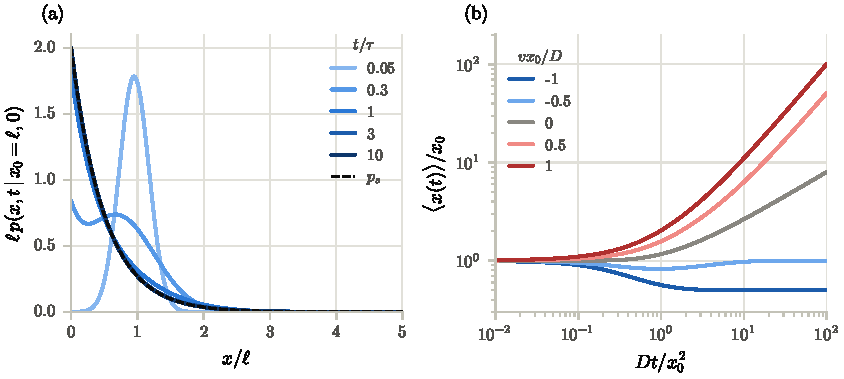
\includegraphics[width=\linewidth]{drift_halfline_reflecting.pdf}
  \caption{Constant drift on the half-line, reflecting at $0$.
  (a)~Relaxation to the barometric profile for $v<0$, in drift units $\ell=D/|v|$, $\tau=D/v^2$, from
  $x_0=\ell$.
  (b)~Mean position for several drifts, in units of $x_0$ because the sweep passes through $v=0$:
  saturation at $\ell/2$ for $v<0$, $\sqrt t$ for $v=0$, $vt$ for $v>0$.}
  \label{fig:drift-hl-reflecting}
\end{figure}

% ==============================================================================
\section{Constant drift on the half-line, absorbing at 0}
\label{sec:drift-hl-absorbing}

\begin{keyresults}
$A=v$, $B=D$ on $(0,\infty)$, $p=0$ at $x=0$. With $\alpha=v/D=\pm1/\ell$ and $\tau=D/v^2$:
\begin{align}
  p(x,t\given x_0,0) &= g(x-x_0-vt,t)-e^{-2\alpha x_0}g(x+x_0-vt,t) \\
  P_k &= \sqrt{\tfrac{2p_s}{\pi}}\,\sin kx,\quad Q_k=\sqrt{\tfrac{2}{\pi p_s}}\,\sin kx,\quad
  \lambda=\frac1{2\tau}+\tfrac12Dk^2\quad(p_s\propto e^{2\alpha x}) \\
  S(t\given x_0) &= \tfrac12\Bigl[\operatorname{erfc}\Bigl(-\frac{x_0+vt}{\sqrt{2Dt}}\Bigr)
  -e^{-2\alpha x_0}\operatorname{erfc}\frac{x_0-vt}{\sqrt{2Dt}}\Bigr] \\
  f(t\given x_0) &= \frac{x_0}{\sqrt{2\pi Dt^3}}\,e^{-(x_0+vt)^2/2Dt},\qquad
  \tilde f(s)=e^{-\alpha x_0-x_0\sqrt{\alpha^2+2s/D}}\quad\text{(inverse Gaussian)} \\
  \Pr(T<\infty) &= \begin{cases}1 & v\le0\\ e^{-2x_0/\ell} & v>0\end{cases},\qquad
  v<0:\ \avg T=\frac{x_0}{\ell}\,\tau,\ \ \operatorname{Var}T=\frac{x_0}{\ell}\,\tau^2 \\
  v<0:\ \ \phi_\lambda &\propto e^{r_+x}-e^{r_-x},\quad r_\pm=-\frac{1\mp\sqrt{1-2\lambda\tau}}{\ell},
  \quad 0<\lambda\le\frac1{2\tau}\quad\text{(a continuum of QSDs)} \\
  q(x,t) &\to \frac{x}{\ell^2}\,e^{-x/\ell}\ \text{(point start)},\qquad
  S\simeq\sqrt{\frac2\pi}\,\frac{x_0}{\ell}\,e^{x_0/\ell}\Bigl(\frac t\tau\Bigr)^{-3/2}e^{-t/2\tau},\qquad
  \kappa\simeq\frac1{2\tau}+\frac3{2t} \\
  q(x,t) &\to \phi_\lambda\ \text{with }r_+=-\beta,\ \ \lambda=\beta|v|-\tfrac12D\beta^2
  \quad\text{if }p(x,0)\sim e^{-\beta x},\ \beta<1/\ell
\end{align}
\end{keyresults}

This is the problem of \texttt{qsd-context.md} \S3--4 (there with drift $-\mu$ and $D'=D/2$) and of the
preset \texttt{halfline} in \texttt{sde-explorer}.

\paragraph{Physical picture.} A walker on a slope that ends in a cliff. For $v<0$ the slope runs toward the
edge: colloids sedimenting onto a sticky floor, or the Gerstein--Mandelbrot neuron, whose membrane potential drifts
toward threshold~\cite{gerstein}; its interspike interval is then the inverse-Gaussian first-passage time of this
section. For $v>0$ the slope runs away from the edge, and a walker that starts a few $\ell$ from it almost surely
never falls.

\paragraph{From Gardiner.} With the far wall at infinity, everything in \Gs{5.2.7}--\Gs{5.2.8} applies with
$\psi=e^{2vx/D}$.
\begin{itemize}
  \item The probability of ever reaching $0$ is $\pi_0$ from the corrected \G{5.2.189} with $b\to\infty$:
        $\pi_0=\int_{x_0}^\infty\dd y/\psi\big/\int_0^\infty\dd y/\psi$. This is $e^{-2x_0/\ell}$ for $v>0$, and
        $1$ for $v\le0$, where both integrals diverge.
  \item For $v<0$, $\avg T=x_0/|v|$ solves \G{5.2.154} with $T(0)=0$ and $T$ bounded at infinity.
\end{itemize}

\subsection{Propagator and first passage}

Absorbing, so the gauge maps the image pair of \cref{sec:hl-absorbing} straight over. The exit-time density
is the L\'evy--Smirnov density times $e^{-\alpha x_0-t/2\tau}$: the inverse Gaussian.
\begin{itemize}
  \item $v<0$: absorption is certain, with $\avg T=x_0/|v|$ (ballistic) and a tail cut off at $t\sim\tau$
        (\cref{fig:drift-hl-absorbing}b). The relative spread is $\sigma_T/\avg T=\sqrt{\ell/x_0}$, so the
        exit time is sharp only for a start many drift lengths away.
  \item $v>0$: the path escapes to $\infty$ with probability $1-e^{-2x_0/\ell}$, and $f$ integrates to
        $e^{-2x_0/\ell}$. A start a few drift lengths out almost always escapes.
  \item $v=0$: the $t^{-3/2}$ tail and $\avg T=\infty$ of \cref{sec:hl-absorbing}.
\end{itemize}

\subsection{A continuum of QSDs}

For $v<0$, $\tfrac12D\phi''-v\phi'+\lambda\phi=0$ with $\phi(0)=0$ has roots $r_\pm$ that are both
negative for $0<\lambda\le1/2\tau$, so $\phi_\lambda$ is positive and integrable: every such $\lambda$ gives a
QSD (\cref{fig:drift-hl-absorbing}c). For $\lambda>1/2\tau$ the roots are complex and $\phi$ oscillates. In
the symmetrised variable, $\phi=e^{\alpha x}\psi$, the $L^2$ spectrum is the continuum $[1/2\tau,\infty)$.
The QSDs below the edge have $\psi$ growing like $e^{(r_+-\alpha)x}$: not in $L^2$, but $\phi$ is in $L^1$. In
Gardiner's terms $\phi_\lambda$ is a forward eigenfunction $P_\lambda$ whose partner $Q_\lambda=\phi_\lambda/p_s$
grows like $e^{(r_++2/\ell)x}$, so $\int P_\lambda Q_\lambda$ \G{5.2.79} diverges and $\lambda$ has no place in
\G{5.2.88}. A
second wall at $L$ removes all but one; compare \cref{sec:drift-absorbing}, where
$\lambda_1=1/2\tau+\pi^2D/2L^2\to1/2\tau$ as $L\to\infty$.

\subsection{Which QSD is reached}

The tail of the initial density decides (\cref{sec:spectrum-states}, \cref{fig:attraction}a).
\begin{itemize}
  \item \textbf{Point start.} The gauge turns the problem into the free absorbing half-line, whose conditioned
        density spreads as the Rayleigh profile $(x/Dt)e^{-x^2/2Dt}$ (\cref{sec:hl-absorbing}). Near the wall
        that is $\propto x$, and the gauge factor $e^{-x/\ell}$ freezes it into the edge QSD
        $xe^{-x/\ell}/\ell^2$: a Gamma(2) density with mean $2\ell$, independent of $x_0$. The approach is
        algebraic, because the edge of a continuum has no gap: $\kappa\simeq1/2\tau+3/2t$
        (\cref{fig:drift-hl-absorbing}a). The drift length sets the QSD completely; $x_0$ only sets how long the
        transient lasts.
  \item \textbf{Exponential start}, $p(x,0)=\beta e^{-\beta x}$. In the gauge the initial condition is
        $w_0=e^{x/\ell}p(x,0)=\beta e^{\gamma x}$ with $\gamma=1/\ell-\beta$.
        \begin{itemize}
          \item If $\gamma>0$, $w_0$ grows, and the free evolution of a growing exponential does not spread:
                $u\simeq2\beta e^{\gamma^2Dt/2}\sinh\gamma x$ once $\gamma^2Dt\gg1$. Back through the gauge,
                $p\propto e^{-(1/2\tau-D\gamma^2/2)t}\bigl(e^{-\beta x}-e^{-(2/\ell-\beta)x}\bigr)$. That is
                exactly the QSD $\phi_\lambda$ with $r_+=-\beta$, and
                $\lambda=1/2\tau-\tfrac12D\gamma^2=\beta|v|-\tfrac12D\beta^2$. It is approached exponentially
                fast.
          \item If $\gamma\le0$, $w_0$ does not grow, and the start behaves like a point start: it reaches the
                edge QSD, algebraically.
        \end{itemize}
        Both cases are closed-form, since the free evolution of $e^{\gamma y}$ is a pair of Gaussian integrals;
        the script checks them.
  \item \textbf{General starts.} Mart\'inez, Picco and San Mart\'in~\cite{martinez} showed that an initial
        density with a definite exponential tail rate $\beta$ goes to the QSD this rule picks. That is the one
        with the same tail if $\beta<1/\ell$, and the edge otherwise, including tails lighter than every
        exponential. A tail heavier than every exponential gives no limit at all: the survivors are particles
        still drifting in from far out, and the conditioned density follows them outward.
  \item \textbf{Why the threshold is $1/\ell$.} A particle starting near $y$ arrives after about $y/|v|$, so a
        tail $e^{-\beta y}$ supplies survivors at the rate $\beta|v|$; diffusion lowers this by
        $\tfrac12D\beta^2$. The far supply wins when it is slower than the bulk's $1/2\tau$, which is exactly
        when $\beta<1/\ell$ (\cref{fig:attraction}c).
\end{itemize}

\begin{figure}[tbp]
  \centering
  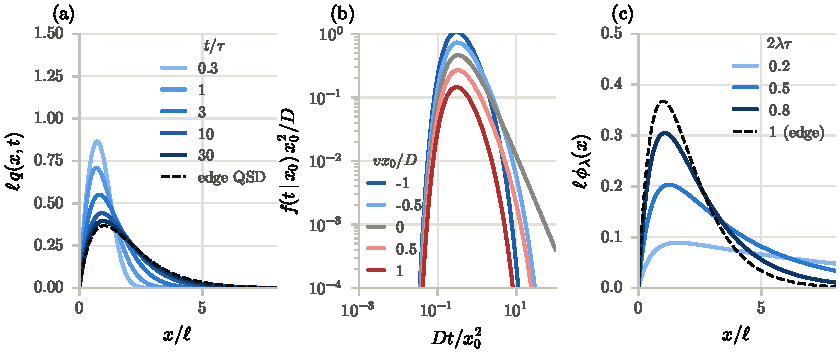
\includegraphics[width=\linewidth]{drift_halfline_absorbing.pdf}
  \caption{Constant drift on the half-line, absorbing at $0$.
  (a)~Conditioned density for $v<0$ in drift units $\ell=D/|v|$, $\tau=D/v^2$, from $x_0=\ell$, creeping
  toward the edge QSD $xe^{-x/\ell}/\ell^2$.
  (b)~Exit-time densities, in units of $x_0$ because the sweep passes through $v=0$. For $v>0$ the area is
  $e^{-2vx_0/D}<1$.
  (c)~The QSD family, in drift units: smaller $\lambda$ means a heavier tail.}
  \label{fig:drift-hl-absorbing}
\end{figure}

% ==============================================================================
\section{Constant drift, reflecting walls}
\label{sec:drift-reflecting}

\begin{keyresults}
$A=v$, $B=D$ on $(0,L)$, $J=0$ at both walls. With $\alpha=v/D=\pm1/\ell$ and $\tau=D/v^2$
(\cref{eq:drift-scales}):
\begin{align}
  p_s(x) &= \frac{2\alpha\,e^{2\alpha x}}{e^{2\alpha L}-1},\qquad
  \avg x_s=\frac{L}{1-e^{-2\alpha L}}-\frac1{2\alpha} \\
  \lambda_0 &= 0,\qquad \lambda_n=\frac1{2\tau}+\frac{n^2\pi^2D}{2L^2},\quad n\ge1 \\
  \phi_n(x) &= \cos k_nx+\frac{\alpha}{k_n}\sin k_nx,\qquad k_n=\frac{n\pi}{L},\qquad
  N_n=\int_0^L\phi_n^2\,\dd x=\frac L2\Bigl(1+\frac{\alpha^2}{k_n^2}\Bigr) \\
  P_0 &= p_s,\quad Q_0=1;\qquad P_n=\sqrt{\frac{p_s}{N_n}}\,\phi_n,\quad Q_n=\frac{\phi_n}{\sqrt{N_np_s}},\quad n\ge1 \\
  p(x,t\given x_0,0) &= p_s(x)+\frac2L\,e^{\alpha(x-x_0)}\sum_{n\ge1}
  \frac{\phi_n(x)\,\phi_n(x_0)}{1+\alpha^2/k_n^2}\,e^{-\lambda_nt} \label{eq:DR-prop}
\end{align}
\end{keyresults}

\paragraph{Physical picture.} Sedimentation in a closed column of height $L$: the barometric profile of
\cref{sec:drift-hl-reflecting}, cut off by a ceiling. An analytical ultracentrifuge reaches the same kind of
sedimentation equilibrium, with the centrifugal force in place of gravity, roughly constant across a thin cell.

\paragraph{From Gardiner.} $p_s$ is \cref{eq:ps}. The eigenfunctions are Gardiner's $P_\lambda=p_sQ_\lambda$
(\G{5.2.71}, \G{5.2.73}--\G{5.2.74}), with the reflecting backward condition \G{5.2.69}, $Q'=0$, at both walls. In the gauge
$Q\propto e^{-\alpha x}u$, so $Q'=0$ is $u'=\alpha u$; forward, $J(P_n)=0$ is the same condition. The normalisation
\G{5.2.80} is \cref{eq:drift-PQ}, and the expansion \G{5.2.84}--\G{5.2.88} then gives \cref{eq:DR-prop}.

\subsection{Spectrum}

This is the Robin wall of \cref{sec:drift-hl-reflecting}, now at both ends, just as \cref{sec:reflecting} put
the mirror of \cref{sec:hl-reflecting} at both ends. The solution regular at $x=0$ is
$\phi=\cos kx+(\alpha/k)\sin kx$; the condition at $L$ reduces to $(k+\alpha^2/k)\sin kL=0$, so
$k_n=n\pi/L$ exactly as without drift. The extra solution with imaginary $k=\pm i\alpha$ is $u=e^{\alpha x}$,
which gives $p_s\propto e^{2\alpha x}$ with $\lambda=0$. Using $\int_0^L\phi_n^2=\tfrac L2(1+\alpha^2/k_n^2)$ in
\cref{eq:gauge-modes} gives \cref{eq:DR-prop}; at $v=0$ it is \cref{eq:R-prop}.

\subsection{Stationary state and relaxation}

\begin{itemize}
  \item $p_s\propto e^{-2U/D}$ with $U=-vx$: a barometric (sedimentation) profile, piled against the wall the
        drift points to, with decay length $\ell/2$ (\cref{fig:drift-reflecting}a).
  \item The gap $\lambda_1=1/2\tau+\pi^2D/2L^2$ grows with $|v|$ in either direction. For $L\gg\pi\ell$
        the relaxation time is $2\tau$, shorter than the transit time $(L/\ell)\,\tau$ by a factor $2\ell/L$.
        Until the transit is over, the large prefactor $e^{\alpha(x-x_0)}$ keeps many modes in play
        (\cref{fig:drift-reflecting}b).
  \item In \cref{fig:drift-reflecting}c the deviation of the mean decays at $\lambda_1(v)$, with the same
        slope for $\pm v$. For $vL/D=-2$ it changes sign once: from $x_0=0.3L$ the mean undershoots
        $\avg x_s=0.23L$ before settling.
\end{itemize}

\begin{figure}[tbp]
  \centering
  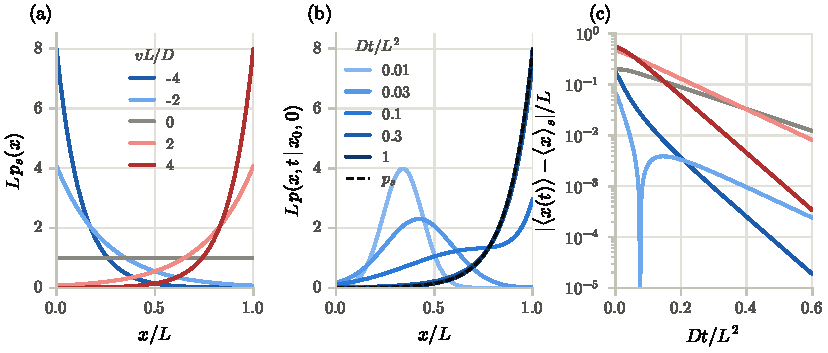
\includegraphics[width=\linewidth]{drift_reflecting.pdf}
  \caption{Constant drift, reflecting walls.
  (a)~Stationary densities for several $vL/D$.
  (b)~Relaxation from $x_0=0.3L$ at $vL/D=4$: the peak is carried to the right wall while it spreads.
  (c)~Distance of the mean from its stationary value, from $x_0=0.3L$; colours as in (a).}
  \label{fig:drift-reflecting}
\end{figure}

% ==============================================================================
\section{Constant drift, absorbing walls}
\label{sec:drift-absorbing}

\begin{keyresults}
$A=v$, $B=D$ on $(0,L)$, $p=0$ at both walls. With $\alpha=v/D=\pm1/\ell$, $\tau=D/v^2$, and $k_n=n\pi/L$:
\begin{align}
  \lambda_n &= \frac1{2\tau}+\frac{n^2\pi^2D}{2L^2},\quad n\ge1,\qquad
  P_n=\sqrt{\frac{2p_s}L}\,\sin k_nx,\quad Q_n=\sqrt{\frac2{Lp_s}}\,\sin k_nx \\
  p(x,t\given x_0,0) &= e^{\alpha(x-x_0)-t/2\tau}\times\text{[free absorbing propagator \cref{eq:A-prop}]} \\
  S(t\given x_0) &= \frac2L\,e^{-\alpha x_0-t/2\tau}\sum_{n\ge1}
  \frac{k_n\bigl[1-(-1)^ne^{\alpha L}\bigr]}{\alpha^2+k_n^2}\,\sin k_nx_0\,e^{-Dk_n^2t/2} \\
  j_0 &= e^{-\alpha x_0-t/2\tau}\,j_0^{\,\text{free}},\qquad j_L=e^{\alpha(L-x_0)-t/2\tau}\,j_L^{\,\text{free}}
  \quad\text{(free fluxes from \cref{eq:A-flux})} \\
  \pi_L(x_0) &= \frac{1-e^{-2\alpha x_0}}{1-e^{-2\alpha L}},\qquad T(x_0)=\frac{L\,\pi_L(x_0)-x_0}{v} \\
  T_L(x_0) &= \frac{L\coth\alpha L-x_0\coth\alpha x_0}{v},\qquad
  T_0(x_0)=\frac{L\coth\alpha L-(L-x_0)\coth\alpha(L-x_0)}{v} \\
  q_\infty(x) &= \frac{\alpha^2+k_1^2}{k_1(1+e^{\alpha L})}\,e^{\alpha x}\sin k_1x,\qquad
  \kappa\to\lambda_1=\frac1{2\tau}+\frac{\pi^2D}{2L^2}
\end{align}
Here $p_s=2\alpha e^{2\alpha x}/(e^{2\alpha L}-1)$ is that of the reflecting interval \G{5.2.91}
(\cref{sec:drift-reflecting}), and $q_\infty=P_1/\int P_1$.
\end{keyresults}

\paragraph{Physical picture.} A slope between two cliffs: the biased gambler's ruin, or a charged molecule
driven by a voltage through a pore and leaving through either end, as in the simplest models of DNA translocation
through a nanopore. $\pi_L$ is the probability of being pushed through rather than falling back.

\paragraph{From Gardiner.} With $\psi=e^{2vx/D}$:
\begin{itemize}
  \item $T$ from \G{5.2.158}, or by solving \G{5.2.154};
  \item $\pi_0,\pi_L$ from the corrected \G{5.2.189}--\G{5.2.190};
  \item $T_0,T_L$ from \G{5.2.183}.
\end{itemize}
A compact general form is $T=\pi_L(x_0)F(L)-F(x_0)$ with
$F(x)=\frac2D\int_0^x\frac{\dd y}{\psi(y)}\int_0^y\psi(z)\,\dd z$. That is the particular solution of
\G{5.2.154} plus a multiple of $\pi_L$, chosen so that $T(L)=0$. Part~III uses the same form.

\subsection{Propagator, survival, fluxes}

Absorbing walls keep $u=0$, so $u$ is exactly the free absorbing propagator and everything follows from
\cref{sec:absorbing}; letting $L\to\infty$ gives back \cref{sec:drift-hl-absorbing}. The $u_n=\sin k_nx$ have
$N_n=L/2$, and \cref{eq:drift-PQ} gives the $P_n$, $Q_n$ of the box: Part~I's $\sqrt2\sin k_nx$, tilted by
$e^{\pm\alpha x}$. Survival uses
$\int_0^Le^{\alpha x}\sin k_nx\,\dd x=k_n[1-(-1)^ne^{\alpha L}]/(\alpha^2+k_n^2)$. Each exit flux is the free one
times $e^{\alpha(w-x_0)}$, which favours the downstream wall, times the common decay $e^{-t/2\tau}$.

\subsection{Splitting probabilities and exit times}

With $\psi=e^{2\alpha x}$, $\pi_L'\propto e^{-2\alpha x}$ (\cref{sec:fpt-toolkit}).
\begin{itemize}
  \item $\pi_L$ is the biased gambler's ruin. For $v>0$ and $L\gg\ell$, $\pi_L\approx1-e^{-2x_0/\ell}$: exit
        is downstream unless the start is within about $\ell/2$ of the upstream wall
        (\cref{fig:drift-absorbing}b).
  \item $T=(L\pi_L-x_0)/v$ solves $vT'+\tfrac12DT''=-1$. For strong drift
        $T\approx(L-x_0)/v$, the transit time (\cref{fig:drift-absorbing}c). The maximum of $T$ moves upstream.
  \item \textbf{Conditional exit times are even in $v$.} Conditioning on exit at $L$ is a Doob transform with
        $h=\pi_L$. It replaces the drift by $v+D\,\partial_x\ln\pi_L=v\coth\alpha x$, which is even in $v$. So the
        paths that leave through $L$ have the same statistics whether the drift helps or opposes them
        (\cref{fig:drift-absorbing}d). Girsanov says the same: the likelihood ratio between drifts $v$ and
        $-v$ for a path exiting at $L$ is $e^{2\alpha(L-x_0)}$, independent of when it exits. As $v\to0$ these
        reduce to $T_L=(L^2-x_0^2)/3D$ and $T_0=x_0(2L-x_0)/3D$.
\end{itemize}

\subsection{Long times}

The QSD is the sine tilted by $e^{\alpha x}$ (this is the preset \texttt{walls} in \texttt{sde-explorer}).
For $L\gg\ell$ it piles up against the downstream wall in a layer of width about $\ell$, and
$\lambda_1\approx1/2\tau$. Starting from the QSD, $T$ is exponential with mean $1/\lambda_1$; the check
$\int q_\infty T\,\dd x_0=1/\lambda_1$ holds for every $v$.

\begin{figure}[tbp]
  \centering
  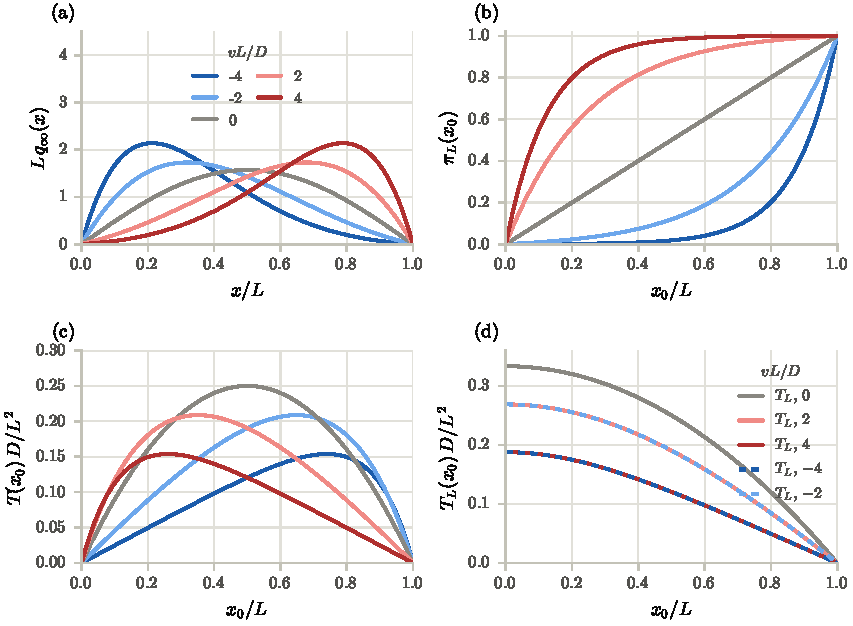
\includegraphics[width=\linewidth]{drift_absorbing.pdf}
  \caption{Constant drift, absorbing walls; colours as in (a) throughout.
  (a)~Quasi-stationary densities.
  (b)~Probability of leaving through $L$.
  (c)~Mean exit time.
  (d)~Mean exit time given exit through $L$. Dashed curves ($v<0$) lie exactly on the solid ones with the
  opposite drift.}
  \label{fig:drift-absorbing}
\end{figure}

% ==============================================================================
\section{Constant drift, reflecting at 0, absorbing at \texorpdfstring{$L$}{L}}
\label{sec:drift-mixed}

\begin{keyresults}
$A=v$, $B=D$ on $(0,L)$, $J=0$ at $x=0$, $p=0$ at $x=L$. With $\alpha=v/D=\pm1/\ell$ and $\tau=D/v^2$:
\begin{align}
  u_n &= \cos k_nx+\frac{\alpha}{k_n}\sin k_nx,\qquad k_n\cos k_nL+\alpha\sin k_nL=0,\qquad
  \lambda_n=\frac1{2\tau}+\tfrac12Dk_n^2 \label{eq:DM-k}\\
  u_0 &= \cosh\kappa x+\frac{\alpha}{\kappa}\sinh\kappa x,\qquad
  \kappa\cosh\kappa L+\alpha\sinh\kappa L=0\qquad\text{if } v<0,\ L>\ell, \notag\\
  \lambda_0 &= \frac1{2\tau}-\tfrac12D\kappa^2 \quad\text{(bound state)} \label{eq:DM-bound}\\
  P_n &= \sqrt{\frac{p_s}{N_n}}\,u_n,\quad Q_n=\frac{u_n}{\sqrt{N_np_s}},\quad N_n=\int_0^Lu_n^2\,\dd x,\quad
  p_s\ \text{of \cref{sec:drift-reflecting}} \\
  p(x,t\given x_0,0) &= \sum_nP_n(x)\,Q_n(x_0)\,e^{-\lambda_nt}=e^{\alpha(x-x_0)}\sum_n\frac{u_n(x)\,u_n(x_0)}{N_n}\,e^{-\lambda_nt} \\
  T(x_0) &= \frac1v\Bigl[(L-x_0)+\frac{e^{-2\alpha L}-e^{-2\alpha x_0}}{2\alpha}\Bigr] \\
  \lambda_0 &\simeq \frac1{T}\simeq\frac2\tau\,e^{-2L/\ell}\qquad(v<0,\ L\gg\ell:\ \text{Arrhenius})
\end{align}
\end{keyresults}

\paragraph{Physical picture.} For $v<0$, a particle held against a floor by gravity in a container whose rim, at
height $L$, is a cliff: to escape it must climb $FL$, an activated escape over a linear barrier. For $v>0$ the force
carries it over the rim. The same geometry describes an ion crossing a membrane against a field into a sink.

\paragraph{From Gardiner.} \G{5.2.160} with $\psi=e^{2vx/D}$ integrates in closed form to the boxed $T$. The
eigenvalue condition comes from \G{5.2.69} at $0$ and \G{5.2.67} at $L$, imposed on $Q_n$; $P_n=p_sQ_n$ with the
reflecting $p_s$ \G{5.2.91}. \Gs{5.2.7c}
(\G{5.2.162}--\G{5.2.174}) is Gardiner's escape problem. Note that there he writes
$\partial_tp=\partial_x(U'p)+D\,\partial_x^2p$, so his $D$ is our $D/2$: his Arrhenius factor
$e^{\Delta U/D}$ \G{5.2.174} is our $e^{2\Delta U/D}$.

\subsection{Spectrum}

Now the Robin condition of \cref{sec:drift-hl-reflecting} at $0$ meets a Dirichlet condition at $L$, so the $k_n$ solve the transcendental
\cref{eq:DM-k}, $\tan k_nL=-k_n/\alpha$. The roots move as the drift changes:
\begin{itemize}
  \item $v>0$ (toward the absorbing wall): $k_nL\in\bigl((n-\tfrac12)\pi,n\pi\bigr)$, $n\ge1$; the
        ground state sits just above $1/2\tau$.
  \item $v=0$: $k_nL=(n+\tfrac12)\pi$, \cref{sec:mixed}.
  \item $v<0$, $L<\ell$: the lowest root falls toward $k=0$, reached at $L=\ell$ with $u_0=1-x/L$.
  \item $v<0$, $L>\ell$: the lowest root moves onto the imaginary axis, $k=i\kappa$, giving the bound state
        \cref{eq:DM-bound} with $\lambda_0<1/2\tau$. Its rate falls exponentially with $L/\ell$
        (\cref{fig:drift-mixed}b). The bound state exists once the interval is longer than the drift length.
\end{itemize}
The eigenfunctions $u_n$ are orthogonal in $L^2$ (Robin plus Dirichlet is self-adjoint), so
\cref{eq:gauge-modes} applies; the script finds the roots numerically.

\subsection{Exit time and escape over a barrier}

\G{5.2.160} with $\psi=e^{2\alpha x}$ gives
$T=\frac2D\int_{x_0}^L\dd y\,e^{-2\alpha y}\int_0^ye^{2\alpha z}\dd z$, which integrates to the boxed form. At
$v=0$ it is $(L^2-x_0^2)/D$.
\begin{itemize}
  \item $v>0$: $T\approx(L-x_0)/v$, the transit time.
  \item $v<0$: the particle sits in the well $U=|v|x$ against the reflecting wall and must climb
        $\Delta U=|v|L$ to escape. Since $p_s\propto e^{-2U/D}$, $\tfrac12D$ plays the role of $k_BT$, so
        $2\Delta U/D=2L/\ell$ and $T\simeq\tfrac12\tau\,e^{2L/\ell}$. This is independent of $x_0$ except within
        about $\ell$ of $L$ (\cref{fig:drift-mixed}c). It is Gardiner's escape problem \Gs{5.2.7c} for a linear
        potential, and here it is exact.
  \item In the same regime $\kappa\to1/\ell$, $\lambda_0\to1/T$, and the QSD becomes the barometric
        profile of \cref{sec:drift-reflecting}, cut off near $L$ (\cref{fig:drift-mixed}a). At $L=4\ell$:
        $\lambda_0=0.010786$, $1/T(0)=0.010767$, and $(2/\tau)e^{-2L/\ell}=0.010735$ (all in $D/L^2$).
\end{itemize}

\begin{figure}[tbp]
  \centering
  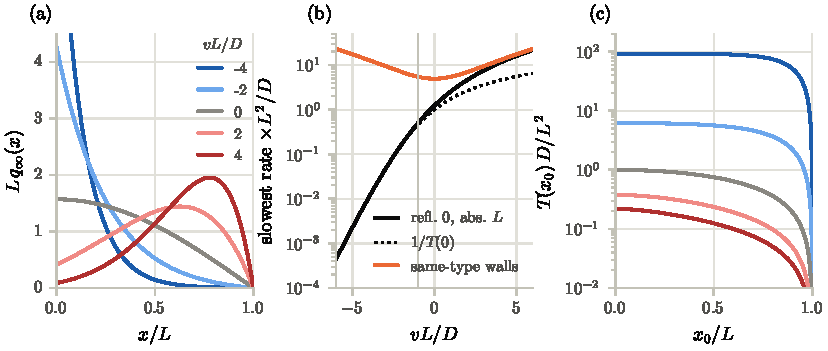
\includegraphics[width=\linewidth]{drift_mixed.pdf}
  \caption{Constant drift, reflecting at $0$, absorbing at $L$.
  (a)~Quasi-stationary densities.
  (b)~Slowest decay rate against $vL/D=\pm L/\ell$; the grey line marks $L=\ell$ with $v<0$, where the bound
  state appears. For comparison, the orange curve is the gap $1/2\tau+\pi^2D/2L^2$, shared by the two
  same-type intervals; the dotted curve is $1/T(0)$.
  (c)~Mean exit time (log scale); colours as in (a).}
  \label{fig:drift-mixed}
\end{figure}

% ==============================================================================
\section{Constant drift on the circle}
\label{sec:drift-circle}

\begin{keyresults}
$A=v$, $B=D$ on the circle of circumference $L$: an overdamped rotor driven by a constant torque. With
$\ell=D/|v|$, $\tau=D/v^2$, $q_m=2\pi m/L$, and $p_{\rm free}$ the propagator \cref{eq:C-prop}:
\begin{align}
  p(x,t\given x_0,0) &= p_{\rm free}(x-vt,t\given x_0,0)
  =\frac1L+\frac2L\sum_{m\ge1}\cos q_m(x-x_0-vt)\,e^{-Dq_m^2t/2} \\
  \lambda_m &= \tfrac12Dq_m^2+ivq_m,\ \ m\in\mathbb Z\ \text{(complex pairs)},\qquad
  \text{gap }\operatorname{Re}\lambda_{\pm1}=\frac{2\pi^2D}{L^2}\ \text{for every }v \\
  P_m &= \frac{e^{iq_mx}}L,\quad Q_m=e^{-iq_mx}\quad\text{(as for $v=0$)},\qquad P_m\neq p_sQ_m \\
  p_s &= \frac1L,\qquad J_s=\frac vL\neq0,\qquad \Phi=\frac{2vL}{D}=\pm\frac{2L}{\ell}\quad\text{(NESS)} \\
  v_{\rm w} &= v,\qquad D_{\rm eff}=D,\qquad \text{entropy production }\frac{2v^2}{D}=\frac2\tau \\
  T_{\rm w} &= \frac{L}{|v|}\tanh\frac L\ell;\qquad
  \text{to a target: }\pi_L,\ T\ \text{of \cref{sec:drift-absorbing} with }x_0\to d
\end{align}
\end{keyresults}

\paragraph{Physical picture.} An overdamped rotor driven by a constant torque: a colloid pushed around a
ring-shaped optical trap by a constant force~\cite{blickle}, or a paddle wheel turned steadily in a viscous fluid.
The steady state is uniform but carries a current; the work done by the torque is dissipated as heat, at the
entropy-production rate $2/\tau$ (in units of $k_B$).

\paragraph{From Gardiner.} \G{5.2.44}--\G{5.2.47} with $\psi=e^{2vx/D}$ and $B=D$: \G{5.2.47} gives
$p_s=p_s(a)$, uniform, and the corrected \G{5.2.46} gives $J=v/L$; as printed it gives $-2v/L$
(\cref{sec:circle-toolkit}). The propagator is the drifting Gaussian \G{3.8.58} summed over the lifts
\cref{eq:cover}, or its characteristic function at $s=q_m$. $T_{\rm w}$ is the $T=(L'\pi_{L'}-x_0)/v$ of
\cref{sec:drift-absorbing} on the cover, with $L'=2L$ and $x_0=L$.

\subsection{The gauge fails; a boost works}

The reduction of Part~II to Part~I, \cref{eq:gauge}, multiplies by $e^{\alpha(x-x_0)}$. That is not a function
on the circle: going once around multiplies it by $e^{\alpha L}$. In the language of
\cref{sec:circle-toolkit}, $2A/B=2\alpha$ is not the derivative of a function on the circle; its period is
$\Phi=2\alpha L\neq0$. One can still gauge, but then $u$ lives on a \emph{twisted} circle,
$u(x+L)=e^{-\alpha L}u(x)$, not on the circle of Part~I (the script checks this).

What works instead is the Galilean boost $x\to x-vt$ that \cref{sec:drift-line} mentioned for the line. There it
was useless once a wall appeared, because the wall does not move. A rotation is a symmetry of the circle and
there is no wall to break it, so $p(x,t\given x_0,0)=p_{\rm free}(x-vt,t\given x_0,0)$ exactly: in the rotating
frame the drift is gone (\cref{fig:drift-circle}a). The circle is the only bounded domain in these notes on which
a change of frame removes the drift.

\subsection{Spectrum: complex, with the gap unchanged}

\begin{itemize}
  \item Translations still commute with the generator, so the Fourier modes are still eigenfunctions. Their
        eigenvalues $\tfrac12Dq_m^2+ivq_m$ are complex: mode $m$ decays and rotates at $m$ times the
        revolution frequency $2\pi v/L$ (\cref{fig:drift-circle}b). The doublet of \cref{sec:circle} becomes a
        complex-conjugate pair, the rotating waves $e^{\pm iq_m(x-vt)}$. Since $A=v$ is odd under no reflection,
        the circle no longer folds into intervals.
  \item The real parts do not depend on $v$. Relaxation goes at $2\pi^2D/L^2$ whatever the drift, because the
        drift only rotates the density. On an interval drift raised every rate by $1/2\tau$
        (\cref{sec:drift-gauge}), because the walls make the density pile up against them.
  \item The generator is not self-adjoint, but it is normal: the Fourier modes are orthonormal in plain $L^2$.
        So the transient of \cref{sec:drift-gauge}, in which the slowest mode can take a transit time to
        dominate, does not occur.
  \item Gardiner's $P_m$ and $Q_m$ are the Fourier modes of the free circle, unchanged; only $\lambda_m$ moves.
        \G{5.2.79} holds, but $P_m=p_sQ_m$ does not, since \G{5.2.71}--\G{5.2.72} need $J_s=0$. What holds instead is
        $P_m=p_s\overline{Q_m}$: forward and backward modes are complex conjugates, as for a normal operator. The
        backward modes are rotating waves
        too: $\avg{e^{-iq_mx(t)}}=Q_m(x_0)\,e^{-\lambda_mt}$, rotating at $v$.
\end{itemize}

\subsection{A steady state with a current}

The stationary density is uniform, exactly as in \cref{sec:circle}, yet this is not equilibrium: $J_s=v/L$
flows forever, because $\Phi=2L/\ell\neq0$. Nothing in $p_s$ reveals the current. It shows up in the winding,
$v_{\rm w}=LJ_s=v$ \cref{eq:winding}, and in the dissipation: the drift does work against friction at rate
$vv_{\rm w}$, and
dividing by the effective temperature $D/2$ gives the entropy production rate $2v^2/D=2/\tau$. The same drift
has no steady state on the line, and on an interval it gives the barometric $p_s$ with $J=0$
(\cref{sec:drift-reflecting}). Only the circle lets it flow.

\subsection{Winding and first passage}

\begin{itemize}
  \item The lift is the drifting Gaussian of \cref{sec:drift-line}, so $v_{\rm w}=v$ and $D_{\rm eff}=D$.
  \item The first full winding is, on the cover, the absorbing interval of length $2L$ of
        \cref{sec:drift-absorbing}, started in the middle. It gives $T_{\rm w}=(L/|v|)\tanh(L/\ell)$, and a
        winding in the direction of the drift with probability $(1+e^{-2L/\ell})^{-1}$. The renewal argument
        then gives $v_{\rm w}=L\tanh(vL/D)/T_{\rm w}=v$, as it must. For $L\gg\ell$, $T_{\rm w}\to L/|v|$, the
        revolution time; for $L\ll\ell$, $T_{\rm w}\to L^2/D$ (\cref{sec:circle}).
  \item First passage to a target: cut there to get \cref{sec:drift-absorbing} with $x_0\to d$. For strong
        drift $v>0$ the target is reached from below, after travelling $L-d$ in a time $T\approx(L-d)/v$,
        unless the start is within about $\ell/2$ above it (\cref{fig:drift-circle}c).
\end{itemize}

\begin{figure}[tbp]
  \centering
  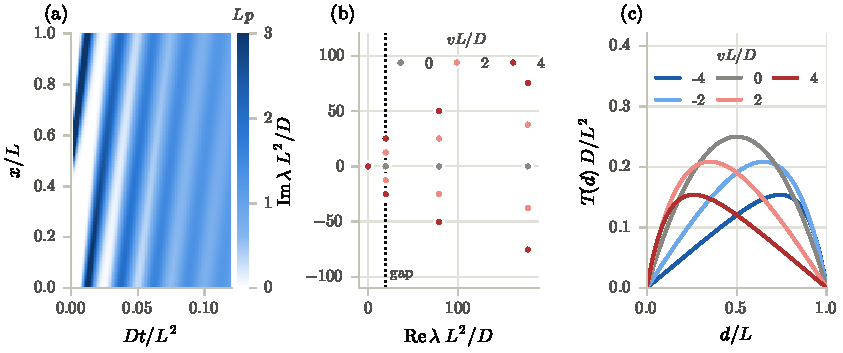
\includegraphics[width=\linewidth]{drift_circle.pdf}
  \caption{Constant drift on the circle.
  (a)~Density against time for $vL/D=40$, from $x_0=L/2$: the peak winds around while it spreads, a helix on
  the cylinder $S^1\times\mathbb R_t$.
  (b)~Eigenvalues $\lambda_m$, $|m|\le3$, in the complex plane. Drift moves them vertically but not
  horizontally, so the gap (dotted) does not depend on $v$. Reversing $v$ gives the same set.
  (c)~Mean time to reach a target from a distance $d$ above it, measured in the $+x$ direction.}
  \label{fig:drift-circle}
\end{figure}

% ==============================================================================
\section{Summary of constant drift}
\label{sec:drift-summary}

\begin{table}[h]
\centering
\small
\renewcommand{\arraystretch}{1.35}
\begin{tabular}{@{}l l l@{}}
\toprule
Walls & Slowest rate & Long times \\
\midrule
reflecting $0$, $L$   & $\frac1{2\tau}+\frac{\pi^2D}{2L^2}$ (gap) & $p_s\propto e^{2vx/D}$ \\
absorbing $0$, $L$    & $\frac1{2\tau}+\frac{\pi^2D}{2L^2}$       & QSD $\propto e^{vx/D}\sin\frac{\pi x}{L}$ \\
refl.\ $0$, abs.\ $L$ & root of \cref{eq:DM-k}, or bound state if $v<0$, $L>\ell$ & $\lambda_0\simeq\frac2\tau e^{-2L/\ell}$ for $v<0$, $L\gg\ell$ \\
reflecting $0$ only   & $1/2\tau$ (gap) if $v<0$; none if $v\ge0$  & $p_s=\frac2\ell e^{-2x/\ell}$ if $v<0$ \\
absorbing $0$ only    & edge $1/2\tau$ if $v<0$                     & QSDs $\lambda\le\frac1{2\tau}$; point start: $\frac{x}{\ell^2}e^{-x/\ell}$ \\
none                  & ---                                         & $g(x-x_0-vt)$ \\
circle                & $\frac{2\pi^2D}{L^2}$ (gap of $\operatorname{Re}\lambda$), complex pairs & $p_s=1/L$ with $J_s=v/L$ (NESS) \\
\bottomrule
\end{tabular}
\caption{Constant drift $A=v$, $B=D$, in every geometry, with $\ell=D/|v|$ and $\tau=D/v^2$.}
\label{tab:drift-summary}
\end{table}

\begin{itemize}
  \item The dynamics sets the scales $\ell=D/|v|$ and $\tau=D/v^2$. Lengths $L$ and $x_0$ only enter as
        $L/\ell$ and $x_0/\ell$. Long-time objects ($p_s$, the half-line QSD, the gap $1/2\tau$) depend on
        $\ell$ and $\tau$ alone; $x_0$ shapes only transients and first passage.
  \item Absorbing walls commute with the gauge, so drift only multiplies free results by
        $e^{\alpha(x-x_0)-t/2\tau}$. Reflecting walls turn into Robin conditions, $u'=\pm u/\ell$, which can
        create a bound state (the barometric $p_s$, or the Arrhenius ground state of the mixed interval).
  \item Drift adds $1/2\tau$ to every rate of the continuum; with two same-type walls this is the whole effect
        on the spectrum, symmetric in $v$.
  \item With one absorbing and one reflecting wall the sign of $v$ matters enormously. Drift toward the
        absorbing wall gives transit, $T\approx(L/\ell)\,\tau$; drift away gives activated escape,
        $T\simeq\tfrac12\tau\,e^{2L/\ell}$.
  \item On the half-line, drift toward the wall turns the free algebraic behaviour into a gap: a stationary
        state with a reflecting wall, a continuum of QSDs with an absorbing one. Drift away gives escape to
        infinity.
  \item Exit statistics conditioned on the exit wall do not depend on the sign of $v$ (Doob/Girsanov).
  \item On the circle the gauge fails, because its factor is not periodic, and a boost removes the drift
        instead. The gap does not depend on $v$, and the uniform $p_s$ carries a current $v/L$.
\end{itemize}


% ==============================================================================
\part{Linear drift: Ornstein--Uhlenbeck, \texorpdfstring{$A=-kx$, $B=D$}{A=-kx, B=D}}
\label{part:ou}

\section{Ornstein--Uhlenbeck: scales and the map to free diffusion}
\label{sec:ou-map}

The equation is $\partial_tp=\partial_x(kxp)+\tfrac12D\,\partial_x^2p$ \G{3.8.61}, from
$\dd x=-kx\,\dd t+\sqrt D\,\dd W$ \G{4.4.22}: overdamped motion in the well $U=\tfrac12kx^2$. All walls in this
part are placed relative to the bottom of the well at $x=0$.

\paragraph{Physical picture.} A harmonic trap, $\mathcal U=\tfrac12\mathcal Kx^2$ with $k=\mathcal K/\gamma$: a bead in
an optical tweezer, an AFM cantilever in liquid, or any overdamped spring. The same equation also describes the
velocity of a free Brownian particle, which is where Ornstein and Uhlenbeck started: there $x$ is the velocity and
$k=\gamma/m$ \G{6.4.2}--\G{6.4.3}.

\paragraph{From Gardiner.} The book solves this process three ways, and each is used below.
\begin{itemize}
  \item \Gs{3.8.4} uses the characteristic function: the first-order equation \G{3.8.63} is solved by
        characteristics to give \G{3.8.71}, a Gaussian.
  \item \Gs{4.4.4} solves the SDE directly with the substitution $y=xe^{kt}$ \G{4.4.23}, which removes the
        drift, $\dd y=\sqrt De^{kt}\dd W$ \G{4.4.25}. This gives the mean, the variance and the correlation
        function \G{4.4.26}--\G{4.4.30}.
  \item \Gs{5.2.6c} gives the eigenfunctions: Hermite polynomials \G{5.2.115}--\G{5.2.122}, with $\lambda=nk$
        \G{5.2.119} and $p_s$ \G{5.2.120}.
\end{itemize}

\paragraph{Scales.} As in Part~II, the dynamics fixes a length and a time,
\begin{equation}
  \ell\equiv\sqrt{D/k},\qquad \tau\equiv1/k,\qquad \ell^2=D\tau,\qquad \xi\equiv x/\ell .
  \label{eq:ou-scales}
\end{equation}
The stationary variance is $D/2k=\ell^2/2$, so $p_s=e^{-\xi^2}/(\ell\sqrt\pi)$. A wall at distance $L$ from the
bottom sits at height $\Delta U=\tfrac12kL^2$, and $\Delta U/(D/2)=(L/\ell)^2$: $\xi^2$ measures energy in
units of the ``temperature'' $D/2$.

\paragraph{The map.} Gardiner's substitution turns OU into free diffusion with $B=D$, run on the clock
$\theta(t)=\int_0^te^{2ks}\,\dd s=(e^{2kt}-1)/2k$. A wall at $x=0$ stays at $y=0$, so for any walls at the
bottom of the well
\begin{equation}
  p_{\text{OU}}(x,t\given x_0,0)=e^{kt}\,p_{\text{free}}\bigl(e^{kt}x,\theta(t)\given x_0,0\bigr),
  \label{eq:ou-map}
\end{equation}
with $p_{\text{free}}$ taken from Part~I with the same walls. For $t\ll\tau$, $\theta\approx t$ and OU looks
free. For $t\gg\tau$ the free spreading $\sqrt{D\theta}\propto e^{kt}$ is exactly cancelled by the factor
$e^{-kt}$: this is how a confining force turns algebraic spreading into a stationary state. A wall at
$x=a\neq0$ moves under the map ($y=ae^{kt}$), so the intervals of
\cref{sec:ou-reflecting,sec:ou-absorbing,sec:ou-mixed} need eigenfunctions instead.

\paragraph{Eigenfunctions.} In the variable $\xi$, the backward eigen-equation is Hermite's equation, as in
Gardiner's \G{5.2.116} and \G{5.2.117}:
\begin{equation}
  Q''-2\xi Q'+2\nu Q=0,\qquad \lambda=\nu k,
\end{equation}
whose even and odd solutions for any $\nu$ are Kummer functions,
\begin{equation}
  Q_{\text{even}}=M\bigl(-\tfrac\nu2,\tfrac12,\xi^2\bigr),\qquad
  Q_{\text{odd}}=\xi\,M\bigl(\tfrac{1-\nu}2,\tfrac32,\xi^2\bigr).
  \label{eq:kummer}
\end{equation}
On the line, normalisability forces $\nu=n$ and the Hermite polynomials \G{5.2.118}. With walls, the wall
conditions fix $\nu$. The eigenfunctions are orthogonal with weight $p_s\propto e^{-\xi^2}$, and Gardiner's forward
eigenfunctions are $P=p_sQ$. On every interval of this part $p_s$ is the truncated half-Gaussian of the reflecting
interval (\cref{sec:ou-reflecting}), also when a wall absorbs \G{5.2.91}, and $Q_n$ is normalised by
$\int p_sQ_n^2\,\dd x=1$ \G{5.2.80}. In the symmetrised
form of \cref{sec:operator} this is the harmonic oscillator, $V=\tfrac12k(\xi^2-1)$
(\cref{fig:operators}a).

\paragraph{A ladder.} Differentiate the backward eigen-equation $A\,Q'+\tfrac12DQ''=-\lambda Q$: with
$A'=-k$ constant, $Q'$ obeys the same equation with $\lambda\to\lambda-k$. On the line this is the Hermite
ladder $H_n'=2nH_{n-1}$. With walls, a reflecting eigenfunction has $Q'=0$ at the walls, so its derivative is an
absorbing eigenfunction: \emph{the reflecting spectrum is the absorbing spectrum shifted up by $k$}, plus
$\lambda=0$. For constant $A$ (Parts~I and~II) the shift is zero, which is why the reflecting and absorbing
intervals there share their nonzero eigenvalues.

% ==============================================================================
\section{Ornstein--Uhlenbeck on the whole line}
\label{sec:ou-line}

\begin{keyresults}
$A=-kx$, $B=D$ on $(-\infty,\infty)$; $\ell=\sqrt{D/k}$, $\tau=1/k$, $\xi=x/\ell$.
\begin{align}
  p(x,t\given x_0,0) &= \text{Gaussian},\quad \avg x=x_0e^{-t/\tau},\quad
  \operatorname{Var}x=\tfrac12\ell^2\bigl(1-e^{-2t/\tau}\bigr) \\
  &= \frac{e^{-\xi^2}}{\ell\sqrt\pi}\sum_{n\ge0}\frac{H_n(\xi)H_n(\xi_0)}{2^nn!}\,e^{-nt/\tau}
  \quad\text{(Mehler)} \label{eq:ou-mehler}\\
  \lambda_n &= nk,\quad Q_n=\frac{H_n(\xi)}{\sqrt{2^nn!}},\quad P_n=p_sQ_n,\quad p_s=\frac{e^{-x^2/\ell^2}}{\ell\sqrt\pi},
  \quad\text{gap }k \\
  C(t) &= \avg{x(t)x(0)}_s=\tfrac12\ell^2e^{-|t|/\tau}\quad\text{(exactly one exponential)}
\end{align}
\end{keyresults}

\paragraph{Physical picture.} A bead in an optical tweezer. Its stationary variance $\ell^2/2=k_BT/\mathcal K$
(equipartition) and its relaxation rate $k=\mathcal K/\gamma$ are the two standard ways of calibrating the trap
stiffness; the rate appears as the corner frequency $\mathcal K/2\pi\gamma$ of the position power spectrum.

\paragraph{From Gardiner.} The Gaussian is \G{3.8.71} inverted, or \G{4.4.26} with the moments
\G{4.4.27}--\G{4.4.29}. $Q_n$ is his \G{5.2.118}, normalised as in \G{5.2.79}--\G{5.2.81}, and $p_s$ is \G{5.2.120}
(our $\xi$ is his $x\sqrt{k/D}$). The expansion \cref{eq:ou-mehler} is \G{5.2.121} with the coefficients \G{5.2.122}
evaluated for a sharp start, and $C(t)$ is the stationary limit of \G{4.4.30}: only $P_1$ has $\int xP_n\ne0$
\G{5.2.125}.

\subsection{From the free line}

Put the Gaussian of \cref{sec:line} through \cref{eq:ou-map}: the mean $x_0$ becomes $x_0e^{-kt}$, and the
variance $D\theta$ becomes $D\theta e^{-2kt}=\tfrac12\ell^2(1-e^{-2kt})$. That is the whole solution; the Mehler
sum is the same function written in eigenfunctions (they agree to $10^{-15}$).

\subsection{Gap and moments}

\begin{itemize}
  \item The gap is $k$, independent of $D$. In the Rayleigh quotient \cref{eq:rayleigh} the slowest
        function is $f=x$, and its cost is set by the curvature of the well. Noise sets only the width $\ell$.
  \item $x\propto H_1$ has overlap with mode $1$ only, so $\avg{x(t)}=x_0e^{-kt}$ exactly, and
        $C(t)\propto e^{-k|t|}$ is a single exponential. Compare the reflecting interval, where the slowest
        mode carried $98.6\,\%$ (\cref{sec:reflecting}).
  \item $x^2$ is a combination of $H_0$ and $H_2$, so
        $\avg{x^2}-\tfrac12\ell^2=(x_0^2-\tfrac12\ell^2)e^{-2kt}$: it relaxes at $2k$, faster than the gap.
        This is the symmetry selection of \cref{sec:gap} (\cref{fig:ou-line}b).
\end{itemize}

\begin{figure}[tbp]
  \centering
  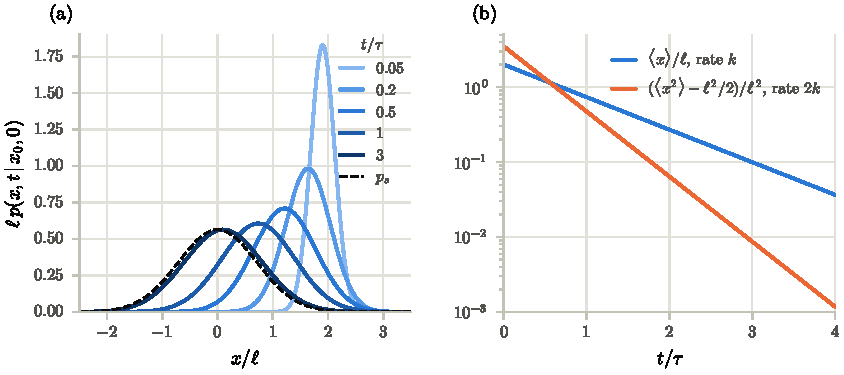
\includegraphics[width=\linewidth]{ou_line.pdf}
  \caption{Ornstein--Uhlenbeck on the line, from $x_0=2\ell$; units $\ell=\sqrt{D/k}$, $\tau=1/k$.
  (a)~The Gaussian slides to the origin while widening to $p_s$.
  (b)~$\avg x$ relaxes at the gap $k$; the second moment, with no overlap on mode $1$, at $2k$.}
  \label{fig:ou-line}
\end{figure}

% ==============================================================================
\section{Ornstein--Uhlenbeck on the half-line, reflecting at the bottom}
\label{sec:ou-hl-reflecting}

\begin{keyresults}
$A=-kx$, $B=D$ on $(0,\infty)$, $J=0$ at $x=0$, the bottom of the well. With $m_t=x_0e^{-t/\tau}$ and
$\sigma_t^2=\tfrac12\ell^2(1-e^{-2t/\tau})$:
\begin{align}
  p(x,t\given x_0,0) &= G_{\sigma_t}(x-m_t)+G_{\sigma_t}(x+m_t),\qquad
  G_\sigma(y)=\frac{e^{-y^2/2\sigma^2}}{\sqrt{2\pi}\,\sigma} \label{eq:ouhr-prop}\\
  p_s(x) &= \frac{2}{\ell\sqrt\pi}\,e^{-x^2/\ell^2}\ \text{(half-Gaussian)},\qquad \avg x_s=\frac{\ell}{\sqrt\pi} \\
  \lambda_m &= 2mk,\quad Q_m=\frac{H_{2m}(\xi)}{\sqrt{2^{2m}(2m)!}},\quad P_m=p_sQ_m\quad\text{(even Hermite)},
  \quad\text{gap }2k \\
  \avg{x^2(t)} &= x_0^2e^{-2t/\tau}+\tfrac12\ell^2\bigl(1-e^{-2t/\tau}\bigr)\quad\text{(exact, as on the line)}
\end{align}
\end{keyresults}

\paragraph{Physical picture.} A trapped bead whose trap centre sits exactly on a hard surface, such as a
coverslip at the focus of an optical tweezer. It explores only one half of the trap, so its density is a
half-Gaussian.

\paragraph{From Gardiner.} The wall is \G{5.2.13} at $x=0$. Of the Hermite eigenfunctions \G{5.2.118}, only
the even ones satisfy the reflecting backward condition \G{5.2.69}, $H_n'(0)=0$, which gives the spectrum.
$p_s$ is \cref{eq:ps} restricted to $x>0$.

\subsection{From the free half-line}

The wall sits at the fixed point of the map, so \cref{eq:ou-map} applied to the image pair of
\cref{sec:hl-reflecting} gives \cref{eq:ouhr-prop} directly: the source and its mirror image each turn into
the OU Gaussian. Where the free half-line spread forever with no stationary state, the well freezes the
spreading into the half-Gaussian.

\subsection{Gap}

The reflecting wall removes the odd modes, including the line's slowest one, $H_1$. The surviving $Q_m$ are the
line's, normalisation included; $P_m=p_sQ_m$ is twice the line's $P_{2m}$, because $p_s$ is. The gap doubles to $2k$,
and now even $\avg x$ relaxes at $2k$ (\cref{fig:ou-hl-reflecting}b). The second moment is unchanged by the
wall, for the reason given in \cref{sec:hl-reflecting}: $x^2$ is even.

\begin{figure}[tbp]
  \centering
  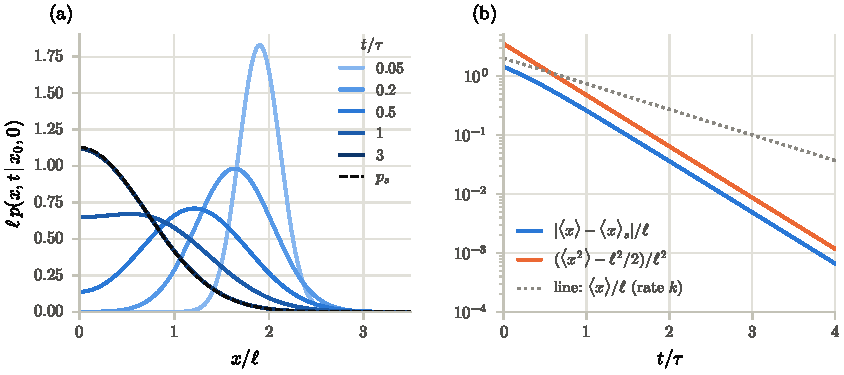
\includegraphics[width=\linewidth]{ou_halfline_reflecting.pdf}
  \caption{OU with a reflecting wall at the bottom of the well, from $x_0=2\ell$.
  (a)~Relaxation to the half-Gaussian.
  (b)~Both moments relax at $2k$; the dotted line is the line's $\avg x$, which relaxes at $k$.}
  \label{fig:ou-hl-reflecting}
\end{figure}

% ==============================================================================
\section{Ornstein--Uhlenbeck on the half-line, absorbing at the bottom}
\label{sec:ou-hl-absorbing}

\begin{keyresults}
$A=-kx$, $B=D$ on $(0,\infty)$, $p=0$ at $x=0$. With $m_t$, $\sigma_t$ as in \cref{sec:ou-hl-reflecting}:
\begin{align}
  p(x,t\given x_0,0) &= G_{\sigma_t}(x-m_t)-G_{\sigma_t}(x+m_t) \\
  S(t\given x_0) &= \operatorname{erf}\frac{x_0/\ell}{\sqrt{e^{2t/\tau}-1}}
  \;\xrightarrow{\;t\gg\tau\;}\;\frac{2}{\sqrt\pi}\,\frac{x_0}{\ell}\,e^{-t/\tau} \\
  \lambda_m &= (2m+1)k\ \ \text{(odd Hermite): bottom }k,\ \text{gap }2k \\
  Q_m &= \frac{H_{2m+1}(\xi)}{\sqrt{2^{2m+1}(2m+1)!}},\qquad P_m=p_sQ_m \\
  q_\nu(x) &= \frac{2\nu}{\ell}\,\xi\,e^{-\xi^2}M\bigl(\tfrac{1-\nu}2,\tfrac32,\xi^2\bigr)\sim x^{-1-\nu},\qquad
  \lambda=\nu k,\quad 0<\nu\le1 \\
  q(x,t) &\to q_1=\frac{2x}{\ell^2}\,e^{-x^2/\ell^2}\ \text{(Rayleigh)},\quad \kappa\to k
  \qquad\text{if }p(x,0)\text{ has a finite mean} \\
  q(x,t) &\to q_\nu,\quad S\propto e^{-\nu t/\tau}\qquad\text{if }p(x,0)\sim x^{-1-\nu},\ 0<\nu<1 \\
  T(x_0) &= \sqrt\pi\,\tau\int_0^{x_0/\ell}\operatorname{erfcx}(u)\,\dd u
  \;\simeq\;\tau\Bigl[\ln\frac{2x_0}{\ell}+\frac{\gamma_{\rm E}}2\Bigr]\quad(x_0\gg\ell)
\end{align}
with $\operatorname{erfcx}(u)=e^{u^2}\operatorname{erfc}u$ and $\gamma_{\rm E}$ Euler's constant. In $P_m$,
$p_s=2e^{-\xi^2}/\ell\sqrt\pi$ is the half-Gaussian of \cref{sec:ou-hl-reflecting} \G{5.2.91}. The $q_\nu$ are a
continuum of QSDs; the tail of the initial density decides which one is reached.
\end{keyresults}

\paragraph{Physical picture.} Any mean-reverting quantity that is stopped the first time it returns to its
mean. Examples are a trapped particle removed by a sticky surface through the trap centre, or a leaky
integrate-and-fire neuron whose threshold sits at its resting potential. The logarithmic $T$ says that the return
from far away is fast and deterministic, and only the last stretch, within $\ell$, is diffusive.

\paragraph{From Gardiner.} $S$ is $G(x_0,t)$ of \G{5.2.140}. The mean exit time is \G{5.2.161} with the
reflecting wall $b$ moved to infinity and $\psi=e^{-x^2/\ell^2}$:
$T=\frac2D\int_0^{x_0}\frac{\dd y}{\psi(y)}\int_y^\infty\psi(z)\,\dd z$, which becomes the erfcx integral. The
odd Hermite functions satisfy the absorbing backward condition \G{5.2.67}, $H_n(0)=0$. The other QSDs are the
odd Kummer functions \cref{eq:kummer} with non-integer $\nu$, which the book does not consider.

\subsection{From the free half-line}

Apply \cref{eq:ou-map} to \cref{sec:hl-absorbing}. The free survival $\operatorname{erf}(x_0/\sqrt{2D\theta})$
becomes the boxed $S$, because $2D\theta=\ell^2(e^{2kt}-1)$. Two of the free half-line's results change
character:
\begin{itemize}
  \item \textbf{QSDs appear.} Mapped back, the free Rayleigh profile $(x/D\theta)\,e^{-x^2/2D\theta}$ has
        width $\sqrt{D\theta}\,e^{-kt}$, which tends to $\ell/\sqrt2$. It stops spreading and freezes into the
        Rayleigh QSD $q_1=(2x/\ell^2)e^{-x^2/\ell^2}$. In spectral terms, the bottom of the spectrum is no longer
        a continuum at $0$ but the isolated level $H_1$ at $k$ (\cref{sec:gap}). This is the QSD reached from a
        point start, but it is not the only one (below).
  \item \textbf{The mean exit time is finite and logarithmic.} From far away the particle relaxes
        deterministically, $x_0e^{-t/\tau}$, until it is within about $\ell$ of the wall, which takes
        $\tau\ln(x_0/\ell)$. Diffusion then finishes the job in a time of order $\tau$. The constant
        $\ln2+\gamma_{\rm E}/2\approx0.98$ is checked numerically.
\end{itemize}

\subsection{A continuum of QSDs, and which one is reached}

\begin{itemize}
  \item \textbf{The family.} For any $\nu$, the forward eigenfunctions are $e^{-\xi^2}$ times the Kummer
        functions \cref{eq:kummer}, and the odd one vanishes at the wall.
        \begin{itemize}
          \item For $0<\nu<1$ it is positive. By Kummer's transformation $e^{-z}M(a,b,z)=M(b-a,b,-z)$ it
                decays as $\xi^{-1-\nu}$, so it is integrable: a QSD $q_\nu$ with decay rate $\nu k$.
          \item The normalisation in the box follows from $\int_0^\infty M(a,b,-z)\,\dd z=(b-1)/(a-1)$.
          \item At $\nu=1$ it is the Rayleigh density; for $\nu>1$ it changes sign.
        \end{itemize}
        None of these is in $L^2$ with the weight $e^{\xi^2}$, which is why the spectrum $(2m+1)k$ does not show
        them. In Gardiner's terms $q_\nu\propto p_sQ$ with $Q=\xi M(\frac{1-\nu}2,\frac32,\xi^2)$, the odd solution of
        \G{5.2.117} for non-integer $\nu$; this $Q$ grows like $e^{\xi^2}\xi^{-1-\nu}$, so $\int P Q$ \G{5.2.79}
        diverges. The same happened for the continuum below the edge in \cref{sec:drift-hl-absorbing}. The script
        checks that $q_\nu$ evolves exactly as $e^{-\nu kt}q_\nu$.
  \item \textbf{Point start, or any start with a finite mean.} Through the map, the free half-line's density
        near the wall is $\propto x\int y\,p(y,0)\,\dd y$ (\cref{sec:hl-absorbing}). That maps back to the
        Rayleigh QSD, which a point start approaches at the gap $2k$.
  \item \textbf{Power-law starts.} If $p(y,0)\sim y^{-1-\nu}$ with $0<\nu<1$, the mean is infinite and the far
        tail dominates. The map turns the integral over the tail into
        $\int_0^\infty z^{-1-\nu}\sinh(wz)\,e^{-z^2/2}\,\dd z$, with $w=\sqrt2\,\xi$. That integral is $w$ times
        a Kummer function of $w^2/2=\xi^2$, so the conditioned density converges to $q_\nu$ and
        $S\propto e^{-\nu kt}$, exactly~\cite{lladser} (\cref{fig:attraction}b).
  \item \textbf{Why.} A particle starting at $y\gg\ell$ needs about $\tau\ln(y/\ell)$ to come down; this is the
        logarithm in $T(x_0)$ above. A tail $y^{-\nu}$ of starting points therefore arrives as $e^{-\nu kt}$,
        which beats the bulk's $e^{-kt}$ when $\nu<1$. Here the rule is exact, because the map is. A tail heavier
        than every power gives no limit: the conditioned density keeps following the incoming tail outward.
  \item The unbounded $T(x_0)$ is also what rules out a unique QSD (\cref{sec:spectrum-states}).
\end{itemize}

\begin{figure}[tbp]
  \centering
  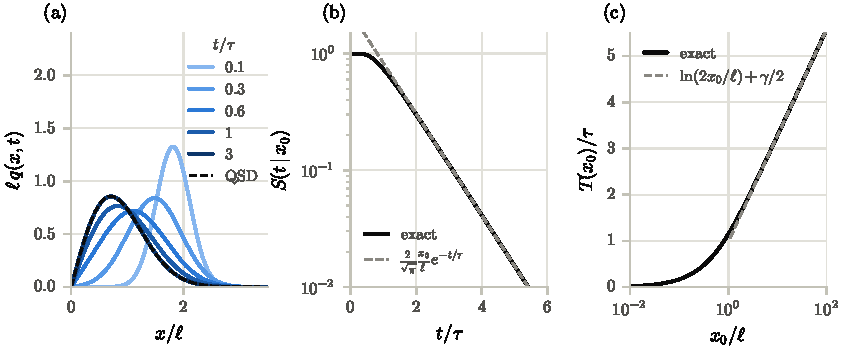
\includegraphics[width=\linewidth]{ou_halfline_absorbing.pdf}
  \caption{OU with an absorbing wall at the bottom of the well, from $x_0=2\ell$.
  (a)~From a point start the conditioned density converges to the Rayleigh QSD; compare \cref{fig:hl-absorbing}b, where the
  same shape kept spreading.
  (b)~Survival decays at $\lambda_{\min}=k$.
  (c)~Mean exit time, with its logarithmic asymptote.}
  \label{fig:ou-hl-absorbing}
\end{figure}

% ==============================================================================
\section{Ornstein--Uhlenbeck on an interval, both walls reflecting}
\label{sec:ou-reflecting}

\begin{keyresults}
$A=-kx$, $B=D$ on $(0,L)$ with $x=0$ at the bottom of the well, $J=0$ at both walls.
\begin{align}
  p_s(x) &= \frac{2\,e^{-x^2/\ell^2}}{\ell\sqrt\pi\,\operatorname{erf}(L/\ell)}\quad\text{(truncated half-Gaussian)} \\
  Q_n &\propto M\bigl(-\tfrac{\nu_n}2,\tfrac12,\xi^2\bigr),\quad Q_n'(L/\ell)=0,\quad P_n=p_sQ_n,\quad \lambda_n=\nu_nk \\
  p(x,t\given x_0,0) &= \sum_nP_n(x)\,Q_n(x_0)\,e^{-\nu_nt/\tau},\quad \int_0^Lp_sQ_n^2\,\dd x=1,\quad \nu_0=0,\ Q_0=1 \\
  \text{gap }\lambda_1 &\to \frac{\pi^2D}{2L^2}\ (L\ll\ell),\qquad \lambda_1\to2k\ (L\gg\ell)
\end{align}
\end{keyresults}

\paragraph{Physical picture.} A trapped bead confined to a channel, with one hard wall at the trap centre and
another at distance $L$. Widening the channel takes it from a box ($L\ll\ell$, where the trap does not matter) to a
trap ($L\gg\ell$, where the far wall does not matter).

\paragraph{From Gardiner.} $p_s$ is \cref{eq:ps} \G{5.2.39}. The eigenfunctions solve
\G{5.2.116}--\G{5.2.117} for non-integer $\nu$, with the reflecting backward condition \G{5.2.69} at both
walls. The expansion is \G{5.2.84}--\G{5.2.88} with $P=p_sQ$ (\G{5.2.71}, \G{5.2.73}--\G{5.2.74}).

\subsection{Adding a second wall}

This is \cref{sec:ou-hl-reflecting} with a second wall at $L$, as \cref{sec:reflecting} was
\cref{sec:hl-reflecting} with a second mirror. The map no longer helps, because the wall at $L$ moves under it.
The even Kummer function \cref{eq:kummer} already satisfies the wall at $0$, and the wall at $L$ quantises
$\nu$; the script finds the roots numerically.

\subsection{Crossover}

\begin{itemize}
  \item For $L\ll\ell$ the potential barely changes across the interval, and the problem is
        \cref{sec:reflecting}: $\lambda_1\approx\pi^2D/2L^2$.
  \item For $L\gg\ell$ the far wall sits where $p_s$ is negligible, and the problem is
        \cref{sec:ou-hl-reflecting}: $\lambda_1\to2k$.
\end{itemize}
In terms of the Rayleigh quotient, the slowest function varies over whichever is shorter, $L$ or $\ell$
(\cref{fig:ou-summary}).

\begin{figure}[tbp]
  \centering
  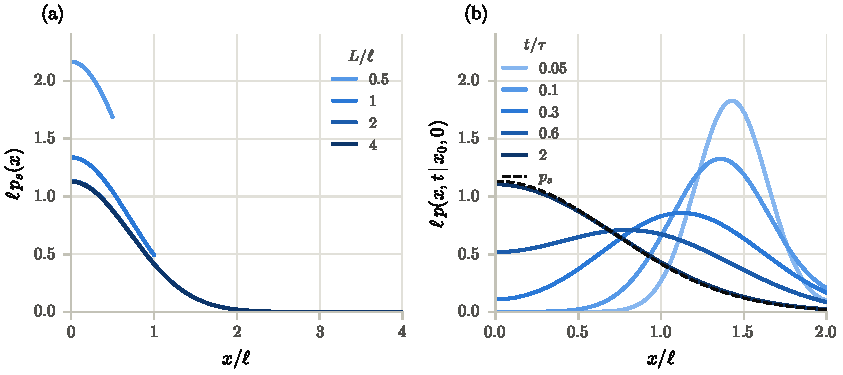
\includegraphics[width=\linewidth]{ou_reflecting.pdf}
  \caption{OU on $(0,L)$ with reflecting walls, $x=0$ at the bottom of the well.
  (a)~Stationary densities, the half-Gaussian truncated at $L$.
  (b)~Relaxation for $L=2\ell$ from $x_0=1.5\ell$.}
  \label{fig:ou-reflecting}
\end{figure}

% ==============================================================================
\section{Ornstein--Uhlenbeck on an interval, both walls absorbing}
\label{sec:ou-absorbing}

\begin{keyresults}
$A=-kx$, $B=D$ on $(0,L)$ with $x=0$ at the bottom of the well, $p=0$ at both walls.
\begin{align}
  Q_n &\propto \xi\,M\bigl(\tfrac{1-\nu_n}2,\tfrac32,\xi^2\bigr),\quad Q_n(L/\ell)=0,\quad P_n=p_sQ_n \\
  \lambda_n &= \nu_nk,\qquad \nu_{n+1}^{\text{refl}}=\nu_n^{\text{abs}}+1 \\
  \pi_L(x_0) &= \frac{\operatorname{erfi}(x_0/\ell)}{\operatorname{erfi}(L/\ell)},\qquad
  T(x_0)=\tau\bigl[\pi_L(x_0)\,G(L/\ell)-G(x_0/\ell)\bigr] \\
  G(\xi) &= \sqrt\pi\int_0^\xi e^{u^2}\operatorname{erf}(u)\,\dd u \\
  \lambda_{\min} &\to \frac{\pi^2D}{2L^2}\ (L\ll\ell),\qquad \lambda_{\min}\to k\ (L\gg\ell);\qquad
  q_\infty\propto P_0\propto e^{-\xi^2}Q_0(\xi)
\end{align}
$p_s$ and the normalisation of $Q_n$ are those of \cref{sec:ou-reflecting} \G{5.2.91}.
\end{keyresults}

\paragraph{Physical picture.} The same channel with sticky ends, one of them at the trap centre. $\pi_L$ is
the probability of reaching the far end against the restoring force: climbing out of a well on a small scale.

\paragraph{From Gardiner.} The absorbing backward condition \G{5.2.67} at both walls selects the odd Kummer
function and quantises $\nu$. With $1/\psi=e^{x^2/\ell^2}$ the corrected \G{5.2.189}--\G{5.2.190} give $\pi_L$
as a ratio of $\int_0^xe^{y^2/\ell^2}\dd y\propto\operatorname{erfi}(x/\ell)$. $T$ is the compact form of
\G{5.2.154}/\G{5.2.158} from \cref{sec:drift-absorbing}, $T=\pi_LF(L)-F(x_0)$, with $F=\tau G$.

\subsection{Building on the earlier sections}

\begin{itemize}
  \item The odd Kummer function vanishes at the bottom wall, as the odd Hermite functions did in
        \cref{sec:ou-hl-absorbing}; the wall at $L$ quantises $\nu$.
  \item The ladder of \cref{sec:ou-map} gives the whole spectrum from \cref{sec:ou-reflecting}: the
        derivative of each reflecting eigenfunction is an absorbing one, with $\nu$ lower by exactly 1. The
        script checks this to $10^{-15}$.
  \item Crossover: for $L\ll\ell$, \cref{sec:absorbing} (sine QSD, $\lambda=\pi^2D/2L^2$); for $L\gg\ell$,
        \cref{sec:ou-hl-absorbing} (Rayleigh QSD, $\lambda=k$) (\cref{fig:ou-absorbing}a, \cref{fig:ou-summary}).
  \item Climbing is hard. For $x_0,L\gg\ell$,
        $\pi_L\approx(L/x_0)\,e^{-(L^2-x_0^2)/\ell^2}$: to leave through $L$ the particle must climb the
        potential, and it almost always falls back to the bottom wall (\cref{fig:ou-absorbing}b).
\end{itemize}

\begin{figure}[tbp]
  \centering
  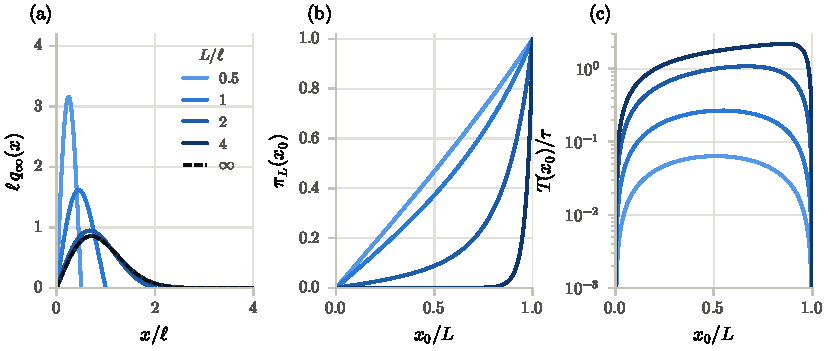
\includegraphics[width=\linewidth]{ou_absorbing.pdf}
  \caption{OU on $(0,L)$ with absorbing walls; colours as in (a).
  (a)~Quasi-stationary densities, from the sine of Part~I ($L\ll\ell$) to the Rayleigh QSD of
  \cref{sec:ou-hl-absorbing} (dashed).
  (b)~Probability of leaving through the upper wall.
  (c)~Mean exit time.}
  \label{fig:ou-absorbing}
\end{figure}

% ==============================================================================
\section{Ornstein--Uhlenbeck: reflecting at the bottom, absorbing at \texorpdfstring{$L$}{L} (escape from a well)}
\label{sec:ou-mixed}

\begin{keyresults}
$A=-kx$, $B=D$ on $(0,L)$, $J=0$ at the bottom $x=0$, $p=0$ at $x=L$.
\begin{align}
  Q_n &\propto M\bigl(-\tfrac{\nu_n}2,\tfrac12,\xi^2\bigr),\quad Q_n(L/\ell)=0,\quad P_n=p_sQ_n,\quad \lambda_n=\nu_nk \\
  T(x_0) &= \tau\bigl[G(L/\ell)-G(x_0/\ell)\bigr] \\
  L\gg\ell:\quad \lambda_0 &\simeq\frac1{T}\simeq\frac{2}{\sqrt\pi\,\tau}\,\frac L\ell
  \Bigl(1-\frac{\ell^2}{2L^2}\Bigr)e^{-L^2/\ell^2}\quad\text{(Kramers)} \\
  L\ll\ell:\quad \lambda_0 &\to \frac{\pi^2D}{8L^2}\quad\text{(\cref{sec:mixed})}
\end{align}
$p_s$ and the normalisation of $Q_n$ are those of \cref{sec:ou-reflecting} \G{5.2.91}.
\end{keyresults}

\paragraph{Physical picture.} Escape from a harmonic well whose rim is a cliff: a bead escaping an optical
trap of finite extent, or a harmonic bond that breaks when stretched beyond $L$, the simplest model of thermally
activated bond rupture. The Arrhenius factor $e^{L^2/\ell^2}=e^{\mathcal KL^2/2k_BT}$ is the Boltzmann factor of the
rim.

\paragraph{From Gardiner.} \G{5.2.160} (``$a$ reflecting, $b$ absorbing'') with $\psi=e^{-x^2/\ell^2}$ gives
$T$ exactly: $T=\frac2D\int_{x_0}^L\frac{\dd y}{\psi(y)}\int_0^y\psi(z)\,\dd z=\tau[G(L/\ell)-G(x_0/\ell)]$.
\Gs{5.2.7c} is the asymptotic analysis of the same integrals, \G{5.2.165}--\G{5.2.174}. The inner integral is
Gaussian about the minimum, as here. Gardiner's barrier is a smooth maximum, which makes the outer integral
Gaussian too and gives the prefactor of \G{5.2.174}. Here the barrier top is the absorbing wall itself, so
the outer integral is cut off at $L$ and contributes $e^{L^2/\ell^2}/(2L/\ell)$ instead. That is the origin of
the $L/\ell$ in the rate.

\subsection{Escape}

\begin{itemize}
  \item This is the mixed interval of Part~I in a harmonic well, and the harmonic version of
        \cref{sec:drift-mixed}. Both have Arrhenius factor $e^{2\Delta U/D}$: $e^{2L/\ell_v}$ for the linear
        potential, with $\ell_v=D/|v|$ the length $\ell$ of Part~II, and $e^{L^2/\ell^2}$ here.
  \item Unfolding, as in \cref{sec:mixed}: a reflecting wall at the bottom of a symmetric well is the full
        well $(-L,L)$ with absorbing walls at both ends. The half-well escape rate is therefore the rate of a
        full well with two exits, twice that of a full well with one.
  \item For $L\gg\ell$, $T$ is the same from every start that is not within about $\ell$ of the exit
        (\cref{fig:ou-mixed}b). The QSD is the half-Gaussian $p_s$ of \cref{sec:ou-hl-reflecting}, cut off
        near $L$ (\cref{fig:ou-mixed}a): $Q_0\approx1$ except within about $\ell$ of the exit, so $P_0=p_sQ_0\approx p_s$. The gap to the next level, about $2k$, is huge compared with
        $\lambda_0$: the particle equilibrates in the well long before it escapes (\cref{fig:spectra}).
  \item The Kramers formula with its first correction matches $\lambda_0$ to $0.1\,\%$ at $L=5\ell$, and
        $\lambda_0T(0)=1.0005$ already at $L=3\ell$ (\cref{fig:ou-mixed}c).
\end{itemize}

\begin{figure}[tbp]
  \centering
  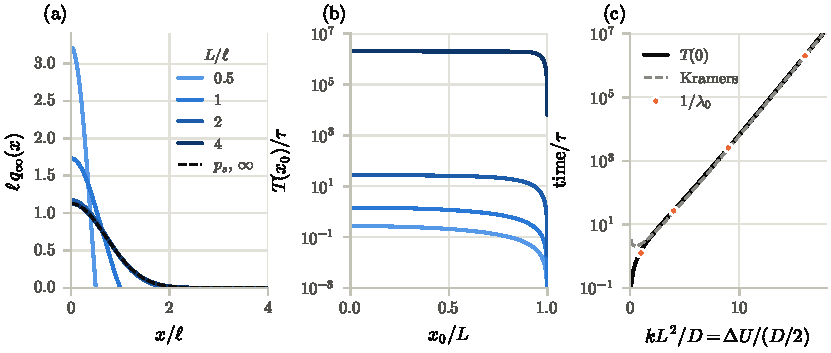
\includegraphics[width=\linewidth]{ou_mixed.pdf}
  \caption{Escape from a harmonic well: reflecting at the bottom, absorbing at $L$.
  (a)~Quasi-stationary densities; dashed, the half-Gaussian.
  (b)~Mean exit time (log scale); colours as in (a).
  (c)~Arrhenius plot: $T(0)$ and $1/\lambda_0$ against the barrier $\Delta U/(D/2)=L^2/\ell^2$, with the
  leading Kramers asymptote.}
  \label{fig:ou-mixed}
\end{figure}

% ==============================================================================
\section{Ornstein--Uhlenbeck on the circle}
\label{sec:ou-circle}

$A=-kx$ is not a function on a circle, so OU cannot simply be put on one. The nearest thing is to repeat it:
measure $x$ from the bottom of the well, take $A=-kx$ for $|x|<L/2$, and repeat with period $L$. This is a
sawtooth. At the antipode $x=\pm L/2$ the drift jumps from $-kL/2$ to $+kL/2$, pointing away on both sides, and
the potential $U=\tfrac12kx^2$ has a cusp. That point is special, but not because of the topology: $A$ is
discontinuous there, and \G{5.2.15}--\G{5.2.16} hold there as they would at a discontinuity anywhere. Cut at the
antipode, this is OU on $(-L/2,L/2)$ with Gardiner's periodic conditions but \emph{without} \G{5.2.19}; cut
anywhere else, it is a drift with an interior jump, and \G{5.2.19} holds. It is one problem either way.

\begin{keyresults}
$A=-kx$ for $|x|<L/2$, repeated with period $L$ (sawtooth); $B=D$; $\ell=\sqrt{D/k}$, $\tau=1/k$ as in
\cref{eq:ou-scales}. The cusp at $x=\pm L/2$ is the only special point.
\begin{align}
  p_s(x) &= \frac{e^{-x^2/\ell^2}}{\ell\sqrt\pi\operatorname{erf}(L/2\ell)}\quad(|x|\le L/2),\qquad
  J_s=0\ \ (\Phi=0) \\
  p(x,t\given x_0,0) &= \tfrac12\bigl[p_{\rm R}(|x|,t\given|x_0|)+\operatorname{sgn}(xx_0)\,
  p_{\rm A}(|x|,t\given|x_0|)\bigr] \\
  \text{spectrum} &= \{\nu^{\rm R}_nk\}\cup\{\nu^{\rm A}_nk\},\qquad \nu^{\rm R}_{n+1}=\nu^{\rm A}_n+1\ \text{exactly} \\
  Q_n &= Q^{\rm R}_n(|x|)\ \text{or}\ \operatorname{sgn}(x)\,Q^{\rm A}_n(|x|),\qquad
  P_n=p_sQ_n=\tfrac12P^{\rm R}_n(|x|)\ \text{or}\ \tfrac12\operatorname{sgn}(x)\,P^{\rm A}_n(|x|) \\
  D_{\rm eff} &= \frac{D\,(L/\ell)^2}{\pi\operatorname{erf}(L/2\ell)\operatorname{erfi}(L/2\ell)}
  \;\to\;\begin{cases}D, & L\ll\ell\\[2pt] \tfrac12L^2\lambda_0^{\rm mix}, & L\gg\ell\end{cases}
\end{align}
Here $p_{\rm R}$, $p_{\rm A}$, $\nu^{\rm R}_n$, $\nu^{\rm A}_n$ and $P^{\rm R,A}_n$, $Q^{\rm R,A}_n$ are the
propagators, eigenvalues and eigenfunctions of \cref{sec:ou-reflecting,sec:ou-absorbing} on $(0,L/2)$, and
$\lambda_0^{\rm mix}$ is the escape rate of
\cref{sec:ou-mixed} with its absorbing wall at the cusp, $L\to L/2$.
\end{keyresults}

\paragraph{Physical picture.} A periodic row of identical parabolic traps that touch at sharp ridges, such as a
one-dimensional lattice of optical traps with no gaps between them. The circle is one lattice cell, and winding
is hopping from trap to trap.

\paragraph{From Gardiner.} The cusp is a discontinuity in the sense of \Gs{5.2.1c}: $p$ and $J$ are continuous
there \G{5.2.15}--\G{5.2.16}, while ``the derivatives of $p$ are not necessarily continuous'', and here
$\partial_xp$ does jump. Since $\Phi=0$, $p_s$ is the potential solution \G{5.2.39}. The two sectors are the
Kummer problems of \cref{sec:ou-reflecting,sec:ou-absorbing}, that is, \G{5.2.116}--\G{5.2.117} with walls.
$D_{\rm eff}$ is \G{5.2.160} applied on the cover, as shown below.

\subsection{Folding into two intervals}

$A$ is odd under $x\to-x$, which fixes the bottom and the cusp. By \cref{sec:circle-toolkit} the even sector is
OU with reflecting walls at the bottom and at $L/2$, which is \cref{sec:ou-reflecting} with $L\to L/2$, and the
odd sector is \cref{sec:ou-absorbing} with $L\to L/2$. Gluing the two gives the propagator in the box. The
script checks that the glued density solves the equation, stays normalised, and has continuous $J$ at the
cusp; its slope jumps there (\cref{fig:ou-circle}a). The eigenfunctions glue the same way: the circle's $p_s$ is
half the interval's, so the interval's $Q_n$, extended evenly or oddly, keep $\int p_sQ_n^2=1$ over the whole
circle, and the $P_n$ are halved. At the cusp $Q_n$ and $Q_n'$ are continuous (the wall conditions $Q'=0$ and
$Q=0$ hold from both sides), and only $Q_n''$ jumps, with $A$. $P_n$ inherits the kink of $p_s$, while $P_n$ and
$J(P_n)$ stay continuous, as \G{5.2.15}--\G{5.2.16} require.

The ladder of \cref{sec:ou-map} then fixes the whole spectrum. Each reflecting level is an absorbing one plus
exactly $k$, so each doublet of the free circle (\cref{sec:circle}), where $\cos$ and $\sin$ had equal rates,
is split by exactly $k$, at every $L$ (\cref{fig:ou-circle}b):
\begin{itemize}
  \item for $L\ll\ell$ both members sit near the free doublet $2\pi^2n^2D/L^2$;
  \item for $L\gg\ell$ the pairs tend to $(1,2)k$, $(3,4)k$, \dots: the odd and even Hermite levels of
        \cref{sec:ou-hl-absorbing,sec:ou-hl-reflecting}, which together make the OU ladder $nk$ of
        \cref{sec:ou-line}, each level once.
\end{itemize}
In the symmetrised form of \cref{sec:operator}, the jump of $A$ by $kL$ at the cusp puts a repulsive
$\tfrac12kL\,\delta$ into $V$ on top of the harmonic well (\cref{fig:operators}c). Unlike the smooth barrier top
of \cref{sec:cos-circle}, it supports no levels of its own, which is why the levels here are single.

\subsection{Winding over the cusp}

\G{5.2.160} on the cover gives $D_{\rm eff}$ for any potential symmetric about the start. The first full
winding from the bottom is the exit from $(-L,L)$. By symmetry this is the interval $(0,L)$, reflecting at $0$
and absorbing at $L$, so with $\psi=e^{-2U/D}$
\begin{equation}
  T_{\rm w}=\frac2D\int_0^L\dd y\,e^{2U(y)/D}\int_0^y\dd z\,e^{-2U(z)/D}
  =\frac{L^2}{D}\,\avg{e^{2U/D}}\avg{e^{-2U/D}},
\end{equation}
where $\avg\cdot$ averages over one period. The second form uses $U(L-y)=U(y)$: substituting $y\to L-y$ turns
the inner integral into the rest of the period, so the double integral is half the product of the single ones.
With $D_{\rm eff}=L^2/T_{\rm w}$ (\cref{sec:circle-toolkit}) this is the Lifson--Jackson formula~\cite{lifson},
\begin{equation}
  D_{\rm eff}=\frac{D}{\avg{e^{2U/D}}\avg{e^{-2U/D}}}.
  \label{eq:lifson}
\end{equation}
For the sawtooth the two averages are $\ell\sqrt\pi\operatorname{erfi}(L/2\ell)/L$ and
$\ell\sqrt\pi\operatorname{erf}(L/2\ell)/L$, which gives the box.
\begin{itemize}
  \item For $L\ll\ell$ the well hardly matters and $D_{\rm eff}\to D$ (\cref{sec:circle}).
  \item For $L\gg\ell$ the particle hops between copies of the well. To get over, it must reach the cusp,
        which happens at the rate $\lambda_0^{\rm mix}$ of \cref{sec:ou-mixed} with the absorbing wall at $L/2$;
        from the cusp it falls either way with probability $\tfrac12$. So it hops to each neighbour at rate
        $\lambda_0^{\rm mix}/4$, and a random walk with steps $\pm L$ at total rate $\lambda_0^{\rm mix}/2$ has
        $D_{\rm eff}=\tfrac12L^2\lambda_0^{\rm mix}$. At $L=8\ell$ this matches \cref{eq:lifson} to
        $2\times10^{-6}$ (\cref{fig:ou-circle}c).
  \item $T_{\rm w}$ is the same from every starting point, not just the bottom; the script checks this from
        \G{5.2.158}. For winding, no point of the circle is special, not even the cusp.
\end{itemize}

\begin{figure}[tbp]
  \centering
  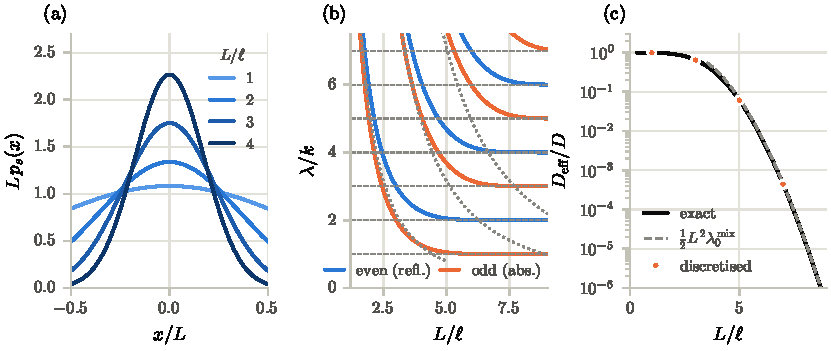
\includegraphics[width=\linewidth]{ou_circle.pdf}
  \caption{OU on the circle (sawtooth drift), $x$ measured from the bottom of the well.
  (a)~Stationary densities: truncated Gaussians, repeated, with a kink at the cusp $x=\pm L/2$.
  (b)~Spectrum: even sector (blue; reflecting walls at the bottom and the cusp) and odd sector (orange;
  absorbing). Each pair is split by exactly $k$. Dotted, the free doublets $2\pi^2n^2D/L^2$; dashed, the OU
  ladder.
  (c)~Effective diffusion of the lift: \cref{eq:lifson} (black), the hopping limit
  $\tfrac12L^2\lambda_0^{\rm mix}$ with the leading Kramers rate of \cref{sec:ou-mixed} (dashed), and an
  independent discretised computation (dots).}
  \label{fig:ou-circle}
\end{figure}

% ==============================================================================
\section{A smooth well on the circle}
\label{sec:cos-circle}

The cusp disappears if the harmonic well is replaced by the smooth periodic potential with the same curvature
at the bottom, $U=-kR^2\cos(x/R)$ with $R=L/2\pi$. Its drift $A=-kR\sin(x/R)$ is OU near the bottom, has a
smooth barrier top at the antipode, and has no special point at all. Adding a constant drift $v$ tilts the
potential and makes $\Phi=2vL/D\neq0$. That gives the one example in these notes of a NESS whose density is
not uniform. The model is the overdamped pendulum, or Adler's equation, with noise; Risken~\cite{risken}
(ch.~11) treats it in detail.

\begin{keyresults}
$A=v-kR\sin(x/R)$, $B=D$, $R=L/2\pi$. Two numbers set everything: the depth $\kappa=2R^2/\ell^2=(L/\ell)^2/2\pi^2$,
so that the barrier is $\Delta U/(D/2)=2\kappa$, and the tilt $v/kR$.
\begin{align}
  v=0:\quad p_s &= \frac{e^{\kappa\cos(x/R)}}{L\,I_0(\kappa)}\ \text{(von Mises)},\qquad J_s=0 \\
  \text{spectrum} &: \text{exact doublets};\qquad \lambda\to\frac{m^2k}{\kappa}\ (\kappa\ll1),\qquad
  \lambda\to nk\ (\kappa\gg1) \\
  P_\lambda,\ Q_\lambda &: \text{right, left eigenvectors of \cref{eq:cos-recurrence}};\quad
  v=0:\ P_\lambda=p_sQ_\lambda \\
  D_{\rm eff} &= \frac{D}{I_0(\kappa)^2}\;\simeq\;\frac{kL^2}{\pi}\,e^{-2\kappa}\quad
  \text{(Kramers, \G{5.2.174})} \\
  v\neq0:\quad & p_s,\ J_s\ \text{from \cref{eq:circle-ps}},\qquad v_{\rm w}=LJ_s\simeq\frac{D_{\rm eff}}{D}\,v\ \
  (v\to0) \\
  \kappa\to\infty:\quad v_{\rm w} &\to 0\ \ (|v|<kR),\qquad v_{\rm w}\to\operatorname{sgn}(v)\sqrt{v^2-k^2R^2}\ \ (|v|>kR)
\end{align}
\end{keyresults}

\paragraph{Physical picture.} $\mathcal U=-\mathcal U_0\cos(x/R)-Fx$, with $\kappa=\mathcal U_0/k_BT$.
\begin{itemize}
  \item Without tilt: a planar dipole in a field, whose orientation follows the von Mises (Langevin--Debye)
        distribution, or an overdamped pendulum.
  \item With tilt, the tilted washboard: a Josephson junction in the overdamped (RSJ) limit, where $x/R$ is the
        phase difference, the tilt is the bias current, and the winding velocity $v_{\rm w}$ is the dc voltage.
        \Cref{fig:cos-circle}c is then the noisy current--voltage curve of Ambegaokar and Halperin~\cite{ambegaokar}.
  \item Colloids driven around a corrugated ring trap realise it directly, including the giant diffusion near
        threshold~\cite{leegrier} and the breakdown of the equilibrium Einstein relation~\cite{blickle}.
\end{itemize}

\paragraph{From Gardiner.} With $v=0$, $\Phi=0$ and \G{5.2.39} gives the von Mises density. The eigenfunctions
obey \Gs{5.2.5} with periodic $Q$, but the equation is no longer Hermite's or Kummer's; a Fourier series turns
it into a three-term recurrence instead. $D_{\rm eff}$ is \G{5.2.160} on the cover, exactly as in
\cref{sec:ou-circle}, and its large-$\kappa$ limit is Gardiner's Kramers formula \G{5.2.174}. With $v\neq0$,
$p_s$ and $J_s$ are \G{5.2.47} and the corrected \G{5.2.46}, or \cref{eq:circle-ps}.

\subsection{No special point}

$A$ is smooth and, without tilt, odd under $x\to-x$. So the circle folds into the cosine well on $(0,L/2)$, with
walls at the bottom and at the barrier top, reflecting (even sector) or absorbing (odd sector). Now
$A'=-k\cos(x/R)$ is not constant, and the ladder of \cref{sec:ou-map} does not apply. In Fourier space, with
$p=\sum_mc_me^{imx/R}$,
\begin{equation}
  \dot c_m=-\Bigl(\frac{Dm^2}{2R^2}+\frac{ivm}{R}\Bigr)c_m+\frac{km}2\,(c_{m-1}-c_{m+1}),
  \label{eq:cos-recurrence}
\end{equation}
a three-term recurrence whose truncations converge like Bessel functions. The script solves it, and checks it
against an independent discretisation. Its eigenvectors $c^{(\lambda)}$ are Gardiner's
$P_\lambda=\sum_mc^{(\lambda)}_me^{imx/R}$. Writing $Q_\lambda=\sum_mb^{(\lambda)}_me^{-imx/R}$ turns the pairing
\G{5.2.79} into $2\pi R\sum_mb^{(\lambda)}_mc^{(\lambda')}_m$, so the $b^{(\lambda)}$ are the left eigenvectors of
the same matrix, normalised against the right ones. Without tilt $P_\lambda=p_sQ_\lambda$, and each doublet has one
even $Q_\lambda$ (a cosine series, the reflecting sector of the fold) and one odd (a sine series, the absorbing
sector). With tilt $J_s\neq0$ and $P_\lambda\neq p_sQ_\lambda$: the script checks that $P_\lambda/p_s$ then fails the
backward equation, while the left eigenvectors satisfy it.

\subsection{Exact doublets}

Every nonzero level of the cosine well is exactly doubly degenerate, for every $\kappa$
(\cref{fig:cos-circle}b), so the reflecting and absorbing intervals of the fold have identical nonzero spectra.
The reason is visible in \cref{eq:cos-recurrence}. A mode with $\lambda\neq0$ must have $c_0=0$, because $c_0$
is the total probability, which does not decay. With $c_0=0$ the equations for $m>0$ and for $m<0$ no longer
talk to each other, and the two chains are mirror images. (A $\cos(2x/R)$ term in $U$ would couple $m=\pm1$
directly and split the doublets.)

In a deep well the two members of a doublet have different physics. For $\kappa\gg1$ the levels tend to $nk$,
$n\ge1$, each twice. One copy is the OU ladder at the bottom of the well (\cref{sec:ou-line}). The other lives at
the barrier top, where a density relaxes by sliding off the hilltop, also at rates $k,2k,\dots$, because the
curvature there is $-k$. In the symmetrised form of \cref{sec:operator} these are the levels of the two wells
of $V$, at the bottom and at the top of $U$ (\cref{fig:operators}b). Compare \cref{sec:ou-circle}: a cusp sheds probability at once, has no ladder of its
own, and leaves the levels single. For $\kappa\ll1$ the levels tend to the free doublets
$m^2k/\kappa=Dm^2/2R^2$ of \cref{sec:circle}.

\subsection{Winding: Kramers with a smooth barrier}

\Cref{eq:lifson} with $\avg{e^{\pm\kappa\cos(x/R)}}=I_0(\kappa)$ gives $D_{\rm eff}=D/I_0(\kappa)^2$ exactly. For a
deep well this is hopping over a smooth barrier, the case Gardiner treats in \Gs{5.2.7c}. With his $D$ replaced
by our $D/2$, and $U''=k$ at the bottom and $-k$ at the top, \G{5.2.174} gives $2\pi\tau e^{2\kappa}$ for the
time to cross in one direction. On the circle the barrier can be crossed either way, so
$T_{\rm w}\simeq\pi\tau e^{2\kappa}$ and $D_{\rm eff}=L^2/T_{\rm w}\simeq(kL^2/\pi)e^{-2\kappa}$. This is the
leading term of $D/I_0(\kappa)^2$; the next is a factor $1-1/4\kappa$. Unlike \cref{sec:ou-mixed}, where the
barrier top is a wall, and \cref{sec:ou-circle}, where it is a cusp, Gardiner's prefactor applies here
unchanged.

\subsection{Tilt: a current, depinning, giant diffusion}

With $v\neq0$, $\Phi=2vL/D\neq0$ and a current circulates (\cref{fig:cos-circle}a).
\begin{itemize}
  \item \textbf{Small tilt.} Expanding \cref{eq:circle-ps} to first order in $v$ gives
        $v_{\rm w}=v/\avg{e^{2U/D}}\avg{e^{-2U/D}}=v\,D_{\rm eff}/D$. The mobility of the winding equals its diffusion
        constant over $D$: the Einstein relation, which here combines the topology (the current) with
        Lifson--Jackson (the diffusion).
  \item \textbf{Depinning.} Without noise, $\dot x=v-kR\sin(x/R)$ has a fixed point while $|v|<kR$, and the
        rotor is locked. For $|v|>kR$ it runs, with period $\oint\dd x/(v-kR\sin(x/R))=L/\sqrt{v^2-k^2R^2}$.
        Noise smooths the transition: below threshold the rotor slips by thermally activated hops, and above
        it the flow is nearly deterministic (\cref{fig:cos-circle}c).
  \item \textbf{Giant diffusion.} Near threshold $D_{\rm eff}$ exceeds the bare $D$, by a factor that grows as
        the noise decreases~\cite{reimann} (\cref{fig:cos-circle}d). There, each revolution is a race between
        lingering near the almost-fixed point and running, so the time per revolution is broadly distributed,
        and that spreads the winding. The script computes $D_{\rm eff}=\Lambda''(0)$ from
        \cref{eq:cos-recurrence} with $\partial_x\to\partial_x-s$, and checks it against a discretisation and a
        simulation.
  \item The NESS density is not the Boltzmann factor of any potential. For large tilt it approaches the
        deterministic dwell-time density $p_s\propto1/|v-kR\sin(x/R)|$, highest where the rotor is slowest.
\end{itemize}

\begin{figure}[tbp]
  \centering
  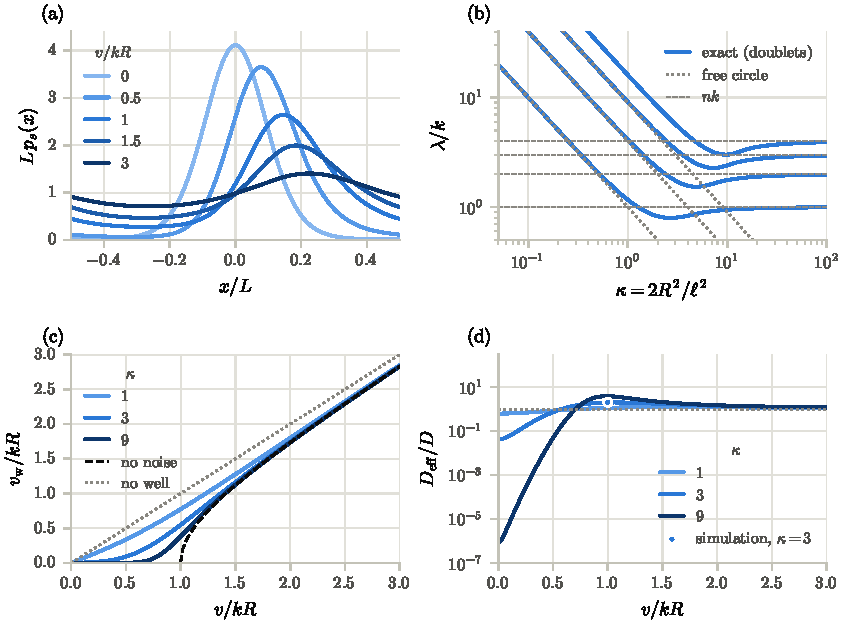
\includegraphics[width=\linewidth]{cos_circle.pdf}
  \caption{The cosine well on the circle, $x$ measured from the bottom.
  (a)~Stationary densities at $\kappa=3$ for several tilts: von Mises at $v=0$, a current-carrying NESS
  otherwise.
  (b)~Spectrum without tilt: every level is a doublet. Dotted, the free circle $m^2k/\kappa$; dashed, the OU
  ladder $nk$.
  (c)~Winding velocity against tilt for three depths; dashed, the noiseless rotor; dotted, no well.
  (d)~Effective diffusion of the lift; dotted, the bare $D$. The dot is a simulation of 4000 paths over
  $200\,\tau$.}
  \label{fig:cos-circle}
\end{figure}

% ==============================================================================
\section{Summary of Ornstein--Uhlenbeck}
\label{sec:ou-summary}

\begin{table}[h]
\centering
\small
\renewcommand{\arraystretch}{1.35}
\begin{tabular}{@{}l l l@{}}
\toprule
Walls (bottom of well at $0$) & Slowest rate & Long times \\
\midrule
none                     & gap $k$                         & $p_s=e^{-x^2/\ell^2}/\ell\sqrt\pi$ \\
reflecting at $0$        & gap $2k$                        & half-Gaussian \\
absorbing at $0$         & bottom $k$, gap $2k$            & QSDs for $\lambda\in(0,k]$; Rayleigh from point starts \\
reflecting $0$, $L$      & $\frac{\pi^2D}{2L^2}\to2k$      & truncated half-Gaussian \\
absorbing $0$, $L$       & $\frac{\pi^2D}{2L^2}\to k$      & QSD: sine $\to$ Rayleigh \\
refl.\ $0$, abs.\ $L$    & $\frac{\pi^2D}{8L^2}\to$ Kramers & $T\simeq\frac{\sqrt\pi\,\tau\ell}{2L}e^{L^2/\ell^2}$ \\
circle, sawtooth         & $\frac{2\pi^2D}{L^2}\to k$; pairs split by $k$ & cusp; $D_{\rm eff}\to\frac12L^2\lambda_0^{\rm mix}$ \\
circle, cosine well      & $\frac{k}{\kappa}\to k$; exact doublets & von Mises, $D_{\rm eff}=D/I_0(\kappa)^2$; tilt: NESS \\
\bottomrule
\end{tabular}
\caption{Ornstein--Uhlenbeck in every geometry; $\ell=\sqrt{D/k}$, $\tau=1/k$. Arrows go from $L\ll\ell$ to
$L\gg\ell$.}
\label{tab:ou-summary}
\end{table}

\begin{itemize}
  \item With walls at the bottom of the well, Gardiner's substitution $y=xe^{kt}$ turns every Part~I result
        into an OU result. Free spreading freezes into stationary and quasi-stationary states, and algebraic
        decay becomes exponential.
  \item With an absorbing wall at the bottom there is a continuum of QSDs, $\lambda\in(0,k]$. A start with a
        finite mean reaches the Rayleigh one; a power-law tail $x^{-1-\nu}$, $\nu<1$, reaches $q_\nu$.
  \item Walls at the bottom select from the Hermite ladder: even modes for reflecting, odd for absorbing.
        The nonzero reflecting levels are the absorbing ones shifted up by exactly $k$.
  \item On an interval, the length to compare with is $\ell$. For $L\ll\ell$ the results are those of Part~I;
        for $L\gg\ell$ they are the half-line results, or Kramers escape (\cref{fig:ou-summary}).
  \item Across the three parts, escape against a force costs $e^{2\Delta U/D}$: nothing for a flat potential
        ($T\sim L^2/D$), $e^{2L/\ell_v}$ for a linear one, and $e^{L^2/\ell^2}$ for a harmonic one.
  \item OU fits on a circle only with a special point, the cusp where the sawtooth drift jumps. Folding and the
        ladder then solve it with no new work, and every free doublet is split by exactly $k$. The smooth
        cosine well has no special point, and its doublets stay exactly degenerate.
  \item The prefactor of the escape rate depends on the shape of the barrier top: a wall
        (\cref{sec:ou-mixed}); a cusp, crossed with probability $\tfrac12$ once reached (\cref{sec:ou-circle});
        a smooth maximum, Gardiner's \G{5.2.174} (\cref{sec:cos-circle}).
\end{itemize}

\begin{figure}[tbp]
  \centering
  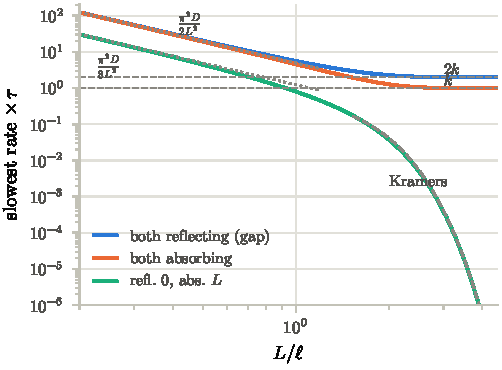
\includegraphics[width=0.6\linewidth]{ou_summary.pdf}
  \caption{Slowest rates of the three OU intervals against $L/\ell$, with their Part~I asymptotes (dotted),
  half-line limits (dashed horizontal) and the Kramers rate (dashed).}
  \label{fig:ou-summary}
\end{figure}

% ==============================================================================
\part{More exactly solvable potentials}
\label{part:solvable}

Parts I--III are the free particle, the linear potential and the harmonic potential. One mechanism explains why
they are solvable, and it also identifies the other solvable potentials: the factorisation of the symmetrised
operator (\cref{sec:solvable}). Three worked sections follow, each chosen to connect back to Parts I--III: the
logarithmic potential, which is radial motion in $d$ dimensions (\cref{sec:radial}); a soft V-shaped potential
(\cref{sec:lncosh}); and a well that builds its own walls (\cref{sec:lncos}). Throughout, $A=-U'$ and $B=D$, so
$p_s\propto e^{-2U/D}$ and the symmetrised potential \cref{eq:schrodinger} is $V=U'^2/2D-U''/2$.

\section{Factorisation, partners and shape invariance}
\label{sec:solvable}

\paragraph{From Gardiner.} Not in the book. The section builds on the symmetrised form of
\cref{sec:operator}, that is, on Gardiner's $p=p_sq$ \G{5.2.71}, and on the ladder of \cref{sec:ou-map}.

\paragraph{Factorisation.} With $B=D$ the Schr\"odinger operator \cref{eq:schrodinger} factorises, as
multiplying out shows:
\begin{equation}
  H=\mathcal A^\dagger\mathcal A,\qquad \mathcal A=\sqrt{\tfrac D2}\Bigl(\partial_x-\frac AD\Bigr),\qquad
  \mathcal A^\dagger=\sqrt{\tfrac D2}\Bigl(-\partial_x-\frac AD\Bigr).
  \label{eq:factor}
\end{equation}
Since $\partial_x\sqrt{p_s}=(A/D)\sqrt{p_s}$, $\mathcal A\sqrt{p_s}=0$: the ground state at $\lambda=0$. And
$\int\psi H\psi=\int(\mathcal A\psi)^2\ge0$, which is the Dirichlet form \cref{eq:dirichlet} again.

\paragraph{The partner is the inverted potential.} Reversing the order gives
\begin{equation}
  \tilde H=\mathcal A\mathcal A^\dagger=-\tfrac12D\,\partial_x^2+\tilde V,\qquad
  \tilde V=\frac{A^2}{2D}-\frac{A'}{2},
  \label{eq:partner}
\end{equation}
the Schr\"odinger operator of the drift $-A$, that is, of the inverted potential $-U$. The two are intertwined,
$\mathcal AH=\tilde H\mathcal A$. So $\mathcal A$ carries every eigenfunction of $H$ with $\lambda\neq0$ to one of
$\tilde H$ with the same $\lambda$, and $\mathcal A^\dagger$ carries it back. In Fokker--Planck terms, with
$\psi=\sqrt{p_s}\,Q$, one has $\mathcal A\psi=\sqrt{D/2}\,\sqrt{p_s}\,Q'$: \emph{the derivative of a backward
eigenfunction is, up to the weight, an eigenfunction of the inverted problem, with the same rate.} A potential
and its inverse therefore share every nonzero rate, as long as the wall conditions match.
\begin{itemize}
  \item This is the ladder of \cref{sec:ou-map} in general form. For OU the inverted potential gives
        $\tilde V=V+k$, so $Q'$ is again an OU eigenfunction, with the rate lowered by $k$.
  \item It is also the origin of the exact doublets of \cref{sec:cos-circle}. There $-U$ is $U$ rotated by half
        a turn $S$, so $S\mathcal AS=-\mathcal A^\dagger$, and $S\mathcal A$ commutes with $H$ while squaring to
        $-H$. On a real eigenfunction with $\lambda>0$ it cannot act as a number, since that number would square
        to $-\lambda$. So every nonzero level has at least two eigenfunctions.
\end{itemize}

\paragraph{Shape invariance.} Sometimes the partner belongs to the same family: $\tilde V(x;s)=V(x;s')+R(s)$, with a
shifted parameter $s'$ and a constant $R$. Then the ground state of the partner, at $R(s)$, is the first excited
state of the original problem, and repeating the step gives the whole spectrum by algebra:
\begin{equation}
  \lambda_n(s)=R(s_0)+R(s_1)+\dots+R(s_{n-1}),\qquad s_0=s,\quad s_{j+1}=s_j' .
  \label{eq:shape}
\end{equation}
The eigenfunctions follow by repeated $\mathcal A^\dagger$, which is where the Rodrigues formulas of the classical
polynomials come from. The ladder stops when the partner's ground state stops being normalisable; that is where
a finite set of discrete levels ends and a continuum begins. The script checks each of these partner identities:
\begin{itemize}
  \item OU: $s'=s$, $R=k$, so $\lambda_n=nk$ (Part~III).
  \item Harmonic plus logarithmic: $c\to c+D$, which raises the dimension $d$ by two, and $R=2k$, so
        $\lambda_n=2nk$ (\cref{sec:radial}).
  \item $a\ln\cosh(x/w)$: $s\to s-1$, $R=(D/2w^2)(2s-1)$, so $\lambda_n=(D/2w^2)\,n(2s-n)$ for $n<s$
        (\cref{sec:lncosh}).
  \item $-a\ln\cos(x/w)$: $s\to s+1$, $R=(D/2w^2)(2s+1)$, so $\lambda_n=(D/2w^2)\,n(n+2s)$ (\cref{sec:lncos}).
  \item Free motion and constant drift: $\tilde V=V$ and $R=0$. There is no ladder, and the spectrum is a
        continuum.
\end{itemize}

\paragraph{The solvable potentials.} \Cref{tab:solvable} lists the shape-invariant potentials of supersymmetric
quantum mechanics~\cite{cooper}, rewritten as Fokker--Planck potentials (\cref{fig:solvable}). Two of them are
not worked out in these notes, but their spectra are checked numerically.
\begin{itemize}
  \item The linear-plus-logarithmic potential is a hydrogen atom in disguise: infinitely many discrete rates
        accumulate at the continuum edge $v^2/2D$, and $p_s$ is a gamma distribution. Physically it is the
        distance from the origin of a particle in $d$ dimensions pulled toward it by a force of constant magnitude;
        the logarithm is the entropic term of \cref{sec:radial}.
  \item The Morse potential is a soft exponential wall with gravity, the soft version of
        \cref{sec:drift-hl-reflecting}. Physically it is a colloid hovering above a like-charged surface: screened
        electrostatic repulsion holds it up and gravity pulls it down. Total internal reflection microscopy
        measures exactly this potential~\cite{prieve}.
\end{itemize}
The cosine well on a circle (\cref{sec:cos-circle}) is not shape-invariant: its symmetrised potential has two
cosine harmonics, which is why it needs a recurrence instead.

\begin{table}[h]
\centering
\footnotesize
\renewcommand{\arraystretch}{1.45}
\setlength{\tabcolsep}{4pt}
\begin{tabular}{@{}l l l l l@{}}
\toprule
$U(x)$ & Domain & $p_s$ & $\lambda_n$ & Section \\
\midrule
$0$ & line & --- & continuum from $0$ & \ref{sec:line} \\
$vx$ & $x>0$, reflecting & $e^{-2vx/D}$ & $0$; continuum from $v^2/2D$ & \ref{sec:drift-hl-reflecting} \\
$\tfrac12kx^2$ & line & $e^{-kx^2/D}$ & $nk$ (Hermite) & \ref{sec:ou-line} \\
$\tfrac12kx^2-c\ln x$ & $x>0$ & $x^{2c/D}e^{-kx^2/D}$ & $2nk$ (Laguerre) & \ref{sec:radial} \\
$vx-c\ln x$ & $x>0$ & $x^{2c/D}e^{-2vx/D}$ & $\frac{v^2}{2D}\bigl[1-\frac{\sigma^2}{(n+\sigma)^2}\bigr]$, $\sigma=\frac cD$ (Laguerre) & --- \\
$vx+U_0e^{-x/w}$ & line & $e^{-2vx/D-(2U_0/D)e^{-x/w}}$ & $\frac{D}{2w^2}n(2s-n)$, $n<s=\frac{vw}D$ (Laguerre) & --- \\
$a\ln\cosh(x/w)$ & line & $\operatorname{sech}^{2s}(x/w)$ & $\frac{D}{2w^2}n(2s-n)$, $n<s=\frac aD$ (Jacobi) & \ref{sec:lncosh} \\
$-a\ln\cos(x/w)$ & $|x|<\frac{\pi w}2$ & $\cos^{2s}(x/w)$ & $\frac{D}{2w^2}n(n+2s)$ (Gegenbauer) & \ref{sec:lncos} \\
\bottomrule
\end{tabular}
\caption{Fokker--Planck potentials with exactly known spectra ($A=-U'$, $B=D$). Where a continuum exists it
starts at $v^2/2D$, the value of $V$ at infinity.}
\label{tab:solvable}
\end{table}

\begin{figure}[tbp]
  \centering
  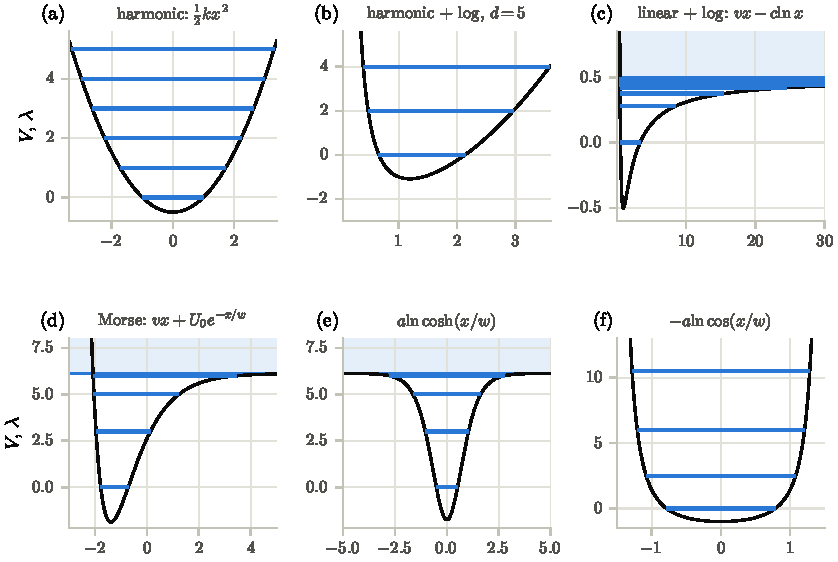
\includegraphics[width=\linewidth]{solvable.pdf}
  \caption{The solvable potentials of \cref{tab:solvable}, in the symmetrised picture: $V=U'^2/2D-U''/2$
  (black), the discrete rates drawn where $V<\lambda$ (blue), and the continuum (shaded) where there is one. $D=1$
  and (a) $k=1$; (b) $d=5$; (c) $v=1$, $\sigma=2$; (d) $s=3.5$, $w=U_0=1$; (e) $s=3.5$, $w=1$; (f) $s=2$, $w=1$.
  Discrete-only spectra (a, b, f) come from potentials that grow faster than linearly. The others level off at
  $V=v^2/2D$, with finitely many levels below it (d, e), or infinitely many crowding up to it (c).}
  \label{fig:solvable}
\end{figure}

% ==============================================================================
\section{Logarithmic potentials: radial motion in \texorpdfstring{$d$}{d} dimensions}
\label{sec:radial}

\begin{keyresults}
$U=-c\ln x$, optionally $+\tfrac12kx^2$, on $x>0$ with $B=D$. Write $c=(d-1)D/2$ and $\mu=d/2-1$. For integer $d$,
$x=r$ is the distance from the origin of a $d$-dimensional free ($k=0$) or OU motion; the formulas hold for every
real $d>0$. With $\ell=\sqrt{D/k}$, $m_t=r_0e^{-kt}$ and $\sigma_t^2=\tfrac12\ell^2(1-e^{-2kt})$:
\begin{align}
  k=0:\quad p(r,t\given r_0,0) &= \frac{r}{Dt}\Bigl(\frac{r}{r_0}\Bigr)^{\mu}e^{-(r^2+r_0^2)/2Dt}\,
  I_\mu\Bigl(\frac{rr_0}{Dt}\Bigr)\qquad\text{(Bessel process)} \\
  k>0:\quad p(r,t\given r_0,0) &= \frac{r}{\sigma_t^2}\Bigl(\frac{r}{m_t}\Bigr)^{\mu}e^{-(r^2+m_t^2)/2\sigma_t^2}\,
  I_\mu\Bigl(\frac{rm_t}{\sigma_t^2}\Bigr) \\
  p_s(r) &= \frac{2\,r^{d-1}e^{-r^2/\ell^2}}{\ell^d\,\Gamma(d/2)}\quad\text{(chi)} \\
  \lambda_n &= 2nk,\quad Q_n=\sqrt{\frac{n!\,\Gamma(d/2)}{\Gamma(n+d/2)}}\,L_n^{(\mu)}\bigl(r^2/\ell^2\bigr),
  \quad P_n=p_sQ_n \\
  k=0:\quad P_\lambda &= \frac{r^{\mu+1}}{\sqrt D}\,J_\mu\Bigl(r\sqrt{\tfrac{2\lambda}D}\Bigr),\quad
  Q_\lambda=\frac{r^{-\mu}}{\sqrt D}\,J_\mu\Bigl(r\sqrt{\tfrac{2\lambda}D}\Bigr),\quad \lambda>0 \\
  k=0:\quad \Pr(\text{ever reach }a<r_0) &= 1\ \ (d\le2),\qquad (a/r_0)^{d-2}\ \ (d>2)
\end{align}
For $d=1$, $2$ and $3$ these are \cref{sec:ou-hl-reflecting}, Gardiner's Rayleigh process, and $e^{kt}r/r_0$ times
\cref{sec:ou-hl-absorbing}. For $d\ge2$ the origin is never reached and needs no condition; for $d<2$ the box
assumes it reflects. Absorption at the origin, and $d\le0$, are in \cref{sec:sqrt}.
\end{keyresults}

\paragraph{Physical picture.} The distance from a fixed point of a particle diffusing in $d$ dimensions, freely or
in an isotropic trap. The logarithmic potential is entropic: $\mathcal U=-(d-1)k_BT\ln r$ is $-T$ times the
entropy $k_B\ln r^{d-1}$ of the sphere of radius $r$, so it pushes outward because there is more room further out.
\begin{itemize}
  \item With an absorbing sphere of radius $a$ in three dimensions, the reach probability $a/r_0$ underlies
        Smoluchowski's rate for diffusion-limited reactions.
  \item With a trap in two dimensions, $r$ is the amplitude of a noisy oscillator or optical field, Rayleigh
        distributed; this is Gardiner's motivation in \Gs{4.4.5}, for example a laser below threshold.
  \item The squared radius is the CIR or Feller process of interest-rate models and of populations with
        immigration.
\end{itemize}

\paragraph{From Gardiner.} \Gs{4.4.5} converts a pair of OU processes \G{4.4.32} to polar coordinates. Itô's
formula gives the amplitude equation \G{4.4.41b}, $\dd a=(-\gamma a+\varepsilon^2/2a)\,\dd t+\varepsilon\,\dd W_a$,
which is $d=2$ with $c=D/2$; the whole logarithmic potential is the Itô term. \Gs{5.2.6d} then solves this
Rayleigh process, \G{5.2.127}--\G{5.2.138}: $p_s$ is \G{5.2.129}, the eigenfunctions are Laguerre polynomials
\G{5.2.132}--\G{5.2.134} with $\lambda=2n\gamma$ \G{5.2.133}, and the propagator is the series \G{5.2.135}. His
$\gamma$ is our $k$ and his $\mu=\varepsilon^2/2$ is our $D/2$. General $d$ changes only the Laguerre index, to
$d/2-1$, and the normalisation: his $Q_\lambda=L_n(\gamma x^2/2\mu)$ \G{5.2.134} is already normalised for $d=2$, where
the factor in the box is $1$. The reach probability is the corrected splitting probability \G{5.2.190} with
$\psi=r^{2c/D}=r^{d-1}$.

\subsection{From the line, in \texorpdfstring{$d$}{d} dimensions}

The radius $r=|\mathbf x|$ of a $d$-dimensional Gaussian has as its density the Gaussian of \cref{sec:line} (or of
\cref{sec:ou-line}) integrated over the sphere of radius $r$. The angular integral is
$\int\dd\Omega\,e^{(rm/\sigma^2)\cos\theta}\propto(rm/\sigma^2)^{-\mu}I_\mu(rm/\sigma^2)$, which gives the box. The
Itô drift of $r$ is $(d-1)D/2r$: a repulsion from the origin by the potential $-c\ln r$. It is purely geometric:
in more than one dimension there are more directions leading away from the origin than toward it.
\begin{itemize}
  \item $d=1$: $I_{-1/2}$ is a $\cosh$, and the box is the image pair of
        \cref{sec:hl-reflecting,sec:ou-hl-reflecting}. The origin acts as a mirror.
  \item $d=3$: $I_{1/2}$ is a $\sinh$, and the box is $e^{kt}r/r_0$ times the absorbing image pair of
        \cref{sec:hl-absorbing,sec:ou-hl-absorbing}. That is the Doob transform with $h=x$. Radial motion in three
        dimensions is one-dimensional motion conditioned never to reach the origin, as anticipated in
        \cref{sec:hl-absorbing}. With OU, the conditioned process of \cref{sec:ou-hl-absorbing} has stationary
        density $\propto x^2e^{-x^2/\ell^2}$, the chi density with $d=3$.
  \item $d=2$: Gardiner's Rayleigh process. Its $p_s=(2r/\ell^2)e^{-r^2/\ell^2}$ is the same Rayleigh density that
        is the QSD of \cref{sec:ou-hl-absorbing}.
  \item The origin: for $d\ge2$ ($c\ge D/2$) the repulsion is strong enough that the origin is never reached. In
        Feller's classification \Gs{5.2.1e} it is an entrance boundary, so the potential supplies the wall
        condition and none may be imposed. For $0<d<2$ the origin is reached and a condition has to be chosen; for
        $d\le0$ the logarithm attracts and the origin is an exit (\cref{sec:sqrt}).
\end{itemize}

\subsection{Spectrum and recurrence}

\begin{itemize}
  \item By shape invariance (\cref{sec:solvable}) the partner in dimension $d$ is the problem in dimension $d+2$,
        shifted by $2k$. So $\lambda_n=2nk$ in every dimension: the even OU levels of \cref{sec:ou-hl-reflecting}.
        Only the eigenfunctions, the Laguerre polynomials $L_n^{(\mu)}$, know $d$.
  \item For $k=0$ the spectrum is a continuum from $0$, as on the line. Its eigenfunctions are Bessel functions,
        $P_\lambda$ and $Q_\lambda$ of the box, normalised to $\delta(\lambda-\lambda')$ with the weight
        $p_s=r^{d-1}$; integrating $P_\lambda(r)Q_\lambda(r_0)e^{-\lambda t}$ over $\lambda$ (Weber's integral) gives
        the Bessel-process propagator. For $d=1$ they are the cosines of \cref{sec:hl-reflecting}, for $d=3$ the
        sines of \cref{sec:hl-absorbing} times $r$ (forward) or $1/r$ (backward), the Doob transform with $h=r$.
        Whether the particle comes back is
        decided by the splitting probability (\cref{sec:fpt-toolkit}) with $\psi=r^{d-1}$:
        $\Pr(\text{reach }a\text{ before }R)=\int_{r_0}^Ry^{1-d}\dd y\big/\int_a^Ry^{1-d}\dd y$. As $R\to\infty$
        this tends to $1$ for $d\le2$ and to $(a/r_0)^{d-2}$ for $d>2$ (\cref{fig:radial}c). Brownian motion is
        recurrent in one and two dimensions and transient in more (P\'olya). In this language, recurrence holds
        exactly when the logarithmic repulsion is $c\le D/2$.
  \item The squared radius $y=r^2$ obeys $\dd y=(dD-2ky)\,\dd t+2\sqrt{Dy}\,\dd W$ by Itô's formula. That is the
        Cox--Ingersoll--Ross, or Feller, process of interest-rate and population models, with the same
        spectrum $2nk$.
\end{itemize}

\begin{figure}[tbp]
  \centering
  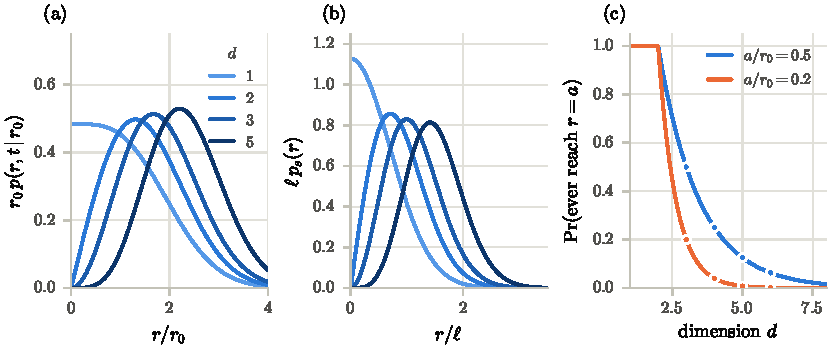
\includegraphics[width=\linewidth]{radial.pdf}
  \caption{Radial motion; colours give the dimension $d$ in (a) and (b).
  (a)~Free motion (Bessel process) from $r_0$ at $Dt=r_0^2$. The repulsion $(d-1)D/2r$ empties the region near
  the origin.
  (b)~Stationary chi densities of the radius of a $d$-dimensional OU motion; $d=2$ is the Rayleigh density.
  (c)~Probability that free motion ever comes within $a$ of the origin. Curves are $(a/r_0)^{d-2}$; dots are the
  splitting-probability quadrature.}
  \label{fig:radial}
\end{figure}

% ==============================================================================
\section{A soft V: \texorpdfstring{$U=a\ln\cosh(x/w)$}{U = a ln cosh(x/w)}}
\label{sec:lncosh}

\begin{keyresults}
$A=-v\tanh(x/w)$ with $v=a/w$, $B=D$, on the line. For $|x|\gg w$ the potential is linear, $U\approx v|x|$; for
$|x|\ll w$ it is harmonic, $U\approx\tfrac12kx^2$ with $k=a/w^2$. The drift scales are those of Part~II,
$\ell=D/v$ and $\tau=D/v^2$, and the shape is set by $s=a/D=w/\ell$.
\begin{align}
  p_s(x) &= \frac{\Gamma(s+\frac12)}{\sqrt\pi\,\Gamma(s)\,w}\operatorname{sech}^{2s}(x/w) \\
  V &= \frac1{2\tau}-\frac{D}{2w^2}\,\frac{s(s+1)}{\cosh^2(x/w)}\quad\text{(P\"oschl--Teller)} \\
  \lambda_n &= \frac{D}{2w^2}\,n(2s-n),\quad n=0,1,\dots,\ n<s;\qquad\text{continuum from }\frac1{2\tau} \\
  Q_n &\propto \cosh^n(x/w)\,P_n^{(s-n,\,s-n)}\bigl(\tanh(x/w)\bigr)\quad\text{(Jacobi)} \\
  P_n &= p_sQ_n\propto\operatorname{sech}^{2s-n}(x/w)\,P_n^{(s-n,\,s-n)}\bigl(\tanh(x/w)\bigr) \\
  s\to0\ (v\text{ fixed})&:\ U\to v|x|,\ \text{only }\lambda_0;\qquad s\to\infty\ (k\text{ fixed}):\ \lambda_n\to nk
\end{align}
$P_n^{(a,b)}$ is the Jacobi polynomial, not one of Gardiner's $P_\lambda$; each $Q_n$ is normalised by $\int p_sQ_n^2=1$.
\end{keyresults}

\paragraph{Physical picture.} $\mathcal U=2sk_BT\ln\cosh(x/w)$: a restoring force that is linear near the centre
and saturates at the magnitude $F=\gamma v$ far away. One example is a bead sliding under gravity in a V-shaped
groove with a rounded bottom of width $w$. Another is a feedback trap that caps its restoring force.

\paragraph{From Gardiner.} $p_s$ is \G{5.2.39}; the rest is not in the book. First-passage quantities are the
quadratures of \cref{sec:fpt-toolkit}, as for any potential (\cref{sec:general}).

\subsection{Between a V and a parabola}

\begin{itemize}
  \item Both limits are earlier sections. As $s\to0$ at fixed $v$, $U\to v|x|$: the drift toward a reflecting wall of
        \cref{sec:drift-hl-reflecting}, unfolded at the wall. It has the stationary density $e^{-2|x|/\ell}/\ell$,
        a single level at $0$, and a continuum from $1/2\tau$. As $s\to\infty$ at fixed curvature $k$ the problem
        becomes OU (\cref{sec:ou-line}); exactly, $\lambda_1=k(1-1/2s)$.
  \item In between, $p_s$ has a Gaussian core of width $\sqrt{D/k}=\ell\sqrt s$ and exponential tails
        $e^{-2|x|/\ell}$ (\cref{fig:lncosh}a).
  \item The continuum starts at $V(\infty)=1/2\tau$, by the rule of \cref{sec:operator}. Below it there are
        $\lceil s\rceil$ discrete levels, and a new one detaches from the edge each time $s$ passes an integer
        (\cref{fig:lncosh}b). In Schr\"odinger language these are the bound states of the P\"oschl--Teller well.
        Here they follow from the ladder of \cref{sec:solvable}, which stops once $s-n<0$. In Gardiner's terms,
        $P_n\sim e^{-(2s-n)|x|/w}$ and $Q_n\sim e^{n|x|/w}$, so $\int P_nQ_n$ \G{5.2.79} converges exactly when $n<s$.
  \item Above the edge, $P_\lambda$ and $Q_\lambda$ are scattering states. Far from the centre they are the gauge
        modes of Part~II on each side, $P_\lambda\propto e^{-|x|/\ell}\cos(k|x|+\delta_k)$ and
        $Q_\lambda\propto e^{|x|/\ell}\cos(k|x|+\delta_k)$, with $\lambda=1/2\tau+\tfrac12Dk^2$.
  \item Relaxation: for $s>1$ the slowest rate is the discrete $\lambda_1<1/2\tau$, approached exponentially, as in
        OU. For $s\le1$ there is no level between $0$ and the edge, so the approach is set by the continuum edge,
        with an algebraic prefactor, as in \cref{sec:drift-hl-reflecting}. A start at the centre excites only
        even modes, so it relaxes at $\lambda_2$ if $s>2$ and at the edge otherwise.
  \item At $s=1$, $p_s\propto\operatorname{sech}^2(x/w)$ is the logistic distribution.
\end{itemize}

\begin{figure}[tbp]
  \centering
  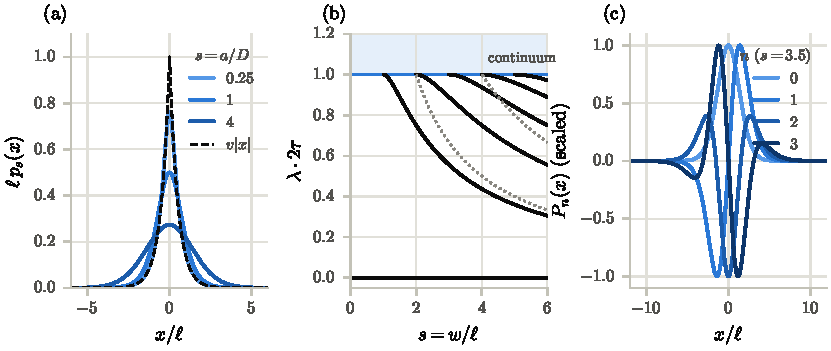
\includegraphics[width=\linewidth]{lncosh.pdf}
  \caption{The soft V, $U=a\ln\cosh(x/w)$, with lengths in $\ell=D/v$.
  (a)~Stationary densities; dashed, the sharp V ($s\to0$).
  (b)~Discrete rates in units of the continuum edge $1/2\tau$ against $s=w/\ell$. A new level leaves the edge at
  each integer $s$; dotted, the OU values $nk=2n/s$.
  (c)~The four bound states at $s=3.5$, with alternating parity.}
  \label{fig:lncosh}
\end{figure}

% ==============================================================================
\section{A well with its own walls: \texorpdfstring{$U=-a\ln\cos(x/w)$}{U = -a ln cos(x/w)}}
\label{sec:lncos}

\begin{keyresults}
$A=-(a/w)\tan(x/w)$, $B=D$ on $|x|<\pi w/2$. The potential diverges at the walls $x=\pm L/2$, $L=\pi w$. The
curvature at the bottom is $k=a/w^2$, and $s=a/D$.
\begin{align}
  p_s(x) &= \frac{\Gamma(s+1)}{\sqrt\pi\,\Gamma(s+\frac12)\,w}\cos^{2s}(x/w) \\
  Q_n &= \sqrt{\frac{n!\,(n+s)\,\Gamma(2s)}{s\,\Gamma(n+2s)}}\;C_n^{(s)}\bigl(\sin(x/w)\bigr)\quad\text{(Gegenbauer)},\qquad
  P_n=p_sQ_n \\
  \lambda_n &= \frac{D}{2w^2}\,n(n+2s)=nk+\frac{n^2\pi^2D}{2L^2}\quad\text{(exactly)} \\
  \avg{\sin(x(t)/w)} &= \sin(x_0/w)\,e^{-\lambda_1t},\qquad \lambda_1=k+\frac{\pi^2D}{2L^2}
\end{align}
For $s\ge\frac12$ the walls are never reached (they are entrance boundaries), and no wall condition is needed.
\end{keyresults}

\paragraph{Physical picture.} Two physical systems give exactly this potential.
\begin{itemize}
  \item \textbf{Rotational diffusion in three dimensions.} The polar angle $\theta$ of a unit vector diffusing on
        a sphere obeys this equation with $x=\theta-\pi/2$, $w=1$ and $s=\tfrac12$. Here
        $\mathcal U=-k_BT\ln\sin\theta$ is again entropic: the circle of latitude at $\theta$ has circumference
        $\propto\sin\theta$. The Gegenbauer polynomials become Legendre polynomials, the rates are $D_rn(n+1)$ with
        the rotational diffusion coefficient $D_r=D/2$, and $\avg{\cos\theta(t)}=\cos\theta_0\,e^{-2D_rt}$ is
        Debye's dielectric relaxation (checked by the script). On a sphere in $d$ dimensions, $s=(d-2)/2$.
  \item \textbf{Population genetics:} the Wright--Fisher allele frequency with symmetric mutation, below.
\end{itemize}

\paragraph{From Gardiner.} $p_s$ is \G{5.2.39}. Whether the walls need a condition is decided by Feller's
classification of boundaries \Gs{5.2.1e}. The spectrum and eigenfunctions are not in the book.

\subsection{Between a box and a parabola}

\begin{itemize}
  \item As $s\to0$ the potential vanishes except at the walls, and $\lambda_n\to n^2\pi^2D/2L^2$: the reflecting
        interval of length $L$ (\cref{sec:reflecting}). As $s\to\infty$ at fixed $k$ the problem becomes OU
        (\cref{sec:ou-line}). For every $s$ the exact spectrum is the sum of the two,
        $\lambda_n=nk+n^2\pi^2D/2L^2$: the confinement by the curvature and the confinement by the walls add
        (\cref{fig:lncos}b).
  \item The ladder is that of \cref{sec:solvable}, with $s\to s+1$ and $R=(D/2w^2)(2s+1)$. The slowest backward
        eigenfunction is $Q_1=\sqrt{2s+2}\,\sin(x/w)$, so $\avg{\sin(x/w)}$ relaxes as a single exponential, like
        $\avg x$ in OU. The factor in $Q_n$ is the Gegenbauer norm against the weight $(1-y^2)^{s-1/2}$, which is
        $p_s$ in $y=\sin(x/w)$. As $s\to0$ it turns $C_n^{(s)}$ into $\sqrt2\,T_n$, a Chebyshev polynomial, and
        $Q_n$ into the reflecting interval's $\sqrt2\cos(n\pi x'/L)$, $x'=x+L/2$, up to sign (\cref{sec:reflecting}).
  \item The walls are made by the potential. Near $x=L/2$ the drift is about $-sD/(L/2-x)$, the radial repulsion
        of \cref{sec:radial} with $d=2s+1$. For $s\ge\frac12$ ($d\ge2$) the particle never reaches the walls, and
        no condition is needed or possible; for $s<\frac12$ it does reach them, and the box assumes reflection. For
        $s\le-\frac12$ ($d\le0$) the potential pulls the particle into the walls, which become exits; $s=-\frac12$ is
        Wright--Fisher without mutation, in which an allele is lost or fixed for good (\cref{sec:feller}).
  \item A bound to come in \cref{sec:general}: $U''=k\sec^2(x/w)\ge k$ everywhere, so Bakry--\'Emery gives
        $\lambda_1\ge k$. That bound misses by exactly the box term.
  \item The change of variable $y=(1+\sin(x/w))/2\in(0,1)$ turns this process into the Wright--Fisher diffusion of
        population genetics with symmetric mutation: diffusion $(D/w^2)y(1-y)$ and drift $u(1-2y)$, with
        $u=(D/w^2)(2s+1)/4$ (checked by the script). Its Jacobi-polynomial spectrum (Kimura) is the $\lambda_n$
        above. Read backwards, this is the transformation of \cref{sec:general} that makes any diffusion
        coefficient constant.
\end{itemize}

\begin{figure}[tbp]
  \centering
  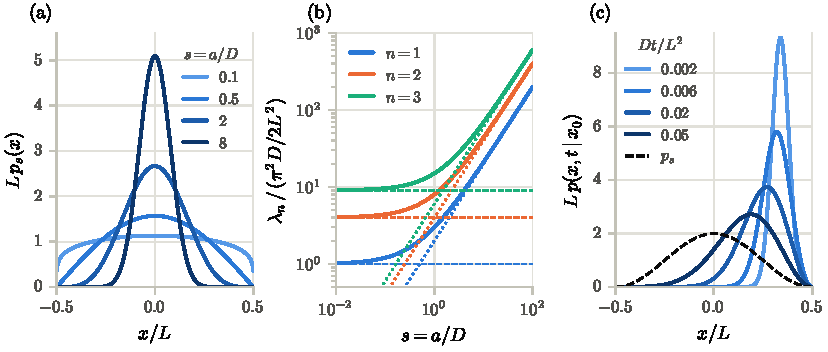
\includegraphics[width=\linewidth]{lncos.pdf}
  \caption{A well with its own walls, $U=-a\ln\cos(x/w)$, width $L=\pi w$.
  (a)~Stationary densities, from nearly uniform ($s\to0$, a reflecting box) to Gaussian.
  (b)~Rates in units of the box rate $\pi^2D/2L^2$: exactly $n^2+2sn$, the box (dashed) plus OU (dotted).
  (c)~The Gegenbauer propagator at $s=1$, from $x_0=0.35L$.}
  \label{fig:lncos}
\end{figure}

% ==============================================================================
\section{Summary of the solvable potentials}
\label{sec:solvable-summary}

\begin{itemize}
  \item Every exact spectrum in these notes comes from the factorisation $H=\mathcal A^\dagger\mathcal A$: the
        rates are those of the inverted potential, and when that is a shifted copy of the original, the spectrum
        follows by algebra.
  \item How the potential behaves at infinity decides the type of spectrum. Faster-than-linear growth (harmonic,
        harmonic plus logarithmic, walls) gives infinitely many discrete levels. Linear growth gives a continuum
        from $v^2/2D$, with finitely many levels below it (Morse, $\ln\cosh$) or infinitely many crowding up to it
        (linear plus logarithmic). No growth gives a continuum from $0$ (free motion, the logarithm alone).
  \item A logarithmic singularity of strength $c\ge D/2$ makes a boundary unreachable. The potential then
        replaces the wall condition (\cref{sec:radial,sec:lncos}). An attracting one of strength $D/2$ or more makes it
        an exit (\cref{sec:sqrt,sec:feller}).
  \item Each new potential interpolates between earlier sections: the logarithm adds dimensions to Parts~I and
        III, $\ln\cosh$ joins a V to OU, and $-\ln\cos$ joins a box to OU.
\end{itemize}

% ==============================================================================
\part{Arbitrary potentials}
\label{part:general}

\section{What holds for any potential}
\label{sec:general}

For a general $U$ (with $A=-U'$ and $B=D$), some results are exact, some are bounds, and the rest need asymptotics
or numerics. This section collects them. In applications $\mathcal U=\gamma U$ is rarely a mechanical potential.
More often it is a free energy along a reaction coordinate (a potential of mean force), for example the extension
of a molecule, a dihedral angle, or the progress of a reaction.

\paragraph{From Gardiner.} The exact results are \Gs{5.2.2}, \Gs{5.2.5} and \Gs{5.2.7}--\Gs{5.2.8} for general $A$;
the change of variables is Itô's formula \Gs{4.3.3}; the asymptotics are \Gs{5.2.7c} and Chapter~9.

\paragraph{Exact for every potential.}
\begin{itemize}
  \item The stationary state $p_s\propto e^{-2U/D}$ \G{5.2.39}, if it is normalisable \G{5.2.40}; on a circle with a
        tilt, \cref{eq:circle-ps}.
  \item Every first-passage quantity in one dimension is a quadrature (\cref{sec:fpt-toolkit}): mean exit times
        \G{5.2.158}, \G{5.2.160}, splitting probabilities (the corrected \G{5.2.190}), and conditional exit times
        \G{5.2.183}. So is the effective diffusion on a circle, \cref{eq:lifson}.
  \item The spectrum is that of $H=-\frac12D\partial_x^2+V$ with $V=U'^2/2D-U''/2$ and the wall conditions
        \cref{eq:schrodinger-walls}. It is discrete if the domain is bounded or $V\to\infty$, and otherwise has a
        continuum from the limit of $V$ at infinity (\cref{sec:operator}).
  \item Any diffusion coefficient can be made constant. In one dimension, $y=\sqrt D\int^x\dd x'/\sqrt{B(x')}$
        gives, by Itô's formula, $\dd y=\sqrt D\bigl[A/\sqrt B-B'/(4\sqrt B)\bigr]\dd t+\sqrt D\,\dd W$ (the Lamperti
        transformation). So everything here covers every one-dimensional diffusion with $B>0$;
        \cref{sec:lncos} is an example, run backwards from Wright--Fisher.
\end{itemize}

\paragraph{Bounds on the gap.}
\begin{itemize}
  \item \textbf{Upper bound.} Any trial function $f$ in the Rayleigh quotient \cref{eq:rayleigh} gives an upper bound,
        $\lambda_1\le\frac12D\int p_sf'^2\big/\int p_sf^2$. With $f=x-\avg x_s$ this is
        $\lambda_1\le D/2\operatorname{Var}_s(x)$, with equality for OU.
  \item \textbf{Lower bound.} If $U''\ge k_{\min}>0$ everywhere, then $\lambda_1\ge k_{\min}$ (Bakry--\'Emery~\cite{bakry}),
        with equality for OU. For \cref{sec:lncos} both bounds hold: $k\le\lambda_1$ and
        $\lambda_1\le D/2\operatorname{Var}_s(x)$, with $\lambda_1=k+\pi^2D/2L^2$.
  \item Neither bound helps when $U$ is not convex. In a double well $\lambda_1$ is exponentially small
        (\cref{sec:double-well}).
\end{itemize}

\paragraph{Small noise: harmonic pieces and hops.} When the barriers are large compared with the temperature
$D/2$, $V$ is close to a harmonic well near every extremum $x_*$ of $U$:
$V\approx U''(x_*)^2(x-x_*)^2/2D-U''(x_*)/2$. The low spectrum is then a union of OU ladders, one per
extremum (the semiclassical limit).
\begin{itemize}
  \item Each minimum contributes $nU''$, $n=0,1,2,\dots$
  \item Each maximum contributes $(n+1)|U''|$: the barrier-top modes of \cref{sec:cos-circle}, in which a density
        slides off the hilltop.
  \item The $n=0$ levels of the minima, one per well, split into $0$ and exponentially small hopping rates. These
        are given by Kramers' formula \G{5.2.174} for a smooth barrier top, modified for a wall
        (\cref{sec:ou-mixed}) or a cusp (\cref{sec:ou-circle}).
\end{itemize}
The cosine well on a circle and the double well of \cref{sec:double-well} both follow this pattern.

\paragraph{Numerics.} The symmetrised form turns the operator into a symmetric matrix.
\begin{itemize}
  \item Discretise with jump rates $(D/2h^2)e^{-(U_j-U_i)/D}$ between neighbouring sites $i$ and $j$. Detailed
        balance with $\pi_i\propto e^{-2U_i/D}$ then holds exactly, so the zero mode is exact and exponentially
        small rates come out with relative accuracy. The symmetrised matrix is tridiagonal, with off-diagonal
        $-D/2h^2$ and diagonal the total rate of leaving each site. The script uses this for
        \cref{sec:double-well}.
  \item With orthonormal eigenfunctions $\psi_n$ of $H$, the propagator is
        \begin{equation}
          p(x,t\given x_0,0)=\sqrt{\frac{p_s(x)}{p_s(x_0)}}\;\sum_n\psi_n(x)\,\psi_n(x_0)\,e^{-\lambda_nt},
          \label{eq:sym-prop}
        \end{equation}
        which is \G{5.2.88} with Gardiner's $P_n=\sqrt{p_s}\,\psi_n$ and $Q_n=\psi_n/\sqrt{p_s}$ \cref{eq:PQ-psi},
        and the general version of Mehler's formula (\cref{sec:ou-line}). The discrete version is exact as it
        stands: the eigenvectors of the symmetrised matrix, divided or multiplied by $\sqrt{\pi_i}$, are $Q_n$ and
        $P_n$ on the grid.
\end{itemize}

% ==============================================================================
\section{Worked example: the double well}
\label{sec:double-well}

\begin{keyresults}
$U=\Delta U\,[(x/a)^2-1]^2$, $B=D$ on the line. The minima at $\pm a$ have $U''(\pm a)=8\Delta U/a^2$; the barrier
top at $0$ has $|U''(0)|=4\Delta U/a^2$. The barrier in units of the temperature is $\beta=2\Delta U/D$.
\begin{align}
  \lambda_1 &\simeq \frac{D/2}{\frac14\int_{-a}^{a}\dd x/p_s}\quad\text{\G{9.2.18}} \\
  &\simeq 2\,\frac{\sqrt{U''(a)\,|U''(0)|}}{2\pi}\,e^{-\beta}\quad\text{(Kramers)} \\
  \lambda_2 &\to |U''(0)|\ \ \text{(barrier top)},\qquad \lambda_3\to U''(a)\ \ \text{(each well)} \\
  P_0 &= p_s,\ \ Q_0=1;\quad Q_1\simeq 2\pi_c(x)-1\ \text{(committor)},\quad P_1=p_sQ_1 \\
  T(-a\to a) &\simeq\frac2{\lambda_1} \\
  \Pr\bigl(x(t)>0\given x_0=-a\bigr) &\simeq \tfrac12\bigl(1-e^{-\lambda_1t}\bigr)
\end{align}
Here $\pi_c(x)$ is the probability of reaching the right minimum before the left one (Gardiner labels the
minima $a$ and $c$ and the barrier top $b$). The limits of $\lambda_2$ and $\lambda_3$ are for $\beta\to\infty$;
the last line holds after a short intrawell transient.
\end{keyresults}

\paragraph{Physical picture.} $\mathcal U=\Delta\mathcal U\,[(x/a)^2-1]^2$: any two-state system with a barrier.
A bead in a dual-beam optical trap hops between the two foci; Kramers' theory has been tested directly this
way~\cite{mccann}. More often $x$ is a reaction coordinate and $\mathcal U$ a free energy: an isomerisation, a
protein that folds and unfolds (Gardiner's example in \Gs{9.2.2} is the reversible denaturation of
chymotrypsinogen), or a bistable switch in a cell.

\paragraph{From Gardiner.} Chapter~9 is this problem; throughout it, Gardiner's $D$ is our $D/2$. \Gs{9.1} gives
$p_s$ \G{9.1.2}, its two-peak approximation \G{9.1.5}--\G{9.1.6}, the mean time to reach the barrier top
\G{9.1.9}, and the splitting probabilities \G{9.1.10}. Kramers' method \Gs{9.2.1} reduces the dynamics to rate
equations for the two populations \G{9.2.8}, whose relaxation rate \G{9.2.18} is $\lambda_1$ and whose two-state
form \G{9.2.16} is the last line of the box. The mean exit time is \G{5.2.160}, or \G{9.2.20}.

\subsection{Spectrum: hops, wells and the hilltop}

\begin{itemize}
  \item $\lambda_0=0$ belongs to $p_s$, $\lambda_1$ is exponentially small, and $\lambda_2,\lambda_3,\dots$ are of
        order $U''$. The ratio $\lambda_2/\lambda_1\sim e^\beta$ is the metastability: the particle equilibrates
        within a well long before it changes wells (\cref{fig:double-well}b).
  \item The small-noise rule of \cref{sec:general}: two OU ladders at the minima ($nU''(a)$, each twice) and one
        at the maximum ($(n+1)|U''(0)|$), with the two ground levels split into $0$ and $\lambda_1$. For the quartic,
        $|U''(0)|=U''(a)/2$, so the second rate is the hilltop mode, $\lambda_2\to|U''(0)|$, and the intrawell rate
        comes next, at $U''(a)$ (checked at $\beta=80$).
  \item $\lambda_1$: Kramers' formula \G{5.2.174}, with $D\to D/2$, gives the one-way hop rate
        \begin{equation*}
          r=\frac{\sqrt{U''(a)\,|U''(0)|}}{2\pi}\,e^{-\beta},
        \end{equation*}
        and the flip mode relaxes at $\lambda_1=2r$, since hops go both
        ways. Gardiner's \G{9.2.18} keeps the integral $\int\dd x/p_s$ unexpanded; it matches the exact
        $\lambda_1$ to $2\times10^{-5}$ already at $\beta=12$, while the Kramers formula has $1/\beta$ corrections
        ($2.5\,\%$ at $\beta=16$).
  \item From a minimum, the mean time to reach the other minimum is $T=2/\lambda_1$, one hop at rate $r$
        (checked by quadrature of \G{5.2.160}).
\end{itemize}

\subsection{The slow mode is the committor}

\begin{itemize}
  \item The backward eigenfunction $Q_1$ is a step: about $-1$ in the left well and $+1$ in the right, switching
        across the barrier (\cref{fig:double-well}d). It is $2\pi_c-1$, with $\pi_c$ the splitting probability
        \G{9.1.10} of the box. The reason is that $\lambda_1\approx0$ makes the eigen-equation
        $\mathcal L^\dagger Q_1=-\lambda_1Q_1$ nearly the equation $\mathcal L^\dagger\pi_c=0$ of the splitting
        probability (checked to $3\times10^{-4}$ at $\beta=8$).
  \item $2\pi_c-1$ is $\pm1$ wherever $p_s$ is not negligible, so $\int p_s(2\pi_c-1)^2\,\dd x\approx1$: the committor is
        already normalised as \G{5.2.80} asks (to $10^{-3}$ at $\beta=8$). $P_1=p_sQ_1$ is $p_s$ with the sign of the
        left peak reversed.
  \item So the slowest observable is which well the particle is committed to. Keeping $P_0Q_0$ and $P_1Q_1$ in
        \G{5.2.88},
        \begin{equation*}
          p(x,t\given x_0,0)\approx p_s(x)\bigl[1+Q_1(x)\,Q_1(x_0)\,e^{-\lambda_1t}\bigr].
        \end{equation*}
        From $x_0=-a$, $Q_1(x_0)=-1$, and the probability of being on the right is $\tfrac12(1-e^{-\lambda_1t})$ after a
        brief intrawell transient (\cref{fig:double-well}c): a two-state system, left well $\rightleftharpoons$ right well,
        with rate $r$ each way, as in \G{9.2.16}.
  \item The faster modes are local. By the small-noise rule of \cref{sec:general}, the $\psi_n$ of
        \cref{eq:PQ-psi} are harmonic-oscillator states centred on an extremum: for $\lambda_2$ on the hilltop (at
        $\beta=80$, all but $2\times10^{-5}$ of $\psi_2^2$ lies within $a/4$ of it), for $\lambda_3$ in each well. So
        $P_2=\sqrt{p_s}\,\psi_2$ is a small density bump on the barrier top, and $Q_2$ is large there.
\end{itemize}

\subsection{From this potential to any}

The structure carries over to any potential with several wells: one slow rate per extra well, with a Kramers
prefactor at each saddle; fast rates from local OU ladders at every extremum; and slow eigenfunctions that are
committors. The solvable examples of these notes fit inside this picture. OU has one well and no hops. The cosine
well on a circle has one well on a loop, so its hops change the winding instead of the well
(\cref{sec:cos-circle}). The double well has two wells, and its hops change the well.

\begin{figure}[tbp]
  \centering
  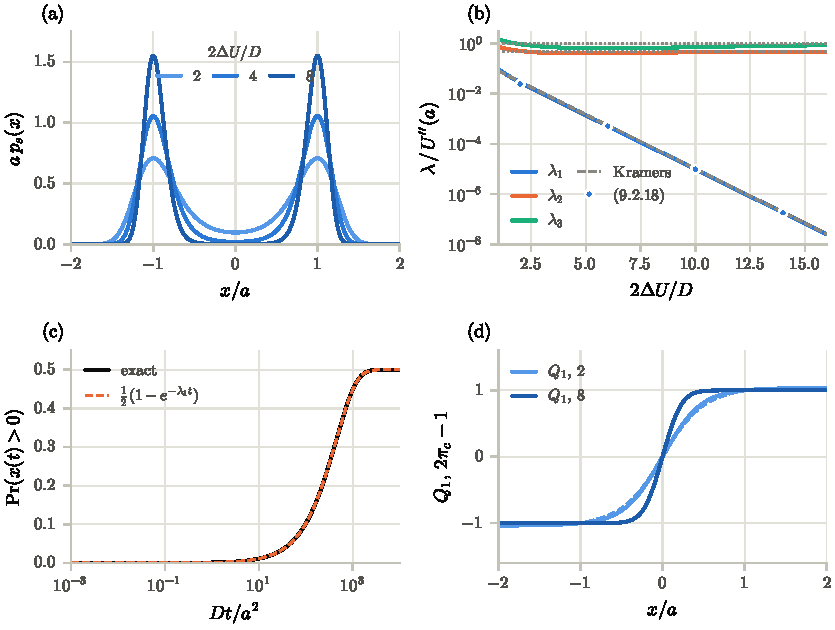
\includegraphics[width=\linewidth]{double_well.pdf}
  \caption{The quartic double well, $\beta=2\Delta U/D$.
  (a)~Stationary densities.
  (b)~The three slowest rates against the barrier, in units of $U''(a)$: $\lambda_1$ (exact; dashed, Kramers; dots,
  Gardiner's \G{9.2.18}) falls exponentially. $\lambda_2$ tends to the hilltop value $|U''(0)|/U''(a)=\frac12$,
  and $\lambda_3$ to the intrawell value $1$ (dotted lines).
  (c)~From the left minimum at $\beta=8$: probability of being on the right, exact against the two-state form.
  (d)~The slowest backward eigenfunction (solid) and $2\pi_c-1$ (dashed) at $\beta=2$ and $8$.}
  \label{fig:double-well}
\end{figure}

% ==============================================================================
\part{Interfaces and singular boundaries}
\label{part:singular}

Parts I--III use two kinds of wall, reflecting and absorbing \G{5.2.13}--\G{5.2.14}, plus the circle, which has
none. Part IV met walls that a diverging potential makes for itself (\cref{sec:radial,sec:lncos}). Gardiner's list
in \Gs{5.2.1} has three more items: conditions at a discontinuity of the coefficients \Gs{5.2.1c}; boundaries
whose type the equation itself prescribes, because $B$ vanishes there \Gs{5.2.1e}; and boundaries at infinity
\Gs{5.2.1f}, including a current that leaves at $+\infty$ and comes back at $-\infty$ \G{5.2.33}. This part works
one exactly solvable example of each (\cref{sec:interface,sec:sqrt,sec:qif}), then sorts every boundary in the notes
into Feller's four types (\cref{sec:feller}).

% ==============================================================================
\section{A step in the diffusion coefficient}
\label{sec:interface}

\begin{keyresults}
$A=0$ and $B=D_\pm$ for $\pm x>0$, on the line: free diffusion (\cref{sec:line}) on each side of an interface at
$x=0$. There the current is continuous and the density jumps by a fixed factor \Gs{5.2.1c},
\begin{equation}
  J(0^+)=J(0^-),\qquad p(0^+)=K\,p(0^-),\qquad K=\Bigl(\frac{D_-}{D_+}\Bigr)^{1-\chi},
  \label{eq:interface}
\end{equation}
with $\chi=1$ for a thermal particle (Gardiner's \G{5.2.16}), $\chi=\frac12$ for Stratonovich noise and $\chi=0$ for
It\^o noise. With $g_\pm$ the Gaussian of variance $D_\pm t$, a start at $x_0>0$, $\eta=K\sqrt{D_+/D_-}$ and
$r=(\eta-1)/(\eta+1)$:
\begin{align}
  p(x,t\given x_0,0) &= \begin{cases} g_+(x-x_0)+r\,g_+(x+x_0), & x>0\\[2pt]
  (1-r)\,g_-\bigl(x-x_0\sqrt{D_-/D_+}\bigr), & x<0\end{cases}
  \label{eq:interface-p}\\
  \text{box }(-a,a)\text{, reflecting} &:\quad p_s=\frac{1}{a(1+K)}\ \ (x<0),\qquad \frac{K}{a(1+K)}\ \ (x>0) \\
  &\phantom{:}\ Q_\lambda\propto\frac{\cos k_\pm(a-|x|)}{\cos k_\pm a}\ (\pm x>0),\ \ k_\pm=\sqrt{2\lambda/D_\pm},\ \
  P_\lambda=p_sQ_\lambda \notag\\
  \text{box }(-a,a)\text{, absorbing, from }0 &:\quad \pi_+=\frac{KD_+}{D_-+KD_+},\qquad
  T=\frac{a^2(1+K)}{D_-+KD_+}=\frac{a^2}{\avg{B}_s}
\end{align}
From the interface, $T$ is $a^2$ divided by the arithmetic (thermal), geometric (Stratonovich) or harmonic (It\^o)
mean of $D_+$ and $D_-$. A potential step $\Delta U=U(0^+)-U(0^-)$ at fixed $D$ gives $K=e^{-2\Delta U/D}$ and
$r=-\tanh(\Delta U/D)$.
\end{keyresults}

\paragraph{Physical picture.} A tracer crossing from one medium into another at the same temperature: a colloid
moving from water into a more viscous layer, a protein entering a crowded compartment, a molecule passing between a
gel and free solution. The friction, and so $D=2k_BT/\gamma$, jumps at the interface. Which density is continuous
depends on where the noise comes from (\cref{sec:interface-conventions}).
\begin{itemize}
  \item A thermal particle has Boltzmann's density at equilibrium, which does not depend on the friction, so $p$ is
        continuous ($K=1$). Colloids near a wall, where hydrodynamics lowers $D$, behave this way~\cite{volpe}.
  \item A run-and-tumble bacterium whose swimming speed $u$ varies, tumbling at a fixed rate, piles up where it is
        slow: $p_s\propto1/u$~\cite{tailleur}. Its $B$ is $\propto u^2$, so $p_s\propto1/\sqrt B$, the Stratonovich
        case.
  \item A hopper that waits at each site for a time set by that site, then jumps left or right with equal
        probability, spends its time where hopping is slow: $p_s\propto1/B$, the It\^o case.
\end{itemize}
If the two media also differ in free energy, as when a drug dissolves better in a membrane than in water, $K$ is the
equilibrium partition coefficient~\cite{crank}. A finite step in $\mathcal U$ interpolates between the walls of
\cref{fig:walls}: an infinitely high step is a hard wall, an infinitely deep one a cliff. With $K=1$ the same
equations describe heat flowing along two rods of different conductivity, joined end to end: temperature and heat
flux are continuous.

\paragraph{From Gardiner.} \G{5.2.15}--\G{5.2.16} (and \G{5.3.18} in several dimensions) ask for continuous current
and continuous density. Both are right for a jump in $A$, as at the cusp of \cref{sec:ou-circle}. For a jump in $B$
the second is an extra physical input, not a consequence of \G{5.2.6}. If $A$ is bounded, $J=Ap-\frac12\partial_x(Bp)$
stays finite only if $Bp$ is continuous, which is the It\^o case. $p$ is continuous only when $A$ contains the
noise-induced drift $\frac12B'$, which at a step is a $\delta$-function of weight $\frac12(D_+-D_-)$. That is the
drift of a thermal particle: eliminating the velocity when the friction depends on position gives
$A=-\mathcal U'/\gamma+\frac12B'$~\cite{sancho}, and with it Gardiner's conditions. The stationary density is
\G{5.2.39}. The splitting probability and the exit time are the corrected \G{5.2.190} and \G{5.2.158}, with
$\psi=Bp_s$ piecewise constant. The backward conditions at such a surface are among the ``other boundaries'' that
\Gs{5.2.4c} sets aside; they are derived below.

\subsection{A partial image}

On each side the equation is free. So try the image construction of \cref{sec:hl-reflecting,sec:hl-absorbing} with
an image of unknown weight $r$, and on the far side a transmitted Gaussian of unknown weight. Away from the interface
$J=-\frac12D_\pm\partial_xp$, so the conditions \cref{eq:interface} read $p(0^+)=Kp(0^-)$ and
$D_+\partial_xp(0^+)=D_-\partial_xp(0^-)$. A transmitted Gaussian centred at $x_0\sqrt{D_-/D_+}$ has, at the
interface, the same exponent $(x-\text{centre})^2/2D_\pm t$ as the incident one. Both conditions then hold at all
times at once, and they fix the transmitted weight at $1-r$ and $r$ at the value in the box.
\begin{itemize}
  \item $r=+1$ is a reflecting wall (\cref{sec:hl-reflecting}), $r=-1$ an absorbing one (\cref{sec:hl-absorbing}),
        and $r=0$ no interface. Every interface lies in between.
  \item For a thermal particle, a medium in which it can hardly move ($D_-\to0$) acts as a hard wall, $r\to1$, and
        one that sweeps it away ($D_-\to\infty$) acts as a cliff, $r\to-1$. In the It\^o case the signs are
        reversed: the slow side traps.
  \item In the Stratonovich case $\eta=1$, so $r=0$ for every ratio $D_-/D_+$: nothing is reflected.
  \item The slope of $p$ jumps by the factor $D_-/D_+$ (\cref{fig:interface}a). This is Gardiner's remark that ``the
        derivatives of $p$ are not necessarily continuous''.
  \item In $y=\int\dd x/\sqrt B$, which is $x/\sqrt{D_\pm}$ on each side (Lamperti, \cref{sec:general}), the noise is
        the same everywhere and the interface is a semi-permeable mirror. This is \emph{skew Brownian motion}: from
        the interface the particle goes right with probability $(1+r)/2=\eta/(1+\eta)$~\cite{lejay}.
\end{itemize}
A start at $x_0<0$ follows by exchanging the sides, $D_+\leftrightarrow D_-$ and $K\to1/K$. In the box $(-a,a)$ with
reflecting walls the modes are $\cos$ on each side (the $Q_\lambda$ of the box, \cref{sec:interface-backward}), and the
rates solve $K\sqrt{D_+}\tan\bigl(a\sqrt{2\lambda/D_+}\bigr)+\sqrt{D_-}\tan\bigl(a\sqrt{2\lambda/D_-}\bigr)=0$. Like
the root condition of \cref{sec:drift-mixed}, this is where the images stop giving a closed form.

\subsection{Which density is continuous}
\label{sec:interface-conventions}

Smooth the step over a width $\varepsilon$. Then $B$ is smooth, every reading of the noise gives an ordinary
equation, and the readings differ only by a drift $\chi B'/2$:
\begin{itemize}
  \item It\^o, $\dd x=\sqrt B\,\dd W$ ($\chi=0$): $x$ is a martingale, and $p_s\propto1/B$;
  \item Stratonovich, $\dd x=\sqrt B\circ\dd W$ ($\chi=\frac12$): $p_s\propto1/\sqrt B$;
  \item thermal, also called H\"anggi--Klimontovich or isothermal ($\chi=1$): $p_s$ is uniform.
\end{itemize}
In each case \G{5.2.39} gives $\psi=B^\chi$ and $p_s=\psi/B\propto B^{\chi-1}$ (\cref{fig:interface}b). As
$\varepsilon\to0$ the extra drift becomes a $\delta$-function of weight $\chi(D_+-D_-)/2$. It is too thin to change
the motion on either side, but strong enough to set the jump of $p$, to $K=(D_-/D_+)^{1-\chi}$. So a sharp
interface remembers how the step was smoothed. The script solves the smoothed equation by finite differences and
recovers the closed form \cref{eq:interface-p}, with an error proportional to $\varepsilon$; simulations of the
smoothed SDE give the exit probabilities (\cref{fig:interface}c).

\subsection{Backward conditions and exit from a box}
\label{sec:interface-backward}

Pair the forward and backward equations as in \cref{eq:green}, treating the interface as two walls. What is left at
$x=0$ is $J\,[f]_{0^-}^{0^+}+\frac12p(0^-)\bigl[KD_+f'(0^+)-D_-f'(0^-)\bigr]$. So a backward function is continuous
at the interface, with $KD_+f'(0^+)=D_-f'(0^-)$.

These are the conditions on Gardiner's $Q_\lambda$. In the reflecting box, $Q_\lambda=\cos k_\pm(a-|x|)/\cos k_\pm a$
on each side has $Q'=0$ at the walls and $Q(0^\pm)=1$, so it is continuous; the derivative condition is the root
condition above. $P_\lambda=p_sQ_\lambda$ then jumps by $K$, like $p_s$, and carries a continuous current: it meets
the forward conditions \cref{eq:interface}, which pair with the backward ones as the wall conditions do. The script
checks that these $P_\lambda$, $Q_\lambda$ are biorthonormal for $\chi=1$ and $0$.

With absorbing walls at $\pm a$:
\begin{itemize}
  \item $\pi_+$ is piecewise linear, with slopes in the ratio $D_-:KD_+$ (\cref{fig:interface}c). In the It\^o case
        $x$ is a martingale, so $\pi_+(x_0)=(x_0+a)/2a$ whatever $B$ does.
  \item $T$ is piecewise quadratic. From the interface it is $a^2/\avg B_s$, where
        $\avg B_s=(D_-+KD_+)/(1+K)$ is the average of $B$ over the stationary density of the reflecting box. The
        reason: in all three readings $x^2-\int_0^tB\,\dd t'$ is a martingale (the extra drift acts only where
        $x=0$), so $a^2=\avg{\int_0^TB\,\dd t}$, and from $x_0=0$ the times spent on the two sides before exit are in
        the ratio $K:1$.
  \item A thermal particle released at the interface leaves through the fast side with probability
        $D_+/(D_++D_-)$, after a mean time $2a^2/(D_++D_-)$.
\end{itemize}

\begin{figure}[tbp]
  \centering
  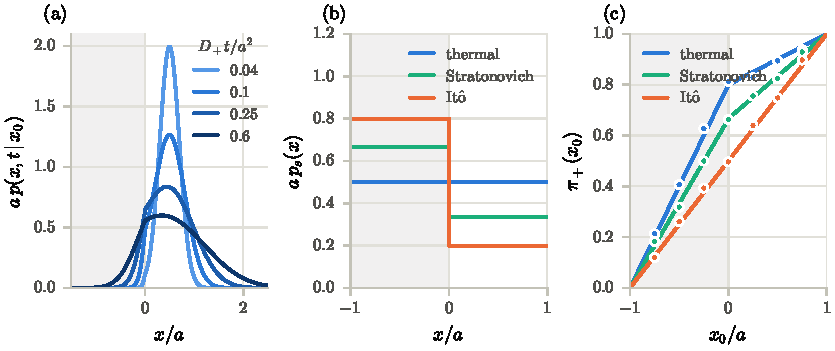
\includegraphics[width=\linewidth]{interface.pdf}
  \caption{A step in the diffusion coefficient, $D_-=D_+/4$; the slow side is shaded.
  (a)~A thermal particle from $x_0=a/2$. $p$ is continuous at the interface, and its slope jumps by the factor $4$.
  (b)~Stationary densities in the box $(-a,a)$ with reflecting walls, for the three readings of the noise.
  (c)~Probability of leaving the box through $+a$. Lines are the closed forms; dots are simulations of the smoothed
  equation ($\varepsilon=0.03a$, 1000 paths per point).}
  \label{fig:interface}
\end{figure}

% ==============================================================================
\section{Where \texorpdfstring{$B$}{B} vanishes: the square-root process}
\label{sec:sqrt}

\begin{keyresults}
$A=dD-2ky$, $B=4Dy$ on $y>0$, for any real $d$: the squared radius $y=r^2$ of \cref{sec:radial}, and the equation
Feller studied in 1951~\cite{feller51}. Lengths in $\ell^2=D/k$, times in $1/k$. With $\mu=d/2-1$,
$\bar y_t=y_0e^{-2kt}$, $\sigma_t^2=\frac12\ell^2(1-e^{-2kt})$ and $z_t=\bar y_t/2\sigma_t^2=(y_0/\ell^2)/(e^{2kt}-1)$.
The origin is an exit for $d\le0$, regular for $0<d<2$ and an entrance for $d\ge2$; infinity is natural. The
propagator is $p_+$ when the process is reflected ($d>0$) and $p_-$ when it is absorbed ($d<2$):
\begin{align}
  p_\pm(y,t\given y_0,0) &= \frac{1}{2\sigma_t^2}\Bigl(\frac{y}{\bar y_t}\Bigr)^{\mu/2}
  e^{-(y+\bar y_t)/2\sigma_t^2}\,I_{\pm\mu}\Bigl(\frac{\sqrt{y\bar y_t}}{\sigma_t^2}\Bigr) \label{eq:sqrt-p}\\
  \text{reflected} &:\quad p_s=\frac{y^{d/2-1}e^{-y/\ell^2}}{\Gamma(d/2)\,\ell^{d}},\quad \lambda_n=2nk,\quad
  Q_n\propto L_n^{(\mu)}(y/\ell^2),\quad P_n=p_sQ_n \\
  \text{absorbed} &:\quad S=P\bigl(1-\tfrac d2,z_t\bigr),\quad \lambda_n=(2n+2-d)k \\
  &\phantom{:}\quad Q_n\propto y^{1-d/2}L_n^{(1-d/2)}(y/\ell^2),\quad P_n\propto e^{-y/\ell^2}L_n^{(1-d/2)}(y/\ell^2) \\
  \text{QSDs} &:\quad q_\lambda\propto M\bigl(1+\tfrac{\lambda}{2k},2-\tfrac d2,-y/\ell^2\bigr),\quad
  0<\lambda\le(2-d)k
\end{align}
$P(a,z)=\gamma(a,z)/\Gamma(a)$ is the regularised incomplete gamma function and $M$ is Kummer's function. Point starts
reach the QSD $e^{-y/\ell^2}/\ell^2$. For $d=0$, $\Pr(y_t=0)=e^{-z_t}$: the extinction probability of Feller's
branching diffusion.
\end{keyresults}

\paragraph{Physical picture.} Four systems lead to this equation.
\begin{itemize}
  \item The squared distance from the centre of an overdamped particle in an isotropic harmonic trap in $d$
        dimensions (\cref{sec:radial}), or its potential energy $E=\frac12\mathcal Kr^2$. $E/k_BT$ is gamma
        distributed with mean $d/2$, which is equipartition. For $d=2$, $y$ is the intensity of a noisy optical field,
        exponentially distributed.
  \item A population with demographic noise. Births and deaths at nearly equal per-capita rates make the variance of
        the change proportional to the size, $B\propto y$; $2k$ is the net death rate and $dD$ a rate of immigration.
        With no immigration ($d=0$) this is Feller's branching diffusion, which dies out for sure. Gardiner's reaction
        $X+A\rightleftharpoons2X$ \G{5.2.57} behaves the same way near $x=0$: with no $X$ there is no reaction.
  \item The interest rate of Cox, Ingersoll and Ross~\cite{cir}, $\dd y=(a-by)\,\dd t+\sigma\sqrt y\,\dd W$, which is
        this equation with $d=4a/\sigma^2$. Their condition $2a\ge\sigma^2$, that the rate never reaches zero, is
        $d\ge2$.
  \item In the radius $r=\sqrt y$, the logarithmic potential $-(d-1)k_BT\ln r$ of \cref{sec:radial} attracts when
        $d<1$. A counterion near a thin charged rod, moving in the plane perpendicular to it, feels
        $\mathcal U=2\xi_{\rm M}k_BT\ln r$, where $\xi_{\rm M}$ is the Manning parameter. With the entropic term of the
        plane, this is $d=2-2\xi_{\rm M}$. For $\xi_{\rm M}\ge1$ the rod is an exit boundary and the counterions
        collapse onto it: Manning condensation~\cite{manning}, for a rod of zero radius.
\end{itemize}

\paragraph{From Gardiner.} This is a prescribed boundary \Gs{5.2.1e}: $B(0)=0$, and the equation decides whether a
condition may be imposed there. Gardiner's quick rule \G{5.2.22}--\G{5.2.24}, by the sign of $A(0)$, assumes that
$\sqrt B$ is Lipschitz, which forces $\partial_yB(0)=0$ \G{5.2.20}. Here $\partial_yB(0)=4D$, and the rule fails:
$A(0)=dD>0$ for every $d>0$, but only $d\ge2$ is an entrance. Feller's criteria \G{5.2.25}--\G{5.2.29} decide the
type (below). The paragraph after them has a misprint: its second ``exit'' should read ``entrance''.
\begin{itemize}
  \item For $d=2$ this is the square of the Rayleigh process of \Gs{5.2.6d}, with the same Laguerre spectrum
        \G{5.2.133}.
  \item Gardiner's reaction model \G{5.2.57}--\G{5.2.60} has $A(0)=0$ and $\partial_xB(0)>0$, which is the $d=0$ case:
        an exit. Its stationary solution \G{5.2.59} behaves like $1/x$ at $x=0$ and is not normalisable, like
        $y^{d/2-1}$ here.
  \item The mean time to reach $0$ is \G{5.2.161}, with the reflecting wall at infinity.
  \item Gardiner's backward reflecting condition \G{5.2.69} carries the proviso ``unless $B$ vanishes''. Here it
        becomes $\psi\,\partial_yf\to0$: a zero derivative with respect to the scale $\int\dd y/\psi$.
\end{itemize}

\subsection{Feller's test}
\label{sec:feller-test}

Gardiner's functions \G{5.2.25}--\G{5.2.28} are, up to constant factors,
\begin{equation}
  f=y^{-d/2}e^{y/\ell^2},\qquad g=\frac{2}{Bf}=\frac{y^{d/2-1}e^{-y/\ell^2}}{2D}.
\end{equation}
Here $f=1/\psi$ is the density of the scale $\int\dd y/\psi$, and $g=2\psi/B$ is twice the zero-current solution
\cref{eq:ps}; Feller calls them the scale and speed densities. Near $y=0$:
\begin{itemize}
  \item $f$ is integrable iff $d<2$, and $g$ iff $d>0$;
  \item $h_1=f\int_{y_0}^yg$ is integrable iff $d<2$. This is the condition for the boundary to be reachable from
        inside;
  \item $h_2=g\int_{y_0}^yf$ is integrable iff $d>0$. This is the condition for a process started at the boundary to
        leave it.
\end{itemize}
Gardiner's table then gives exit for $d\le0$, regular for $0<d<2$, and entrance for $d\ge2$. At $y\to\infty$, $f$
grows and $g$ decays like $e^{\pm y/\ell^2}$, and neither $h_1$ nor $h_2$ is integrable: a natural boundary. The
script evaluates the four integrals with shrinking cutoffs and finds the same types, in $y$ and in $r$.

\subsection{From the radius: two solutions}

The density of $y=r^2$ is $p_r(\sqrt y)/2\sqrt y$, and this turns the radial propagator of \cref{sec:radial} into
$p_+$. In $r$ the noise is constant and the drift $(d-1)D/2r-kr$ is singular. In $y$ the drift is smooth and the
noise vanishes. The boundary has the same type in both, because Feller's integrals do not change under a change of
variable: the type belongs to the process, not to the coordinate.

The second solution, $p_-$, has $I_{-\mu}$ in place of $I_\mu$. It is the Doob transform (\cref{sec:hl-absorbing}) of
the process in dimension $4-d$,
\begin{equation}
  p_-^{(d)}(y,t\given y_0)=e^{-(2-d)kt}\Bigl(\frac{y_0}{y}\Bigr)^{1-d/2}p_+^{(4-d)}(y,t\given y_0),
\end{equation}
which for $d=1$ is the relation found in \cref{sec:radial} between OU absorbed at its bottom and the radius in three
dimensions. Both functions solve the equation for every $d$; the type of boundary decides which one is the answer
(\cref{fig:sqrt}).
\begin{itemize}
  \item \textbf{Entrance, $d\ge2$.} From $y_0>0$ the origin is never reached. Started at $y_0=0$, the process enters
        at once: $p_+$ tends to a gamma density of scale $2\sigma_t^2$. Only $p_+$ is a probability density, so there is
        nothing to choose, and no condition can be imposed.
  \item \textbf{Regular, $0<d<2$.} The origin is reached in finite time and can be left, and both solutions are
        legitimate, so a condition must be chosen. Reflection, $J(0)=0$, gives $p_+$, which diverges at the origin
        like $y^{d/2-1}$. Absorption gives $p_-$, which tends to a nonzero constant there (\cref{fig:sqrt}c). So where
        $B$ vanishes an absorbing boundary does not have $p=0$ \G{5.2.14}. What vanishes is $p/p_s$, the backward
        function, as the operator picture of \cref{sec:operator} suggests. Partly absorbing and sticky conditions are
        also possible at a regular boundary; they are not needed here.
  \item \textbf{Exit, $d\le0$.} The origin is reached in finite time and never left, and $p_-$ is the only
        solution. The zero-current solution $y^{d/2-1}e^{-y/\ell^2}$ is not normalisable, so nothing can be
        reflected, and probability collects at $y=0$ as an atom of mass $1-S$.
\end{itemize}
For $d=1$ the regular case and its two choices are \cref{sec:ou-hl-reflecting,sec:ou-hl-absorbing}, squared.

\subsection{Spectrum, survival and QSDs}

\begin{itemize}
  \item The reflected process has the Laguerre ladder $2nk$ of \cref{sec:radial} and the gamma stationary density.
        The absorbed one has the ladder of dimension $4-d$, shifted up by $(2-d)k$ through the factor $e^{-(2-d)kt}$.
        In the regular window both ladders exist. At an exit only the absorbed one does, at an entrance only the
        reflected one (\cref{fig:sqrt}b). They meet at $d=2$, where the origin stops being reachable.
  \item \textbf{Gardiner's $P_n$ and $Q_n$.} With $z=y/\ell^2$:
        \begin{itemize}
          \item reflected: $Q_n=\sqrt{n!\,\Gamma(d/2)/\Gamma(n+d/2)}\,L_n^{(\mu)}(z)$ and $P_n=p_sQ_n$, the $Q_n$ of
                \cref{sec:radial} in the variable $r^2$;
          \item absorbed: $P_n=w\,Q_n$ with the zero-current solution $w=z^{d/2-1}e^{-z}/\ell^2$, which gives
                $Q_n=c_nz^{1-d/2}L_n^{(1-d/2)}(z)$, $P_n=c_ne^{-z}L_n^{(1-d/2)}(z)/\ell^2$ and $c_n=\sqrt{n!/\Gamma(n+2-d/2)}$.
                In the regular window $w=\Gamma(d/2)\,p_s$ is the reflected $p_s$ of \G{5.2.91}, up to a constant. At an
                exit there is no reflected problem to borrow it from, but $w$ still works as the weight, although
                it cannot be normalised.
        \end{itemize}
        At the origin the absorbed $Q_n\to0$ while $P_n$ tends to a constant: absorption where $B$ vanishes sets
        $Q=0$, not $P=0$, as found for $p_-$ above. The QSDs $q_\lambda$ with $\lambda<(2-d)k$ are forward
        eigenfunctions off the ladder; $q_\lambda/w$ grows like $e^{z}$, so they do not enter \G{5.2.88}. At
        $\lambda=(2-d)k$ the Kummer function is $e^{-z}$ and $q_\lambda\propto P_0$.
  \item Survival decays at $\lambda_0=(2-d)k$: that is $k$ for OU absorbed at its bottom ($d=1$,
        \cref{sec:ou-hl-absorbing}) and $2k$ for the branching diffusion. Integrating $p_-$ term by term in the series of
        $I_{-\mu}$ gives the incomplete gamma function of the box. With no trap ($k=0$), $z_t=y_0/2Dt$ and
        $S\simeq(y_0/2Dt)^{1-d/2}/\Gamma(2-d/2)$. This generalises the $t^{-1/2}$ of \cref{sec:hl-absorbing}, and the
        mean time to reach the origin is finite only for $d<0$.
  \item With the trap, the mean time $T(y_0)=\int_0^\infty S\,\dd t$ is finite for every $d<2$ and diverges as
        $d\to2^-$. It passes smoothly through $d=0$: seen from inside, an exit and a regular boundary look alike. They
        differ in what can happen after arrival.
  \item $y=\infty$ is natural, so the criterion of \cref{sec:spectrum-states} predicts a continuum of QSDs, as for OU
        absorbed at its bottom. The Kummer functions in the box are that continuum: each is positive, with a tail
        $y^{-1-\lambda/2k}$. A point start reaches the minimal one, at $\lambda=(2-d)k$, where $M$ reduces to
        $e^{-y/\ell^2}$: the Yaglom limit is exponential in every dimension. For $d=1$, in $x=\sqrt y$, it is the
        Rayleigh QSD. A logistic term, $A\to A-cy^2$, makes infinity an entrance, and the QSD becomes
        unique~\cite{cattiaux}.
\end{itemize}

\begin{figure}[tbp]
  \centering
  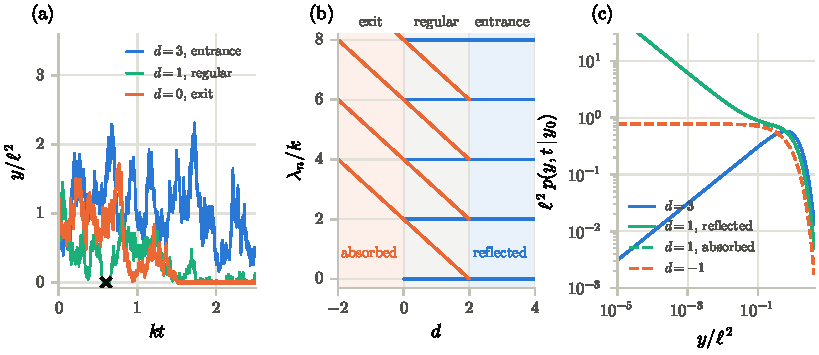
\includegraphics[width=\linewidth]{sqrt.pdf}
  \caption{The square-root process; $y$ is in units of $\ell^2=D/k$.
  (a)~Paths from $y_0=\ell^2$. $d=3$: an entrance, never reached. $d=1$: regular, reflected each time it arrives;
  absorption would stop it at the cross. $d=0$: an exit, absorbed for good. The $d=3$ and $d=1$ paths are squared radii
  of OU motions; the $d=0$ path is sampled exactly.
  (b)~Rates against $d$. The reflected ladder $2nk$ exists for $d>0$, the absorbed one $(2n+2-d)k$ for $d<2$. Only in
  the regular window do both exist, and there a condition must be chosen.
  (c)~Densities near the origin at $kt=0.25$ from $y_0=\ell^2$. The entrance density vanishes, the reflected one
  diverges like $y^{-1/2}$, and the absorbed ones tend to constants.}
  \label{fig:sqrt}
\end{figure}

% ==============================================================================
\section{A current through infinity}
\label{sec:qif}

\begin{keyresults}
$A=x^2+I$, $B=D$ on the line, in the units of the neuron model below ($x$ and $I$ dimensionless, $D$ a rate). The noise
sets the scales $D^{1/3}$ for $x$, $D^{-1/3}$ for $t$ and $D^{2/3}$ for $I$. $+\infty$ is an exit and $-\infty$ an
entrance; what leaves at $+\infty$ is reinjected at $-\infty$, $J(+\infty)=J(-\infty)=J_s$ \G{5.2.33}.
\begin{align}
  p_s(x) &= \frac{2J_s}{D}\int_x^\infty e^{\varphi(x)-\varphi(y)}\,\dd y\;\simeq\;\frac{J_s}{x^2}\ \ (x\to\pm\infty),
  \qquad \varphi=\frac2D\Bigl(\frac{x^3}3+Ix\Bigr) \\
  \frac1{J_s} &= \sqrt{\frac{2\pi}{D}}\int_0^\infty\frac{\dd u}{\sqrt u}\,
  \exp\Bigl[-\frac2D\Bigl(\frac{u^3}{12}+Iu\Bigr)\Bigr] \\
  &\to\ \frac{\pi}{\sqrt I}\ \ (D\to0,\ I>0),\qquad 6.27\,D^{-1/3}\ \ (I=0),\qquad
  \frac\pi c\,e^{8c^3/3D}\ \ (D\to0,\ I=-c^2) \notag\\
  P_0 &= p_s,\quad Q_0=1;\qquad Q_\lambda(+\infty)=Q_\lambda(-\infty);\qquad P_\lambda\neq p_sQ_\lambda\ \ (\lambda\neq0)
\end{align}
The constant is $6.27=\frac{\sqrt{2\pi}}3\,6^{1/6}\,\Gamma(\frac16)$. In $\theta=2\arctan x$ the line closes into a
circle,
\begin{equation}
  \dd\theta=\bigl[1-\cos\theta+I(1+\cos\theta)-\tfrac D2\sin\theta\,(1+\cos\theta)\bigr]\dd t+\sqrt D\,(1+\cos\theta)\,\dd W,
\end{equation}
and both infinities are the point $\theta=\pi$, where the noise vanishes and the drift is $2$.
\end{keyresults}

\paragraph{Physical picture.} The quadratic integrate-and-fire (QIF) neuron. $x$ is the membrane potential, rescaled.
It runs off to $+\infty$ in finite time, which is a spike, and is reset to $-\infty$; $J_s$ is the firing rate. The
model is the normal form of a neuron that starts firing through a saddle-node bifurcation on its limit cycle, and in
$\theta$ it is the theta neuron of Ermentrout and Kopell~\cite{ermentrout}. Mechanically, it is an overdamped
particle sliding off the cubic potential $\mathcal U=-\gamma(x^3/3+Ix)$. This is what the tilted washboard of
\cref{sec:cos-circle} looks like near its critical tilt, around the point where the minimum and the maximum merge,
seen through a coordinate that sends the rest of the circle to infinity. Each passage through infinity is one
winding: a phase slip of the overdamped pendulum or of the Josephson junction. For $I<0$ the particle sits in a well
and escapes over a barrier, as below depinning in \cref{sec:cos-circle}.

\paragraph{From Gardiner.} \Gs{5.2.1f} allows every kind of boundary of \Gs{5.2.1} at infinity, and notes that a
nonzero current there needs $A$ or $B$ to be infinite; here $A\sim x^2$. Of his two conditions, $J(\pm\infty)=0$
\G{5.2.32} and $J(+\infty)=J(-\infty)$ \G{5.2.33}, this is the second, ``the limit of periodic''.
\begin{itemize}
  \item With constant $J$ the stationary solution is \G{5.2.45}, with the seam at infinity.
  \item The mean time from $-\infty$ to $+\infty$ is \G{5.2.160}, with $a=-\infty$ reflecting, $b=+\infty$ absorbing
        and $\psi=e^\varphi$. Its inverse is $J_s$.
  \item The types of $\pm\infty$ follow from \G{5.2.25}--\G{5.2.29}. In $\theta$ they are Gardiner's sign rule
        \G{5.2.22}--\G{5.2.23}.
\end{itemize}

\subsection{An exit at \texorpdfstring{$+\infty$}{+infinity}, an entrance at \texorpdfstring{$-\infty$}{-infinity}}

With $\psi=e^\varphi$, Gardiner's functions are $f=e^{-\varphi}$ and $g=(2/D)e^{\varphi}$.
\begin{itemize}
  \item At $+\infty$, $f$ is integrable and $g$ is not, while $h_1=f\int g\simeq1/x^2$ is integrable: an exit. The
        drift $x^2$ carries the particle to infinity in the finite time $\int^\infty\dd x/x^2$, faster than the noise
        can bring it back. The process explodes.
  \item At $-\infty$ the roles swap: $g$ is integrable, and so is $h_2\simeq1/x^2$: an entrance. The particle comes
        down from $-\infty$ in finite time, as a particle in $A=-kx^3$ comes down from $+\infty$
        (\cref{sec:spectrum-states}).
  \item The mirror image $x\to-x$ turns $A$ into $-A$, that is $U$ into $-U$: the partner of \cref{sec:solvable}.
        It exchanges the two ends, and with them exit and entrance. That is true of the partner in general
        (\cref{sec:feller}).
\end{itemize}
Without reinjection the process is absorbed at $+\infty$, and $1/J_s$ is the mean time to get there from $-\infty$. It
is finite, because both ends are crossed in finite time.

\subsection{Through infinity: the circle again}

Reinjecting at $-\infty$ whatever leaves at $+\infty$ is the condition \G{5.2.33}. The stationary equation
$J=J_s$ integrates as in \G{5.2.45} to the box, and normalisation fixes $J_s$. Writing $y=s+u/2$ and $x=s-u/2$ turns
$\varphi(y)-\varphi(x)$ into $\frac2D(us^2+u^3/12+Iu)$, and the Gaussian integral over $s$ leaves the single integral
of the box~\cite{lindner}.
\begin{itemize}
  \item Without noise ($D\to0$, $I>0$) the period is $\int\dd x/(x^2+I)=\pi/\sqrt I$: the firing rate rises as
        $\sqrt I$ from the bifurcation.
  \item At the bifurcation ($I=0$) the noise alone sets the rate, $J_s\propto D^{1/3}$.
  \item Below it ($I=-c^2$) the particle sits in the well at $x=-c$ and must cross the barrier at $+c$, of height
        $\Delta U=\frac43c^3$. Kramers' formula \G{5.2.174}, with $U''=\pm2c$, gives $J_s\simeq(c/\pi)e^{-2\Delta U/D}$.
        Once over the top, the particle falls to infinity.
  \item $p_s\simeq J_s/x^2$ at both ends: the density of a particle moving at speed $x^2$ and carrying the current
        $J_s$.
  \item Gardiner's eigenfunctions. Pairing as in \cref{eq:green} leaves $-J_s\bigl[f(+\infty)-f(-\infty)\bigr]$ at the
        two ends, so the backward condition that goes with \G{5.2.33} is $Q_\lambda(+\infty)=Q_\lambda(-\infty)$:
        a function of the start must not notice the reinjection. $Q_0=1$ satisfies it, and $P_0=p_s$. Because
        $J_s\neq0$ the other $P_\lambda$ are not $p_sQ_\lambda$, as on the tilted circle of \cref{sec:cos-circle};
        both have to be found separately, and the notes do not compute them.
\end{itemize}

The angle $\theta=2\arctan x$ shows this as the circle it is. Itô's formula gives the box, with bounded
coefficients. At $\theta=\pi$, the image of both infinities, the noise vanishes like $(\theta-\pi)^4$ while the drift
is $2$. $\sqrt B$ is Lipschitz there, so \G{5.2.20} holds, and Gardiner's sign rule makes $\theta=\pi$ an exit for the
arc below it \G{5.2.22} and an entrance for the arc above \G{5.2.23}. On the circle the two are one point, which the
particle crosses without stopping, and the density there is finite, $J_s/2$ (\cref{fig:qif}c). The point is special
because $B$ vanishes there, a property of the coefficients and not of the topology (\cref{sec:circle-toolkit}). The
cut-invariant formula \cref{eq:circle-ps} assumes $B>0$ and does not apply. No probability diffuses back through
$\theta=\pi$, so the integral stops there, as in the box.

\subsection{Regular at infinity: a choice}

Infinity can also be regular. Take the free circle, or constant drift on it (\cref{sec:circle,sec:drift-circle}), with
circumference $2\pi$, and look at it through the same coordinate, $x=\tan(\theta/2)$. Then $B=\frac14D(1+x^2)^2$ and
$A=\frac12v(1+x^2)+\frac14Dx(1+x^2)$, both infinite at $\pm\infty$. Gardiner's $f\propto e^{-(4v/D)\arctan x}/(1+x^2)$
and $g\propto e^{(4v/D)\arctan x}/(1+x^2)$ are both integrable, so $\pm\infty$ are regular: reached in finite time,
and left again. A condition must be chosen, and Gardiner's two are the natural ones. \G{5.2.32}, $J(\pm\infty)=0$, is
the interval $(-\pi,\pi)$ with reflecting walls (\cref{sec:reflecting,sec:drift-reflecting}). \G{5.2.33} is the circle,
on which $p_s$ is the Cauchy density $1/\pi(1+x^2)$, carrying the current $J_s=v/2\pi$. Gardiner's description of
the two as ``the limits of reflecting and periodic boundary conditions'' is exact.

\begin{figure}[tbp]
  \centering
  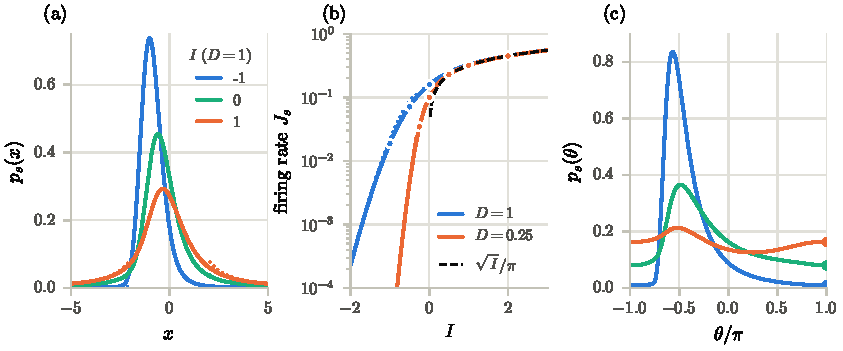
\includegraphics[width=\linewidth]{qif.pdf}
  \caption{A current through infinity: the QIF neuron.
  (a)~Stationary densities for $D=1$; dotted, the tails $J_s/x^2$.
  (b)~Firing rate against $I$: exact (solid), the noiseless $\sqrt I/\pi$ (dashed), and Kramers' formula for $I<0$
  (dotted). Dots are simulations of the $\theta$ equation.
  (c)~The densities of (a) in the angle $\theta=2\arctan x$. Both infinities are the point $\theta=\pi$, where the
  density is $J_s/2$ (dots).}
  \label{fig:qif}
\end{figure}

% ==============================================================================
\section{Feller's classification across the notes}
\label{sec:feller}

Every boundary of a one-dimensional diffusion, at a finite point or at infinity, is of one of four types. Two
questions decide the type: can the process reach the boundary from inside, and can it start there and leave? In
Gardiner's notation \G{5.2.25}--\G{5.2.29} the first holds when $h_1=f\int g$ is integrable near the boundary, the
second when $h_2=g\int f$ is, with $f=1/\psi$ and $g=2\psi/B$ (\cref{sec:feller-test}). \Cref{tab:feller} lists what
each type means and where it appears in these notes.

\begin{table}[h]
\centering
\footnotesize
\renewcommand{\arraystretch}{1.3}
\setlength{\tabcolsep}{3pt}
\begin{tabular}{@{}>{\raggedright}p{0.1\linewidth} >{\raggedright}p{0.11\linewidth} >{\raggedright}p{0.2\linewidth} >{\raggedright\arraybackslash}p{0.55\linewidth}@{}}
\toprule
Type & Reached? Left? & Condition & Examples in these notes \\
\midrule
regular & yes, yes & must be chosen: reflecting, absorbing, or gluing to another boundary \G{5.2.33} & every wall of
Parts I--III; the origin in \S\ref{sec:radial} and \S\ref{sec:sqrt} for $0<d<2$ (for $d=1$, \S\ref{sec:ou-hl-reflecting}
and \S\ref{sec:ou-hl-absorbing}); the walls of \S\ref{sec:lncos} for $|s|<\frac12$; $\pm\infty$ for a circle in the
coordinate $\tan(\theta/2)$ (\S\ref{sec:qif}) \\
exit & yes, no & none possible: absorbing & the origin in \S\ref{sec:sqrt} for $d\le0$ (branching diffusion, Gardiner's
$X+A\rightleftharpoons2X$, Manning condensation); the walls of \S\ref{sec:lncos} for $s\le-\frac12$ (neutral
Wright--Fisher); $+\infty$ for the QIF neuron \\
entrance & no, yes & none possible & the origin in \S\ref{sec:radial} and \S\ref{sec:sqrt} for $d\ge2$; the walls of
\S\ref{sec:lncos} for $s\ge\frac12$; $-\infty$ for the QIF neuron; $+\infty$ for $A=-kx^3$ \\
natural & no, no & none possible & $\pm\infty$ for free motion, constant drift, OU, $\ln\cosh$ and the double well;
$\infty$ in \S\ref{sec:radial} and \S\ref{sec:sqrt}; $0$ and $\infty$ for geometric Brownian motion \\
\bottomrule
\end{tabular}
\caption{Feller's four types of boundary, with the examples in these notes.}
\label{tab:feller}
\end{table}

\paragraph{What the table says.}
\begin{itemize}
  \item \textbf{A wall condition is a choice only at a regular boundary.} Every wall of Parts I--III is a finite point
        where $B>0$ and $A$ is bounded, so it is regular, and the notes chose reflection or absorption there. At the
        other three types the equation decides by itself, and imposing a condition is either redundant or impossible.
  \item \textbf{Stationary states and arrival times.} Near an exit the zero-current solution is not normalisable, and
        the mean time to arrive is finite. Near an entrance it can be normalised, and the mean time to arrive is
        infinite. A regular boundary allows both. This is Gardiner's remark after \G{5.2.29}, with its misprint
        corrected.
  \item \textbf{QSDs.} A unique QSD that attracts every start needs the far end to be an entrance
        (\cref{sec:spectrum-states}). OU and the square-root process have natural boundaries at infinity, hence their
        continua of QSDs.
  \item \textbf{A change of variable does not change the type.} $y=r^2$ (\cref{sec:sqrt}), Lamperti's transformation
        and $x=\tan(\theta/2)$ (\cref{sec:qif}) move a singularity from the drift to the noise, or out to infinity, but
        the integrals of \G{5.2.25}--\G{5.2.28} do not change. A boundary can look ordinary in one coordinate ($\theta=\pi$
        on a circle) and singular in another ($x=\pm\infty$).
  \item \textbf{The partner swaps exit and entrance.} With $B=D$, $U\to-U$ turns $f$ into $\frac D2g$ and $g$ into
        $\frac2Df$, so $h_1$ and $h_2$ trade places; regular and natural boundaries keep their type. Examples: the
        logarithm in dimension $d$ and in dimension $2-d$; the walls of $-a\ln\cos$ with $s$ and $-s$; the two ends of
        the QIF neuron. The partner also shares every nonzero rate (\cref{sec:solvable}). So neutral Wright--Fisher
        ($s=-\frac12$, absorbed at both ends) relaxes at exactly the rates of rotational diffusion on the sphere
        ($s=\frac12$), $\frac{D}{2w^2}n(n+1)$ with $n\ge1$, but has no zero mode: this is Kimura's spectrum.
\end{itemize}

\paragraph{Gardiner's sign rule.} Where $B$ vanishes at $a$ but $\sqrt B$ stays Lipschitz, so that
$B\simeq c\,(x-a)^2$, the sign of $A(a)$ decides the type \G{5.2.22}--\G{5.2.24}. The standard example is
$\dd x=(a_0-bx)\,\dd t+\sigma x\,\dd W$ on $x>0$. The logarithm $y=\ln x$ reduces it to earlier sections. By Itô's
formula $\dd y=\bigl(a_0e^{-y}-b-\tfrac12\sigma^2\bigr)\dd t+\sigma\,\dd W$: constant noise in the potential
$U=a_0e^{-y}+(b+\frac12\sigma^2)y$.
\begin{itemize}
  \item $a_0=0$: geometric Brownian motion, which is constant drift on the line (Part~II). $x=0$ is $y=-\infty$, a
        natural boundary \G{5.2.24}.
  \item $a_0>0$: the Morse potential of \cref{tab:solvable}. Its exponential wall sends the particle back from
        $y=-\infty$ in finite time, so $x=0$ is an entrance \G{5.2.23}. The stationary density in $x$ is the inverse
        gamma density $\propto x^{-2-2b/\sigma^2}e^{-2a_0/\sigma^2x}$.
  \item $a_0<0$: the wall becomes a cliff, and the particle falls to $y=-\infty$, that is to $x=0$, in finite time: an
        exit \G{5.2.22}.
\end{itemize}
Where $\sqrt B$ is not Lipschitz, as for $B\propto y$ in \cref{sec:sqrt}, only the full test decides.

\paragraph{Which examples to use.} To demonstrate the classification, in this order:
\begin{enumerate}
  \item \cref{sec:sqrt}. One parameter, $d$, moves the origin through exit, regular and entrance; the exact
        propagators show what each type allows; infinity is natural.
  \item \cref{sec:lncos}. The same three types at both walls at once, as $s$ varies, each with a physical case:
        neutral Wright--Fisher (exit), the reflecting box as $s\to0$ (regular), and rotational diffusion on the sphere
        (entrance).
  \item \cref{sec:radial} with $d=1$, that is \cref{sec:ou-hl-reflecting,sec:ou-hl-absorbing}: the two choices at a
        regular boundary, side by side.
  \item \cref{sec:qif}. Exit and entrance at infinity, the reinjection \G{5.2.33}, and Gardiner's sign rule in the
        $\theta$ coordinate; through the same coordinate, a regular boundary at infinity.
  \item Geometric Brownian motion and the Morse potential (above): Gardiner's sign rule, and natural boundaries at a
        finite point.
\end{enumerate}

% ==============================================================================
\part{How the problems reduce to each other}
\label{part:reductions}

\section{Reductions: a summary}
\label{sec:reductions}

Almost every exact result in these notes was obtained by transforming the problem into an earlier one, until it
became the Gaussian of \cref{sec:line}. This section collects the transformations
(\cref{tab:reductions}), shows how they chain together (\cref{fig:reductions}), and gives a procedure for a new
problem.

\subsection{The idea: change variables until the problem is one you know}

Every reduction is one of three kinds of move.
\begin{itemize}
  \item \textbf{Change the unknown:} $p\to e^{\text{something}}p$. This removes drift, at the cost of a shift in
        the rates and a change in the wall conditions. Examples: the gauge, Doob's transform.
  \item \textbf{Change the variables:} $x\to f(x,t)$ and $t\to\theta(t)$. This removes drift or makes $B$ constant,
        at the cost of moving walls or changing the clock. Examples: the boost, Gardiner's map, Lamperti, polar
        coordinates.
  \item \textbf{Use a symmetry of the domain} to build the solution from copies of a simpler one. This costs a sum
        over copies, or a restriction to one symmetry sector. Examples: images, the cover, folding, cutting.
\end{itemize}
For each move, three things matter: what it needs, what it does to the wall conditions, and what it does to the
rates.

\paragraph{The model case: $A=v$ reduces to $A=0$} (\cref{sec:drift-gauge}). Write
$p=e^{\alpha(x-x_0)-t/2\tau}u$ with $\alpha=v/D$.
\begin{itemize}
  \item \emph{What it needs:} $A$ and $B$ constant.
  \item \emph{What it does to the rates:} $u$ obeys the free equation, so every rate gains the constant $1/2\tau$.
  \item \emph{What it does to the walls:} an absorbing wall stays absorbing ($u=0$). A reflecting wall becomes the
        Robin condition $u'=\alpha u$, which the images of Part~I cannot handle. That is why the mixed interval with
        drift ends at an eigenvalue condition instead of an image sum.
  \item \emph{Why it works:} it is the symmetrisation $p=\sqrt{p_s}\,\psi$ of \cref{sec:operator}, and for constant
        $A$ the potential $V=A^2/2D+A'/2$ is the constant $1/2\tau$.
\end{itemize}
The same idea explains why OU does not reduce this way. Symmetrising OU gives a harmonic $V$, not a constant one, so
the free problem is not reached; Gardiner's map, a change of variables, is needed instead. And on a circle the
gauge factor is not periodic, so a boost does the job.

\begin{table}[tbp]
\centering
\footnotesize
\renewcommand{\arraystretch}{1.3}
\setlength{\tabcolsep}{3pt}
\begin{tabular}{@{}>{\raggedright}p{0.16\linewidth} >{\raggedright}p{0.26\linewidth} >{\raggedright}p{0.17\linewidth} >{\raggedright}p{0.19\linewidth} >{\raggedright\arraybackslash}p{0.13\linewidth}@{}}
\toprule
Move & What it does & Needs & Walls, rates & Where \\
\midrule
Images & sum of mirrored copies: $+$ at a reflecting wall, $-$ at an absorbing one & drift odd under the mirror & keeps $\cos$ or $\sin$ modes & \ref{sec:hl-reflecting}--\ref{sec:mixed}, \ref{sec:ou-hl-reflecting} \\
Cover & circle $=$ line summed over windings, all $+$ & periodic $A$, $B$ & --- & \ref{sec:circle}, \ref{sec:drift-circle} \\
Folding & symmetric problem $=$ even sector (reflecting) $\oplus$ odd sector (absorbing) & $A$ odd, $B$ even & halves the domain & \ref{sec:mixed}, \ref{sec:circle}, \ref{sec:ou-circle} \\
Cutting & target on a circle $=$ absorbing interval; first winding $=$ interval on the cover & --- & --- & \ref{sec:circle-toolkit} \\
Gauge (symmetrise) $p=\sqrt{p_s}\,\psi$ & Fokker--Planck $\to$ Schr\"odinger, $V=\frac{A^2}{2D}+\frac{A'}2$ & $B=D$, $J_s=0$ & absorbing $\to\psi=0$, reflecting $\to\psi'=\frac AD\psi$ & \ref{sec:operator}, Part~II \\
Boost $x\to x-vt$ & removes a constant drift & no walls & none & \ref{sec:drift-line}, \ref{sec:drift-circle} \\
Map $y=xe^{kt}$, clock $\theta(t)$ & OU $\to$ free diffusion & walls at $x=0$ only & none & \ref{sec:ou-map} \\
Partial image & interface: image of weight $r$, transmitted copy $1-r$ & free motion on each side & $r=\pm1$ are the walls & \ref{sec:interface} \\
Change of variable (Itô) & any $B\to$ constant (Lamperti); $r^2\to$ CIR; $\sin\to$ Wright--Fisher; $\ln x$: geometric BM $\to$ drift, Morse & invertible map & walls to walls; Feller type kept & \ref{sec:general}, \ref{sec:radial}, \ref{sec:lncos}, \ref{sec:sqrt}, \ref{sec:feller} \\
Chart $\theta=2\arctan x$ & line with a current through infinity $=$ circle & --- & $\pm\infty\to$ one point & \ref{sec:qif} \\
Projection & radius of $d$-dim motion $=$ motion in $-c\ln r$ & isotropy & origin unreachable for $d\ge2$ & \ref{sec:radial} \\
Doob transform & condition on survival or an exit: drift $A+B\,\partial_x\ln h$ & $h>0$ backward eigenfunction or $\pi$ & rates shift by $\lambda_h$; absorbed $d\leftrightarrow$ reflected $4-d$ & \ref{sec:hl-absorbing}, \ref{sec:absorbing}, \ref{sec:radial}, \ref{sec:sqrt} \\
Partner $U\leftrightarrow-U$ & same nonzero rates; ladders by algebra & $B=D$, matching walls & backward $Q\to p_sQ'$; exit $\leftrightarrow$ entrance & \ref{sec:ou-map}, \ref{sec:solvable}, \ref{sec:feller} \\
Adiabatic elimination & $(x,v)$ Kramers equation $\to$ Smoluchowski & $m|\mathcal U''|\ll\gamma^2$ & reflecting stays reflecting & \ref{sec:physical} \\
Tilted generator & winding statistics $\to$ one eigenvalue $\Lambda(s)$ & periodic coefficients & --- & \ref{sec:circle-toolkit} \\
Backward equation & first-passage questions $\to$ an equation in the start $x_0$ & --- & $p=0\leftrightarrow f=0$, $J=0\leftrightarrow\partial f=0$ & \ref{sec:fpt-toolkit} \\
\bottomrule
\end{tabular}
\caption{The reductions used in these notes. ``Where'' gives the main sections.}
\label{tab:reductions}
\end{table}

\begin{figure}[tbp]
  \centering
  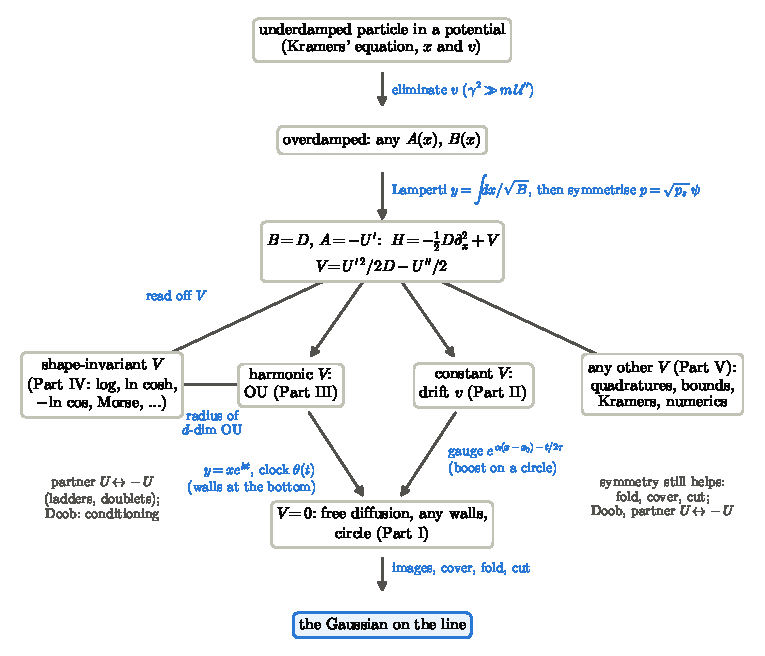
\includegraphics[width=\linewidth]{reductions.pdf}
  \caption{How the problems reduce. Each arrow points to a simpler problem and is labelled by the move that gets
  there. Everything that is solvable in closed form ends at the Gaussian.}
  \label{fig:reductions}
\end{figure}

\subsection{A procedure for a new problem}

\begin{enumerate}
  \item \textbf{Physics to equation.} For a particle with inertia, check that it is overdamped, $m|\mathcal U''|\ll\gamma^2$
        (\cref{sec:physical}). Otherwise the problem lives in $(x,v)$ and the rest of these notes does not apply
        directly.
  \item \textbf{Classify the boundaries} (\cref{tab:feller}). Only a regular boundary needs, or allows, a condition;
        at an interface, decide which density is continuous (\cref{sec:interface}).
  \item \textbf{Make $B$ constant} with the Lamperti change of variable (\cref{sec:general}).
  \item \textbf{Use the symmetries of the domain.} A mirror symmetry means images, or folding into sectors; a
        periodic domain means the cover; a target point means cutting there.
  \item \textbf{Symmetrise and read off $V=U'^2/2D-U''/2$} (\cref{sec:operator}).
        \begin{itemize}
          \item $V$ constant: the free problem (Part~I), with every rate raised by $V$ and Robin walls. Without walls,
                a boost does the same with no cost.
          \item $V$ harmonic: OU. With walls only at the bottom, map to the free problem; otherwise use Kummer
                functions.
          \item $V$ shape-invariant (\cref{tab:solvable}): the spectrum follows by algebra.
          \item Anything else: exact quadratures for $p_s$ and every first-passage quantity, bounds on the gap,
                small-noise ladders and Kramers rates, and numerics (\cref{sec:general}).
        \end{itemize}
  \item \textbf{Transform the question as well as the problem.} Conditioned paths call for a Doob transform. A
        question about $-U$ calls for the partner. First-passage questions go to the backward equation. Winding
        on a circle goes to the tilted generator.
  \item \textbf{Track the walls and the rates} through every step, using \cref{tab:reductions}. A wall that moves
        under a map, or turns into a Robin condition, is where a closed form usually stops.
\end{enumerate}

\subsection{Chains back to the Gaussian}

Each line follows one problem down to something already solved:
\begin{itemize}
  \item drift toward an absorbing wall (\cref{sec:drift-hl-absorbing}) $\xrightarrow{\text{gauge}}$ free absorbing
        half-line (\cref{sec:hl-absorbing}) $\xrightarrow{\text{one image}}$ Gaussian;
  \item OU absorbed at the bottom (\cref{sec:ou-hl-absorbing}) $\xrightarrow{\text{map}}$ free absorbing half-line
        $\xrightarrow{\text{image}}$ Gaussian;
  \item radial OU in three dimensions (\cref{sec:radial}) $\xrightarrow{\text{Doob},\ h=x}$ OU absorbed at the
        bottom $\xrightarrow{\text{map, image}}$ Gaussian; or directly, as the projection of the 3D Gaussian;
  \item square-root process absorbed at the origin (\cref{sec:sqrt}) $\xrightarrow{y=r^2}$ radial motion in dimension
        $d$ $\xrightarrow{\text{Doob}}$ radial motion in dimension $4-d$ $\xrightarrow{\text{projection}}$ Gaussian (for
        integer $d$; otherwise the chain ends at the Bessel function);
  \item step in $D$ (\cref{sec:interface}) $\xrightarrow{\text{partial image}}$ Gaussian;
  \item constant drift on a circle (\cref{sec:drift-circle}) $\xrightarrow{\text{boost}}$ free circle
        (\cref{sec:circle}) $\xrightarrow{\text{cover}}$ Gaussian;
  \item free circle $\xrightarrow{\text{fold}}$ reflecting interval of half the length (\cref{sec:reflecting})
        $\xrightarrow{\text{images}}$ Gaussian;
  \item mixed interval (\cref{sec:mixed}) $\xrightarrow{\text{unfold}}$ absorbing interval of length $2L$
        (\cref{sec:absorbing}) $\xrightarrow{\text{images}}$ Gaussian;
  \item OU on a circle (\cref{sec:ou-circle}) $\xrightarrow{\text{fold}}$ OU reflecting and absorbing intervals
        (\cref{sec:ou-reflecting,sec:ou-absorbing}), related by the partner ladder. The chain stops here at Kummer
        roots, because the far wall moves under the map;
  \item mixed interval with drift (\cref{sec:drift-mixed}) $\xrightarrow{\text{gauge}}$ free problem with a Robin and
        a Dirichlet wall. The chain stops at the root condition $\tan kL=-k/\alpha$;
  \item double well (\cref{sec:double-well}) $\xrightarrow{\text{symmetrise}}$ a Schr\"odinger operator with no
        closed form. The chain ends in numerics, or in small-noise asymptotics: local OU ladders and Kramers rates.
\end{itemize}

% ==============================================================================
\appendix
\crefalias{section}{appendix}
\section{Figures and numerical checks}
\label{app:checks}

The script \texttt{scripts/make\_figures.py} needs numpy, scipy and matplotlib (the conda env
\texttt{research} has all three). Run from the \texttt{fpe-examples} folder,
\begin{center}
  \texttt{python scripts/make\_figures.py} \quad or \quad \texttt{python scripts/make\_figures.py mixed line}
\end{center}
to redo every section or just the named ones (the keys of \texttt{SECTIONS} in the script). It writes the
figures to \texttt{figures/} and prints a list of checks. All of the following pass.
\begin{itemize}
  \item Image sum $=$ mode sum for $p$ on every interval, at $Dt/L^2=0.02$ and $0.2$ (to $10^{-15}$).
  \item Normalisation, $\avg x$ and $\avg{x^2}$ series vs.\ quadrature of $p$; $C(0)=L^2/12$; folded-normal
        $\avg x$ and $\avg{x^2}=x_0^2+Dt$ on the half-line.
  \item $S$ series vs.\ quadrature of $p$; image forms of the exit fluxes vs.\ $-\partial_tS$ series;
        $S=\operatorname{erf}(x_0/\sqrt{2Dt})$ vs.\ quadrature.
  \item $\int f\,\dd t=1$ (or $1-S$ on the half-line), $\int j_L\,\dd t=\pi_L$, and $T$,
        $\operatorname{Var}T$, $T_0$, $T_L$ from quadrature of the fluxes vs.\ the closed forms; mode and median
        of the L\'evy--Smirnov density.
  \item $\int q_\infty T\,\dd x_0=1/\lambda_{\min}$ for every QSD on an interval; the Rayleigh limit at
        $Dt/x_0^2=10^4$; the resolvent \cref{eq:L-resolvent}.
  \item Drift (Part II), for several $v$ of both signs: the PDE residual of each propagator by finite
        differences (below $10^{-4}$ relative); $J=0$ at reflecting walls and $p=0$ at absorbing ones;
        normalisation; $\avg{x(t)}\approx x_0+vt$ at $Dt/L^2=10^{-3}$, which checks the initial condition;
        mode sums vs.\ quadrature; $\pi_L$, $T$, $T_0$, $T_L$ from quadrature of the exit fluxes; $T_L$ even in
        $v$; inverse-Gaussian moments and escape probability; $S$ against its $t^{-3/2}e^{-v^2t/2D}$ asymptote;
        and the eigen-equation residual of the half-line QSDs.
  \item Ornstein--Uhlenbeck (Part III):
        \begin{itemize}
          \item the map \cref{eq:ou-map} against the line and half-line propagators (to $10^{-15}$);
          \item the Mehler sum against the Gaussian;
          \item PDE residuals, wall conditions and normalisation for every geometry;
          \item survival, $T$ and $\pi_L$ from the closed forms against quadrature, against
                $\sum_nc_n/\lambda_n$, and against the integrated exit flux;
          \item $\int q_\infty T=1/\lambda_{\min}$;
          \item the reflecting-equals-absorbing-plus-$k$ ladder (to $10^{-15}$);
          \item the $L\to0$ and $L\to\infty$ limits of every slowest rate;
          \item $\lambda_0T(0)\to1$ for Kramers;
          \item the constant $\ln2+\gamma_{\rm E}/2$;
          \item the heavy-tailed QSDs $q_\nu$: normalisation, eigen-equation residual, tail exponent $-1-\nu$,
                and exact evolution as $e^{-\nu kt}q_\nu$ through the map.
        \end{itemize}
        The interval eigenvalues come from root-finding on the Kummer functions \cref{eq:kummer} with
        \texttt{scipy.special.hyp1f1}. They were checked against \texttt{mpmath} to machine precision.
  \item The physical model (\cref{sec:physical}): the closed-form position correlation of the damped oscillator
        against the regression equation, integrated numerically, for $\zeta=0.25$, $1$, $3$ (to $10^{-11}$); the
        slowest rate at critical damping ($2\mathcal K/\gamma$) and at $\zeta=10$ against the corrected Smoluchowski
        value $1+1/4\zeta^2$; and the Maxwell--Boltzmann density as a stationary solution of Kramers' equation in a
        double well.
  \item The symmetrised operator \cref{eq:schrodinger}, solved by finite differences (4000 points, Robin
        walls by ghost points), against the spectra found from the forward equation: the drift interval with
        reflecting walls; OU intervals with reflecting and absorbing walls (Kummer roots); the cosine circle at
        $\kappa=3$ and $16$ (Fourier recurrence); and the sawtooth circle with the $\delta$-spike at the cusp. All
        agree to about $10^{-5}$, relative.
  \item Part IV: the spectra of all six shape-invariant potentials of \cref{tab:solvable} from finite differences
        of $H$ (the two not worked out included, to $10^{-3}$ or better); the partner identities
        $\tilde V(s)=V(s')+R(s)$ (to $10^{-12}$); the radial propagators against the angular integral of the 2D
        Gaussian, the $d=1$ images, the $d=3$ Doob form and the Laguerre series (to $10^{-12}$), their PDE
        residual, and the recurrence probability; the Jacobi and Gegenbauer eigenfunctions (residuals), the
        normalisations, the Gegenbauer propagator, $\avg{\sin(x/w)}$, the Bakry--\'Emery and variance bounds, the
        Wright--Fisher transformation, and the $s=\frac12$ case as rotational diffusion on the sphere (drift,
        Legendre eigenfunctions, Debye rate).
  \item Part V, the double well, with the detailed-balance jump discretisation: convergence of $\lambda_1$;
        $\lambda_1$ against \G{9.2.18} (to $2\times10^{-5}$ at $\beta=12$) and Kramers (to $2.5\,\%$ at $\beta=16$);
        $\lambda_1T/2=1$ with $T$ from \G{5.2.160}; $\lambda_2\to|U''(0)|$ and $\lambda_3\to U''(a)$ at $\beta=80$;
        $Q_1=2\pi_c-1$; and the two-state population law.
  \item Part VI:
        \begin{itemize}
          \item the interface: normalisation, the jump by $K$, continuity of the flux and the free equation on each side,
                for four values of $K$; the smoothed step, solved by finite differences (Crank--Nicolson), against the
                partial image for all three readings, with an error proportional to $\varepsilon$ (about $1\,\%$ at
                $\varepsilon=0.01a$); $\pi_+$ and $T$ against Gardiner's quadratures; $T(0)$ against the three means; the
                box rates against a jump process with exact detailed balance; and simulations of the smoothed SDE;
          \item the square-root process: normalisation of $p_+$; $\int p_-=P(1-\frac d2,z_t)$ for five values of $d$, and
                the extinction probability; PDE residuals; $p_+$ against the radial propagator, and the Doob relation
                (both to $10^{-15}$); $J(0)=0$ when reflected and $J(0)=\dot S$ when absorbed; the power laws at the
                origin; $T$ against \G{5.2.161}; both Laguerre ladders and the decay rate of $S$; the QSDs (residual,
                normalisation, positivity, tails) and the Yaglom limit; the exact sampler behind the figure;
          \item the QIF neuron: $1/J_s$ against \G{5.2.160} on a grid; its three limits; normalisation and tails of $p_s$;
                the density at $\theta=\pi$; the Itô form of the $\theta$ equation; simulations of $\theta$ at eleven
                parameter values; and, for the drifting circle through $\tan(\theta/2)$, the Cauchy density's constant
                current and the integrability of $f$ and $g$;
          \item Feller's test \G{5.2.25}--\G{5.2.29}, with shrinking cutoffs, for the square-root process in $y$ and in
                $r$, Gardiner's reaction model and geometric Brownian motion; the map from $x$ to $\ln x$ onto the Morse
                drift; and the rates of neutral Wright--Fisher from finite differences.
        \end{itemize}
  \item Gardiner's $P_\lambda$ and $Q_\lambda$ as named in the boxes (section \texttt{pq} of the script):
        \begin{itemize}
          \item biorthonormality $\int P_nQ_m=\delta_{nm}$ \G{5.2.79}, with $P=p_sQ$, for the free and drift intervals,
                the circle (with and without drift), Hermite on the line and half-lines, the Kummer intervals, the
                sawtooth circle (both sectors together), the Laguerre ladder of \cref{sec:radial}, the bound states of
                $\ln\cosh$, the normalised Gegenbauer $Q_n$, the interface box ($\chi=1$, $0$) and both Laguerre
                ladders of the square-root process (also at an exit, $d=-0.5$);
          \item forward and backward eigen-equation residuals on the intervals and circles, and on the drift mixed
                interval the wall conditions $J(P)=Q'=0$ at $0$ and $P=Q=0$ at $L$;
          \item $\sum P_n(x)Q_n(x_0)e^{-\lambda_nt}$, or its integral over a continuous label, against the propagators
                of the line (free and drifting, gauge and Fourier modes), the half-lines (free; drift, with the
                Robin continuum and the bound state $P_0=p_s$), OU on the half-lines, the sawtooth circle, the Bessel
                process and $p_\pm$ of the square-root process, to $10^{-6}$ or better;
          \item on the cosine circle, left and right eigenvectors of \cref{eq:cos-recurrence} as $Q_\lambda$ and
                $P_\lambda$; $P_\lambda/p_s$ is a backward eigenfunction without tilt and is not with tilt;
          \item the double well: $\int p_s(2\pi_c-1)^2=1$ to $10^{-3}$, the normalised $Q_1$ against $2\pi_c-1$, and
                the hilltop mode at $\beta=80$.
        \end{itemize}
  \item Which QSD is reached (\cref{sec:spectrum-states}): for drift toward the wall, an exponential start
        $e^{-x/2\ell}$ converges to the QSD with the same tail and decays at $\beta|v|-\frac12D\beta^2$, while
        $e^{-2x/\ell}$ converges to the edge QSD with an error $\propto1/t$. For OU, a start with tail
        $x^{-3/2}$ converges to $q_{1/2}$ with $S\propto e^{-kt/2}$, while a tail $x^{-5/2}$ (finite mean)
        converges to the Rayleigh QSD.
  \item Circles, in all three parts:
        \begin{itemize}
          \item image sum against mode sum, normalisation and PDE residuals; the fold onto the reflecting
                interval of half the length (to $10^{-15}$);
          \item $\avg{e^{iq_1x}}$ against the complex eigenvalue; $J_s=v/L$; the twisted periodicity of the
                gauged $u$; \G{5.2.46} as printed equals $-2$ times the corrected form;
          \item the cut-invariant $p_s$ \cref{eq:circle-ps} against \G{5.2.47} with the seam at $0$ and against
                the Fourier null vector, with and without tilt;
          \item $v_{\rm w}$ and $D_{\rm eff}$ three ways: $LJ_s$; $\Lambda'(0)$ and $\Lambda''(0)$ from
                \cref{eq:cos-recurrence}; and an independent jump-process discretisation of the generator on a
                ring of 4000 sites;
          \item Lifson--Jackson against $L^2/T_{\rm w}$ from \G{5.2.158} on the cover; $T_{\rm w}$ independent
                of the start; the Einstein relation; the Kramers limit;
          \item for the sawtooth: continuity of $J$ at the cusp, the splitting by exactly $k$, and
                $D_{\rm eff}=\tfrac12L^2\lambda_0^{\rm mix}$ at $L=8\ell$;
          \item for the cosine well: the exact doublets, the $\kappa\to0$ and $\kappa\to\infty$ limits, and a
                simulation of the tilted lift ($v_{\rm w}$ and $D_{\rm eff}$ within statistical error).
        \end{itemize}
\end{itemize}
Simulation: Euler steps of $\dd x=\sqrt D\,\dd W$ with $\Delta t=10^{-4}$ or $2\times10^{-4}\,L^2/D$, plus a
Brownian-bridge test for crossings within a step (crossing probability $e^{-2x_ax_b/D\Delta t}$ for the wall
at $0$). A reflecting wall at $0$ folds the path, $x\to\lvert x\rvert$, which is exact. With 4000 paths per
starting point, $T$ and $\pi_L$ agree with the closed forms to within about two standard errors.

To add a figure, write a \texttt{fig\_*} function in the script, register it in \texttt{SECTIONS} with its
checks, and \verb|\includegraphics| the PDF. Screenshots from \texttt{sde-explorer} can go in
\texttt{figures/} too.

\begin{thebibliography}{99}
\bibitem{gardiner} C.~W. Gardiner, \emph{Handbook of Stochastic Methods for Physics, Chemistry and the
  Natural Sciences}, 2nd ed.\ (Springer, 1985). \S5.2.
\bibitem{redner} S.~Redner, \emph{A Guide to First-Passage Processes} (Cambridge University Press, 2001).
\bibitem{collet} P.~Collet, S.~Mart\'inez and J.~San~Mart\'in, \emph{Quasi-Stationary Distributions}
  (Springer, 2013).
\bibitem{lifson} S.~Lifson and J.~L. Jackson, On the self-diffusion of ions in a polyelectrolyte solution,
  J.~Chem.\ Phys.\ \textbf{36}, 2410 (1962).
\bibitem{risken} H.~Risken, \emph{The Fokker--Planck Equation}, 2nd ed.\ (Springer, 1989).
\bibitem{perrin} J.~Perrin, Mouvement brownien et r\'ealit\'e mol\'eculaire, Ann.\ Chim.\ Phys.\ (8)
  \textbf{18}, 5 (1909).
\bibitem{gerstein} G.~L. Gerstein and B.~Mandelbrot, Random walk models for the spike activity of a single
  neuron, Biophys.\ J.\ \textbf{4}, 41 (1964).
\bibitem{ambegaokar} V.~Ambegaokar and B.~I. Halperin, Voltage due to thermal noise in the dc Josephson effect,
  Phys.\ Rev.\ Lett.\ \textbf{22}, 1364 (1969).
\bibitem{leegrier} S.-H. Lee and D.~G. Grier, Giant colloidal diffusivity on corrugated optical vortices,
  Phys.\ Rev.\ Lett.\ \textbf{96}, 190601 (2006).
\bibitem{blickle} V.~Blickle, T.~Speck, C.~Lutz, U.~Seifert and C.~Bechinger, Einstein relation generalized to
  nonequilibrium, Phys.\ Rev.\ Lett.\ \textbf{98}, 210601 (2007).
\bibitem{mccann} L.~I. McCann, M.~Dykman and B.~Golding, Thermally activated transitions in a bistable
  three-dimensional optical trap, Nature \textbf{402}, 785 (1999).
\bibitem{prieve} D.~C. Prieve, F.~Luo and F.~Lanni, Brownian motion of a hydrosol particle in a colloidal force
  field, Faraday Discuss.\ Chem.\ Soc.\ \textbf{83}, 297 (1987).
\bibitem{hanggi} P.~H\"anggi, P.~Talkner and M.~Borkovec, Reaction-rate theory: fifty years after Kramers,
  Rev.\ Mod.\ Phys.\ \textbf{62}, 251 (1990).
\bibitem{cooper} F.~Cooper, A.~Khare and U.~Sukhatme, Supersymmetry and quantum mechanics, Phys.\ Rep.\
  \textbf{251}, 267 (1995).
\bibitem{bakry} D.~Bakry, I.~Gentil and M.~Ledoux, \emph{Analysis and Geometry of Markov Diffusion Operators}
  (Springer, 2014).
\bibitem{cattiaux} P.~Cattiaux, P.~Collet, A.~Lambert, S.~Mart\'inez, S.~M\'el\'eard and J.~San~Mart\'in,
  Quasi-stationary distributions and diffusion models in population dynamics, Ann.\ Probab.\ \textbf{37},
  1926 (2009).
\bibitem{martinez} S.~Mart\'inez, P.~Picco and J.~San~Mart\'in, Domain of attraction of quasi-stationary
  distributions for the Brownian motion with drift, Adv.\ Appl.\ Probab.\ \textbf{30}, 385 (1998).
\bibitem{lladser} M.~Lladser and J.~San~Mart\'in, Domain of attraction of the quasi-stationary distributions
  for the Ornstein--Uhlenbeck process, J.~Appl.\ Probab.\ \textbf{37}, 511 (2000).
\bibitem{reimann} P.~Reimann, C.~Van~den~Broeck, H.~Linke, P.~H\"anggi, J.~M. Rubi and A.~P\'erez-Madrid,
  Giant acceleration of free diffusion by use of tilted periodic potentials, Phys.\ Rev.\ Lett.\ \textbf{87},
  010602 (2001).
\bibitem{volpe} G.~Volpe, L.~Helden, T.~Brettschneider, J.~Wehr and C.~Bechinger, Influence of noise on force
  measurements, Phys.\ Rev.\ Lett.\ \textbf{104}, 170602 (2010).
\bibitem{tailleur} J.~Tailleur and M.~E. Cates, Statistical mechanics of interacting run-and-tumble bacteria,
  Phys.\ Rev.\ Lett.\ \textbf{100}, 218103 (2008).
\bibitem{crank} J.~Crank, \emph{The Mathematics of Diffusion}, 2nd ed.\ (Oxford University Press, 1975), ch.~12.
\bibitem{sancho} J.~M. Sancho, M.~San~Miguel and D.~D\"urr, Adiabatic elimination for systems of Brownian particles
  with nonconstant damping coefficients, J.~Stat.\ Phys.\ \textbf{28}, 291 (1982).
\bibitem{lejay} A.~Lejay, On the constructions of the skew Brownian motion, Probab.\ Surveys \textbf{3}, 413 (2006).
\bibitem{feller51} W.~Feller, Two singular diffusion problems, Ann.\ Math.\ \textbf{54}, 173 (1951).
\bibitem{cir} J.~C. Cox, J.~E. Ingersoll and S.~A. Ross, A theory of the term structure of interest rates,
  Econometrica \textbf{53}, 385 (1985).
\bibitem{manning} G.~S. Manning, Limiting laws and counterion condensation in polyelectrolyte solutions I.
  Colligative properties, J.~Chem.\ Phys.\ \textbf{51}, 924 (1969).
\bibitem{ermentrout} G.~B. Ermentrout and N.~Kopell, Parabolic bursting in an excitable system coupled with a slow
  oscillation, SIAM J.~Appl.\ Math.\ \textbf{46}, 233 (1986).
\bibitem{lindner} B.~Lindner, A.~Longtin and A.~Bulsara, Analytic expressions for rate and CV of a type I neuron
  driven by white Gaussian noise, Neural Comput.\ \textbf{15}, 1761 (2003).
\end{thebibliography}

\end{document}

% ==============================================================================
% TEMPLATE FOR A NEW EXAMPLE: copy above \appendix, and add a row to tab:overview and tab:physical.
%
% \section{<short name>}
% \label{sec:<key>}
%
% \begin{keyresults}
% $A=\dots$, $B=\dots$ on $(\dots)$, walls: \dots. SDE $\dd x=\dots$. Gardiner \Gs{\dots}.
% \begin{align}
%   \lambda_n &= \dots \qquad P_n(x)=\dots,\quad Q_n(x)=\dots \\
%   p(x,t\given x_0,0) &= \dots \\
%   \text{long-time state / slowest rate} &= \dots \\
%   \text{first passage}: \pi_a,\ T(x_0),\ \dots
% \end{align}
% \end{keyresults}
%
% \paragraph{Physical picture.} An overdamped particle in $\mathcal U=\dots$; what the walls are.
%
% \paragraph{From Gardiner.} Which equations of the book give the boxed results.
%
% \subsection{Spectrum and propagator}
% \subsection{Long-time behaviour}
% \subsection{Moments and correlations}
% \subsection{First passage}
% \subsection{Open questions}
%
% \begin{figure}[tbp]
%   \centering
%   \includegraphics[width=\linewidth]{<file>.pdf}
%   \caption{\dots}
%   \label{fig:<key>}
% \end{figure}
